\section{Results}

\subsection{Dataset Characterization}

The dataset scraped from Crunchbase contains data about 22,527 companies (startups, ...), 38,843 investors, and 147,832 invesments.

After the data cleaning process described in the \textit{Methodology} section, the dataset used to further generate the syndication networks yields 104,618 investment records, representing transactions among 16,932 companies and 11,279 investors, totaling \$3.19 tri USD invested from 1990 until 2025, even though we are going to concentrate on invesment data among the 20 years window from 2004 to 2024.

\subsubsection{Syndication Trends}

A significant part of these investments records represent syndicated investments, as showed in figure \ref{fig:syndication_evolution}.

\begin{figure}[htbp]
\centering
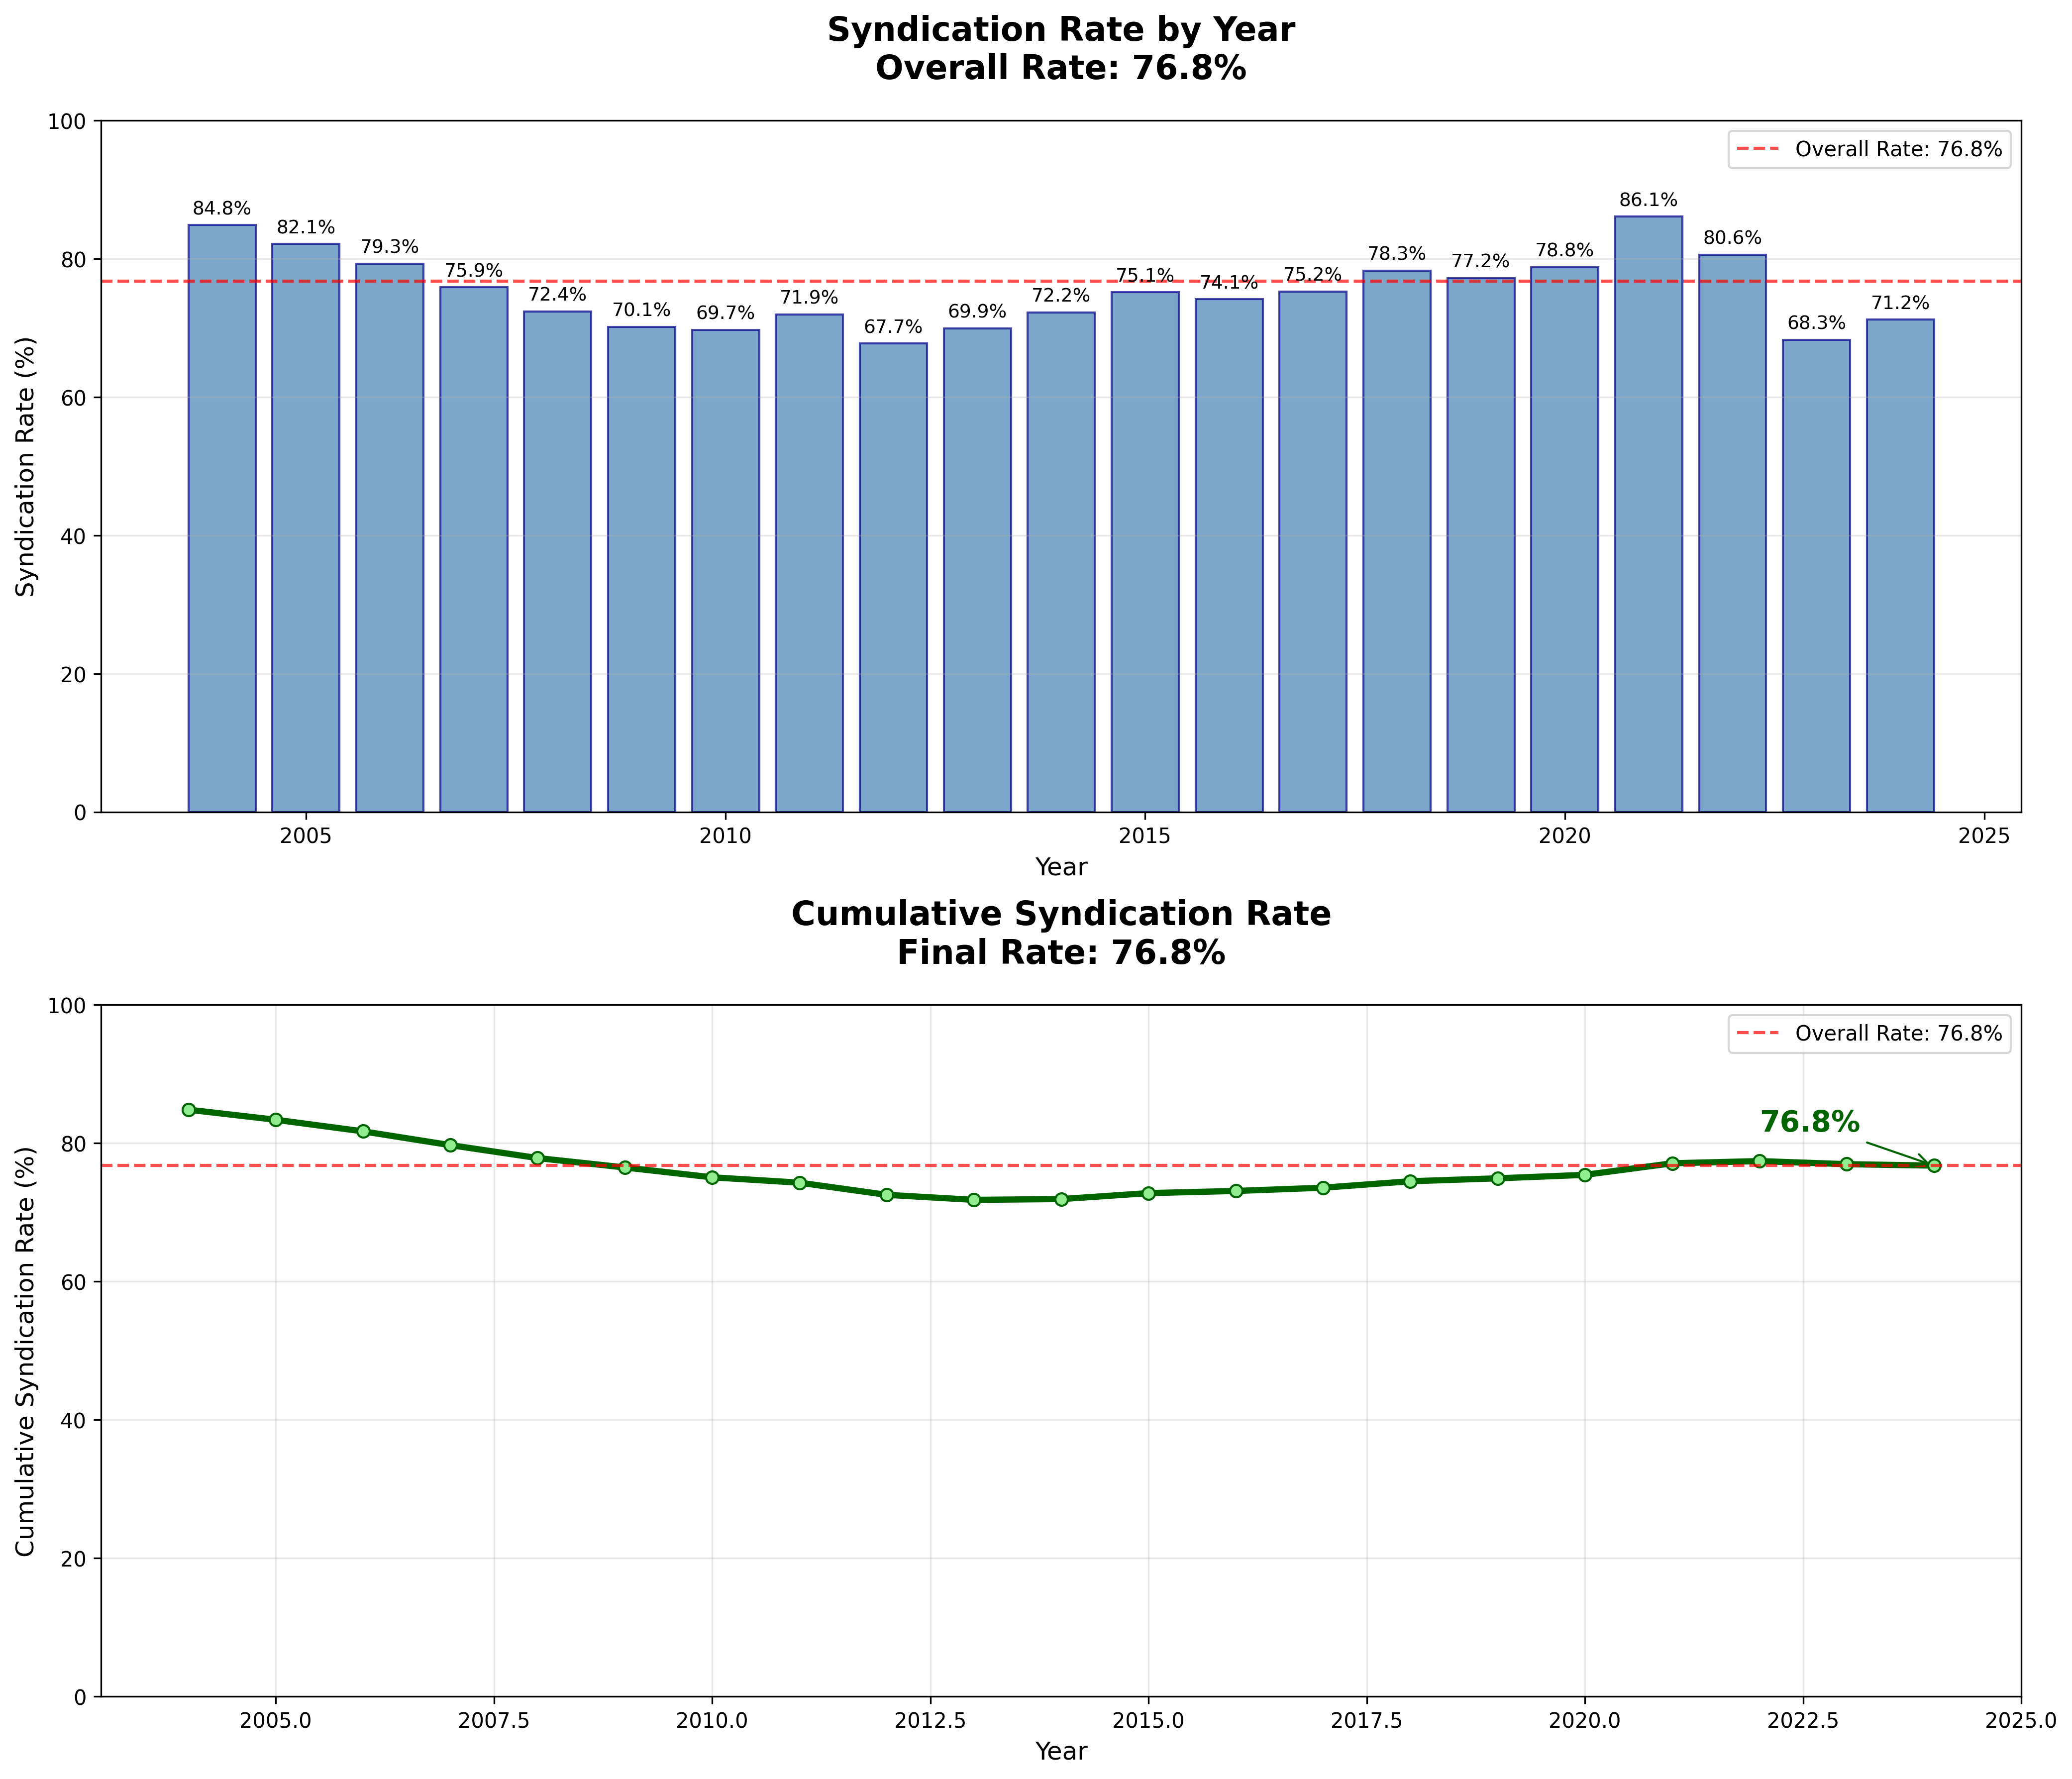
\includegraphics[width=1\textwidth]{../figures/us/syndication_trends.png}
\caption{Evolution of syndicated investment trends in the Crunchbase dataset. The figure illustrates changes in the proportion and of syndicated investments over time, highlighting the prevalence of co-investment activity among venture capital investors.}
\label{fig:syndication_evolution}
\end{figure}

\subsubsection{Investment Activity}

Figure \ref{fig:vc_investment_activity} presents the overall investment activity trends, while Figure \ref{fig:investment_temporal_evolution} provides a detailed breakdown of temporal patterns across different investment characteristics.

\begin{figure}[htbp]
\centering
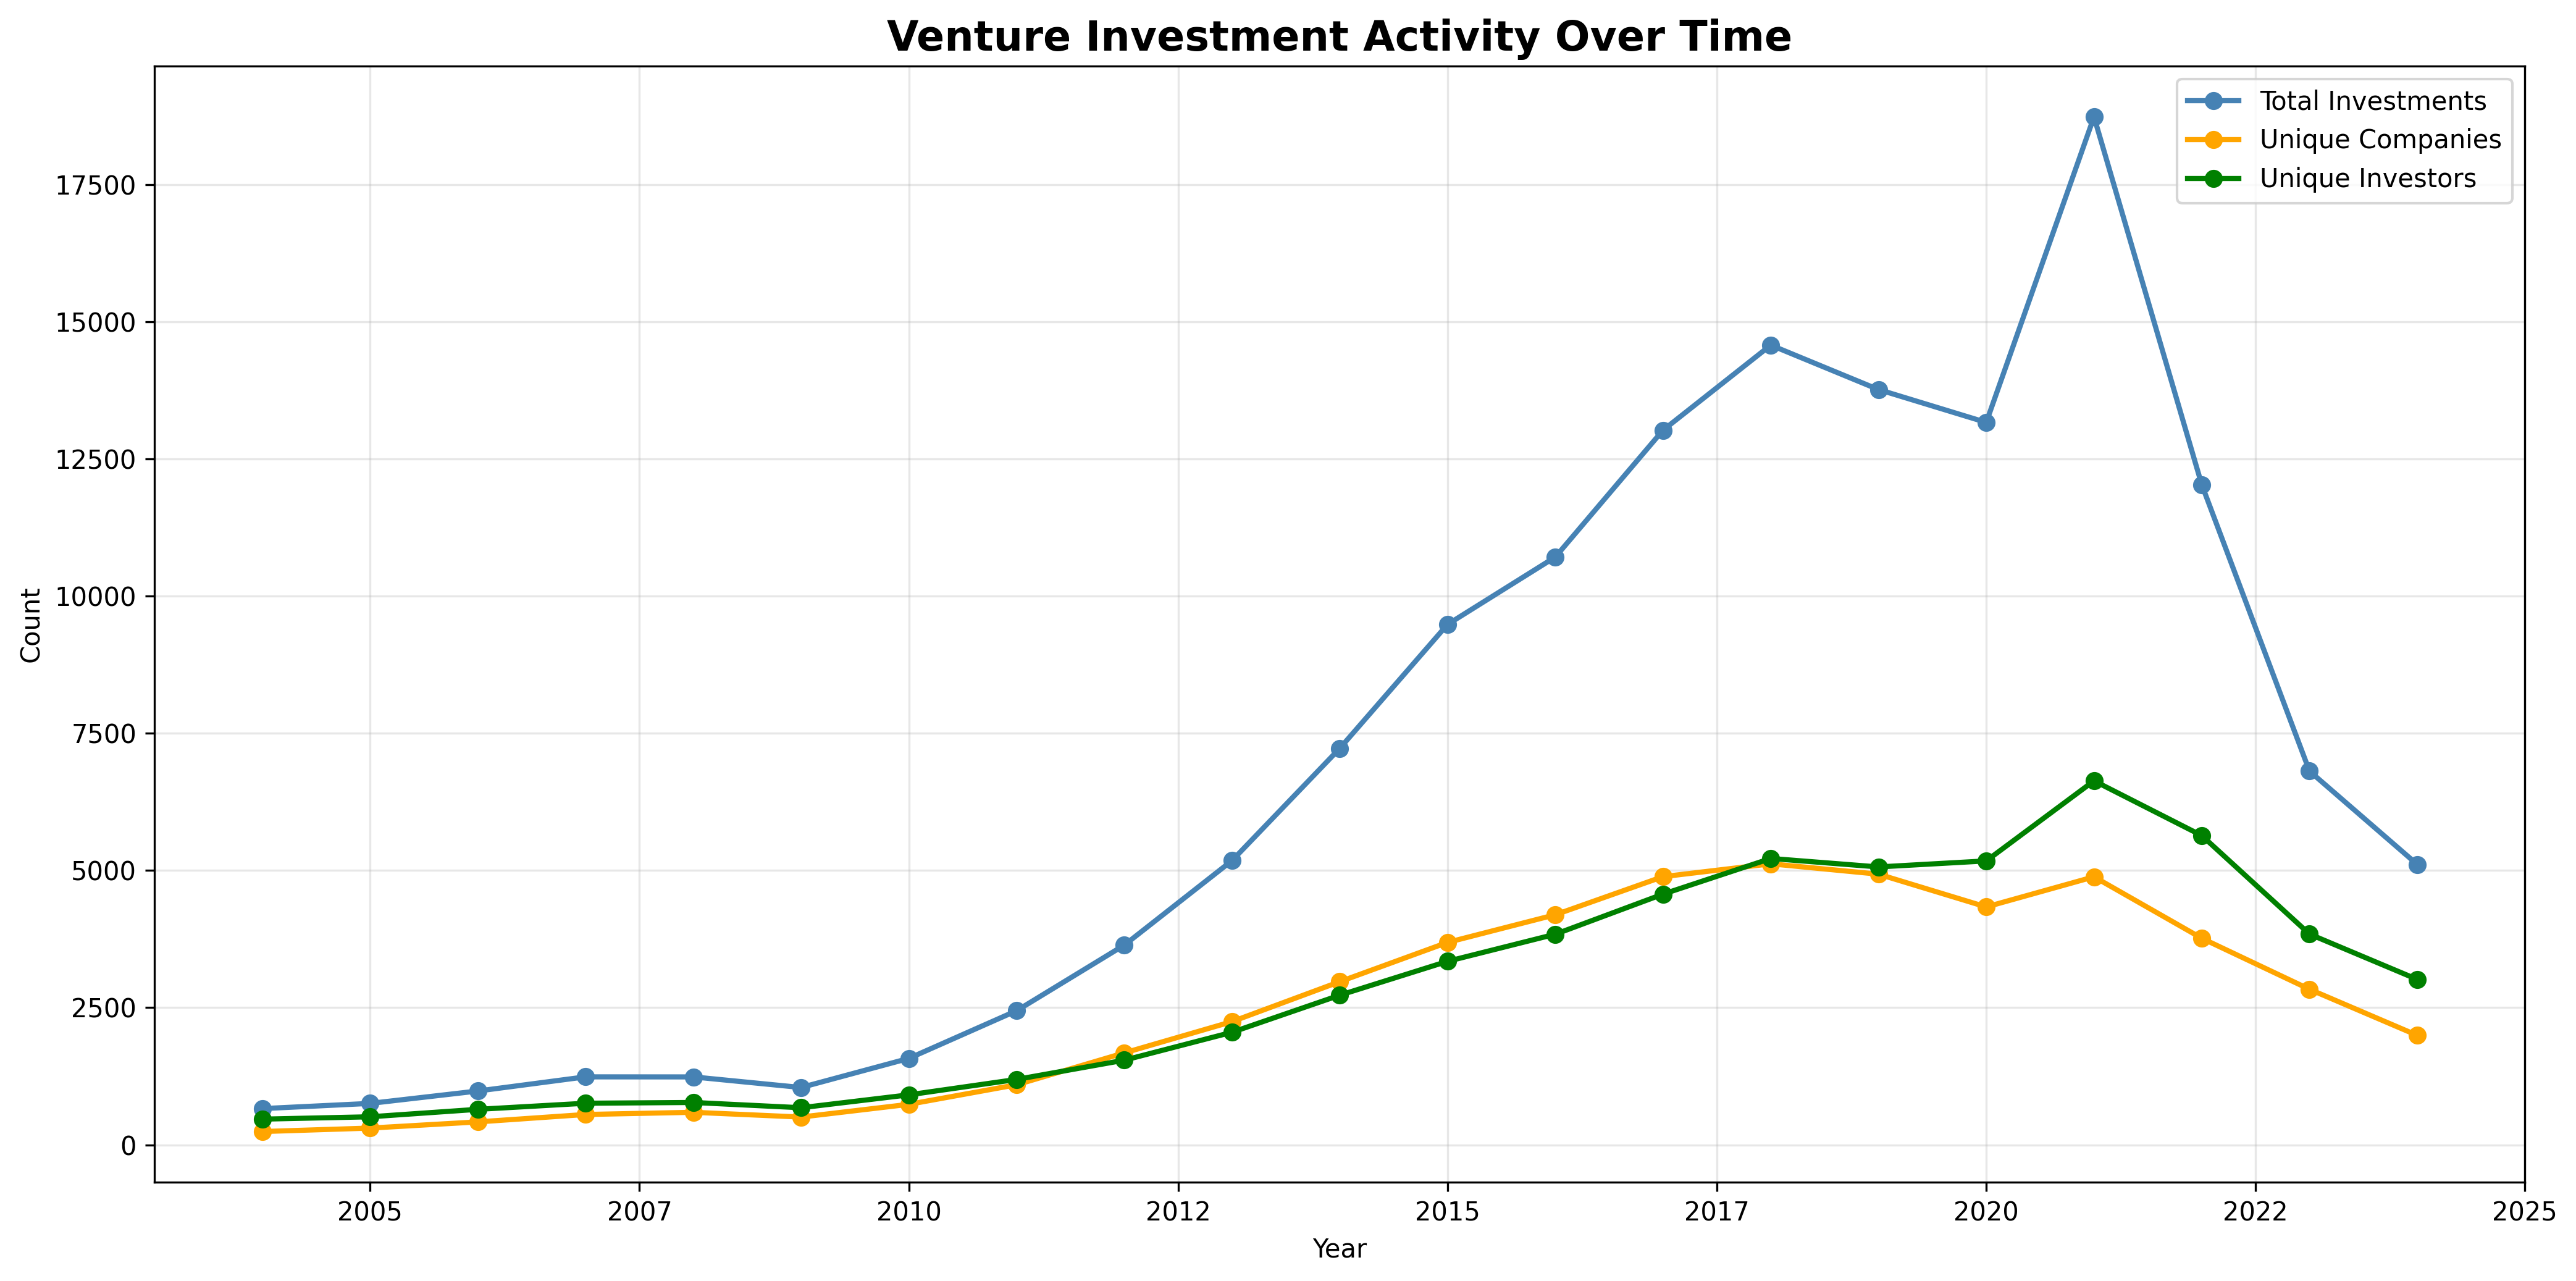
\includegraphics[width=1\textwidth]{../figures/us/vc_investment_activity_over_time.png}
\caption{Venture capital investment activity over time. The figure shows the evolution of investment transactions and funding patterns across the study period, highlighting major trends and cyclical patterns in venture capital deployment.}
\label{fig:vc_investment_activity}
\end{figure}

\begin{figure}[htbp]
\centering
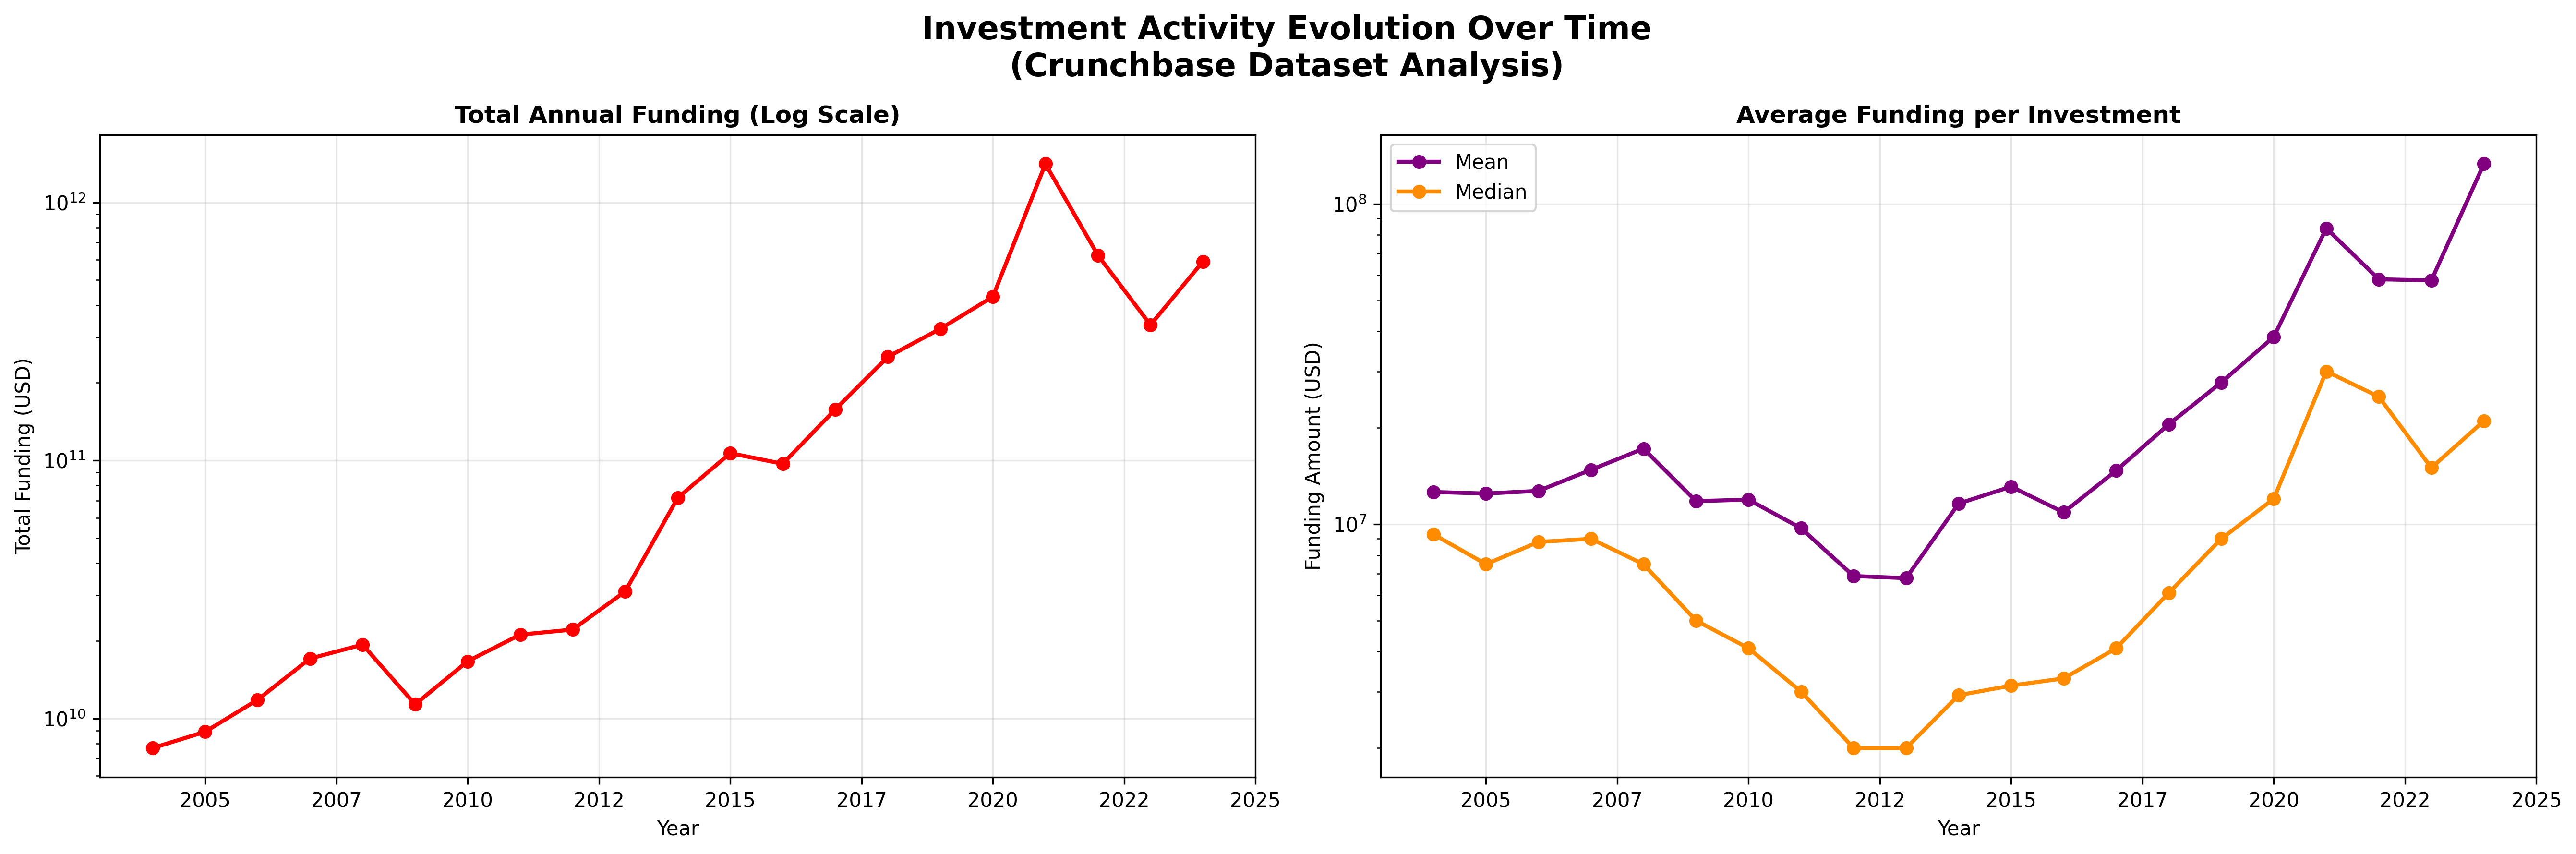
\includegraphics[width=1\textwidth]{../figures/us/investment_funding_temporal_evolution.png}
\caption{Temporal evolution of investment activity characteristics. This comprehensive view illustrates how different aspects of venture capital investment behavior have changed over time, including variations in funding amounts, transaction frequency, and market participation patterns.}
\label{fig:investment_temporal_evolution}
\end{figure}

The investment activity data demonstrates clear temporal variations that might reflect broader economic cycles and venture capital market maturation. 

The analysis reveals growth in venture capital activity over the study period, with remarkable acceleration followed by decreasing period in recent years. From 2004 to 2024, the venture capital ecosystem experienced substantial expansion, with total investments increasing by 674.5\% and unique investors growing by 544.4\%.

The year 2021 emerged as a unique moment for venture capital activity, representing peak performance across multiple dimensions. This year recorded the highest number of investments (18,741 transactions), the largest total funding amount (\$1.41 trillion), and the greatest investor participation (6,636 unique investors). This convergence of peak metrics in 2021 reflects both the maturation of the venture capital industry and the exceptional market conditions during the post-pandemic economic recovery.

The analysis reveals that investment frequency and average funding amounts do not necessarily follow identical temporal patterns. While transaction volumes may increase during certain periods, average investment sizes can exhibit different trends, suggesting varying risk appetites and market conditions across different time windows. 

The substantial growth rates observed between 2004 and 2024 indicate not only market expansion but also the increasing institutionalization of venture capital as an asset class.

These temporal patterns provide important context for understanding the network structures observed in the community analysis, as investment behaviors and syndication patterns may be influenced by the broader economic environment during different time periods. 

\todo[inline]{add insights from Crunchbase posts on why investment activities are decreasing}

\subsubsection{Investment Stages Evolution}

Figures \ref{fig:investment_stage_dist} and \ref{fig:investment_stage_temporal} illustrates the analysis of investment stages over time across the venture capital ecosystem

\begin{figure}[htbp]
\centering
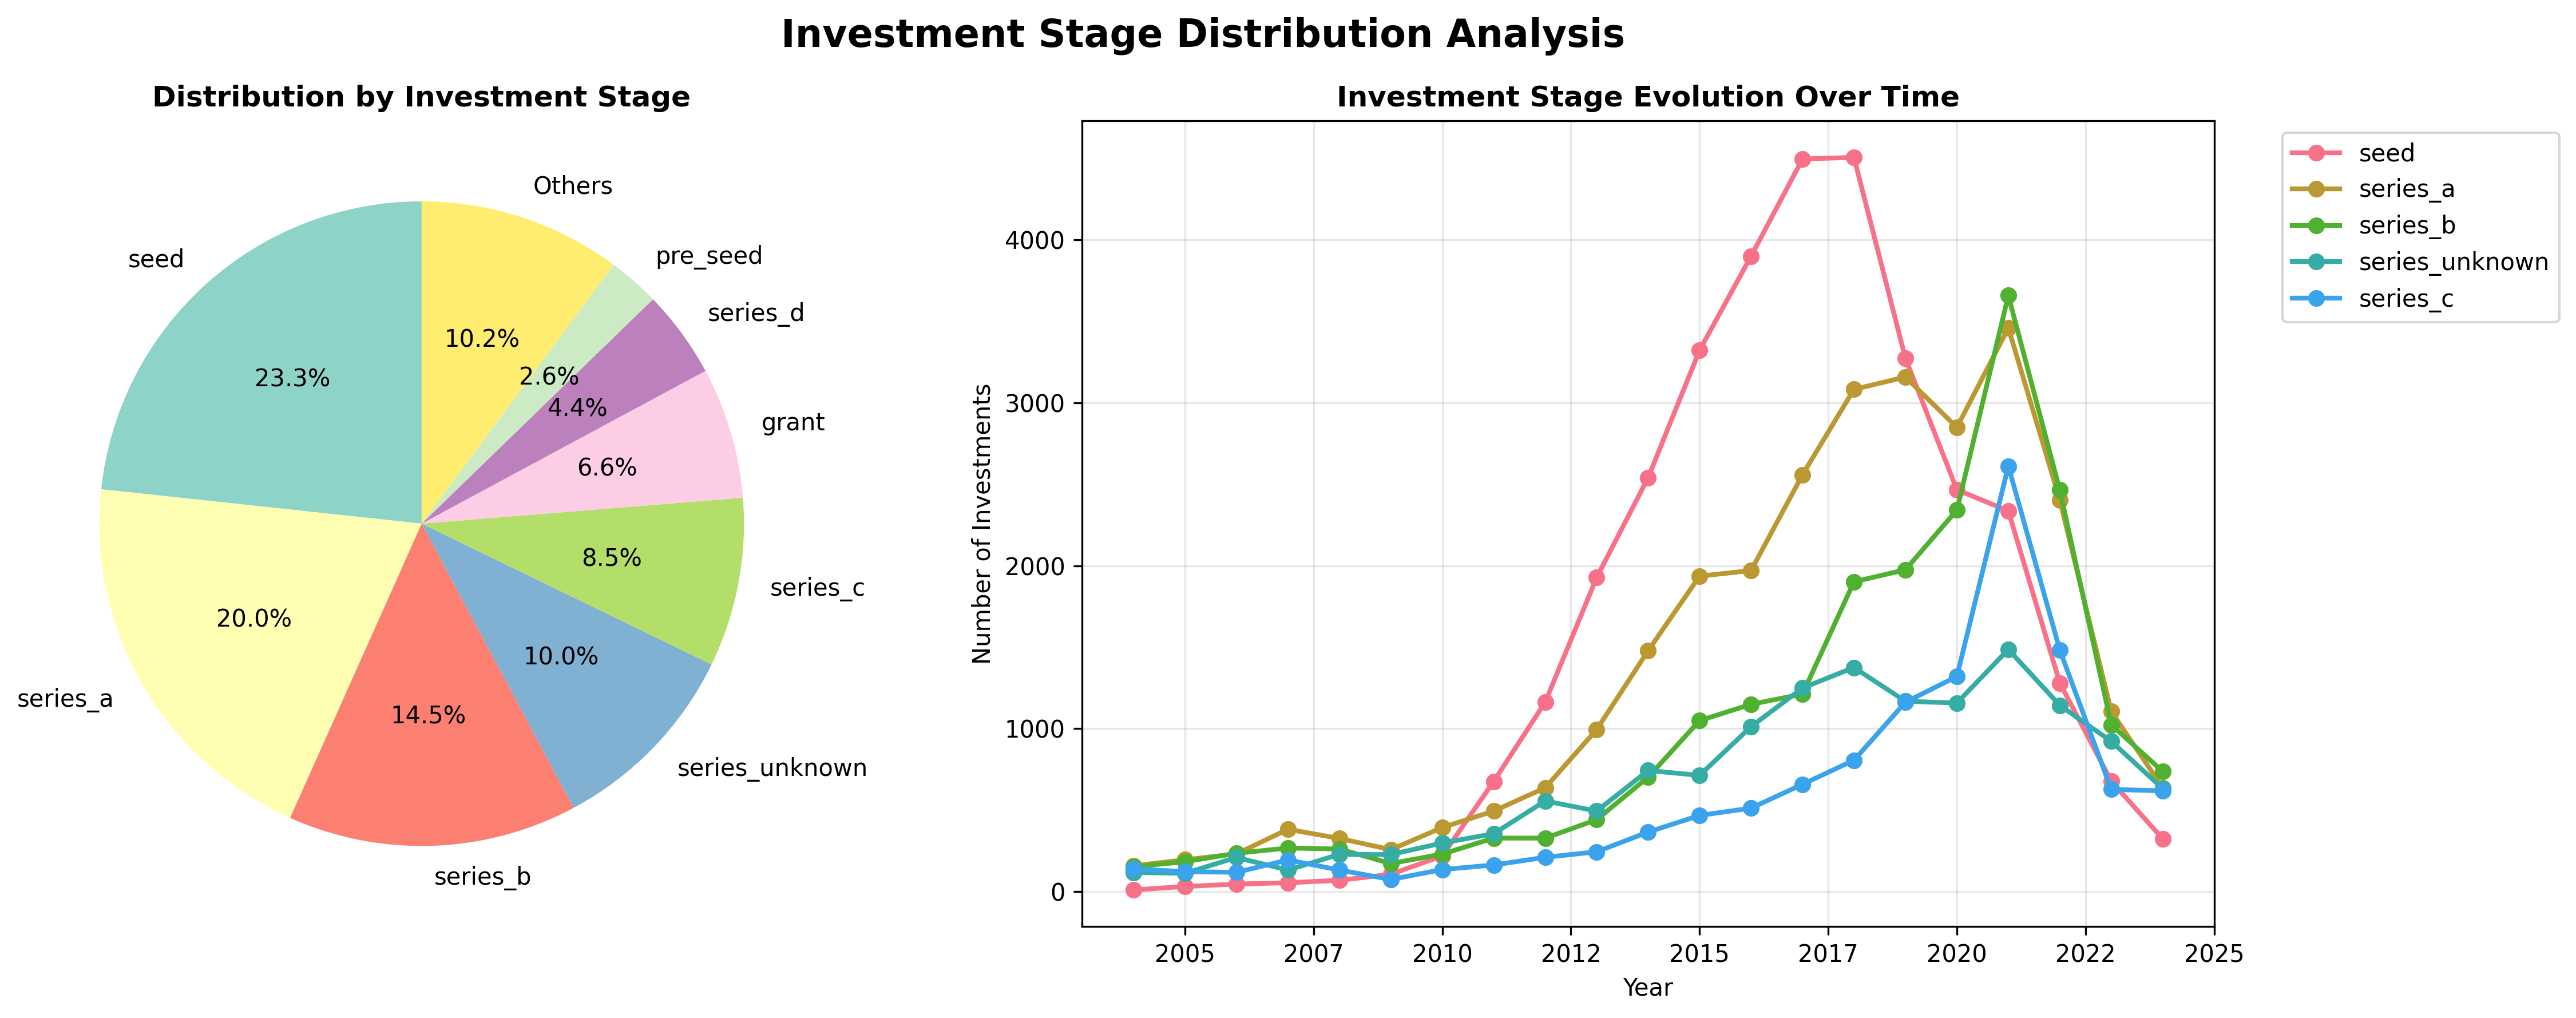
\includegraphics[width=1\textwidth]{../figures/us/investment_stage_distribution.png}
\caption{Distribution of investment stages across the venture capital dataset. The figure shows the prevalence of different funding stages, highlighting the concentration of activity in early-stage investments (seed and Series A) which together account for over 43\% of all transactions.}
\label{fig:investment_stage_dist}
\end{figure}

\begin{figure}[htbp]
\centering
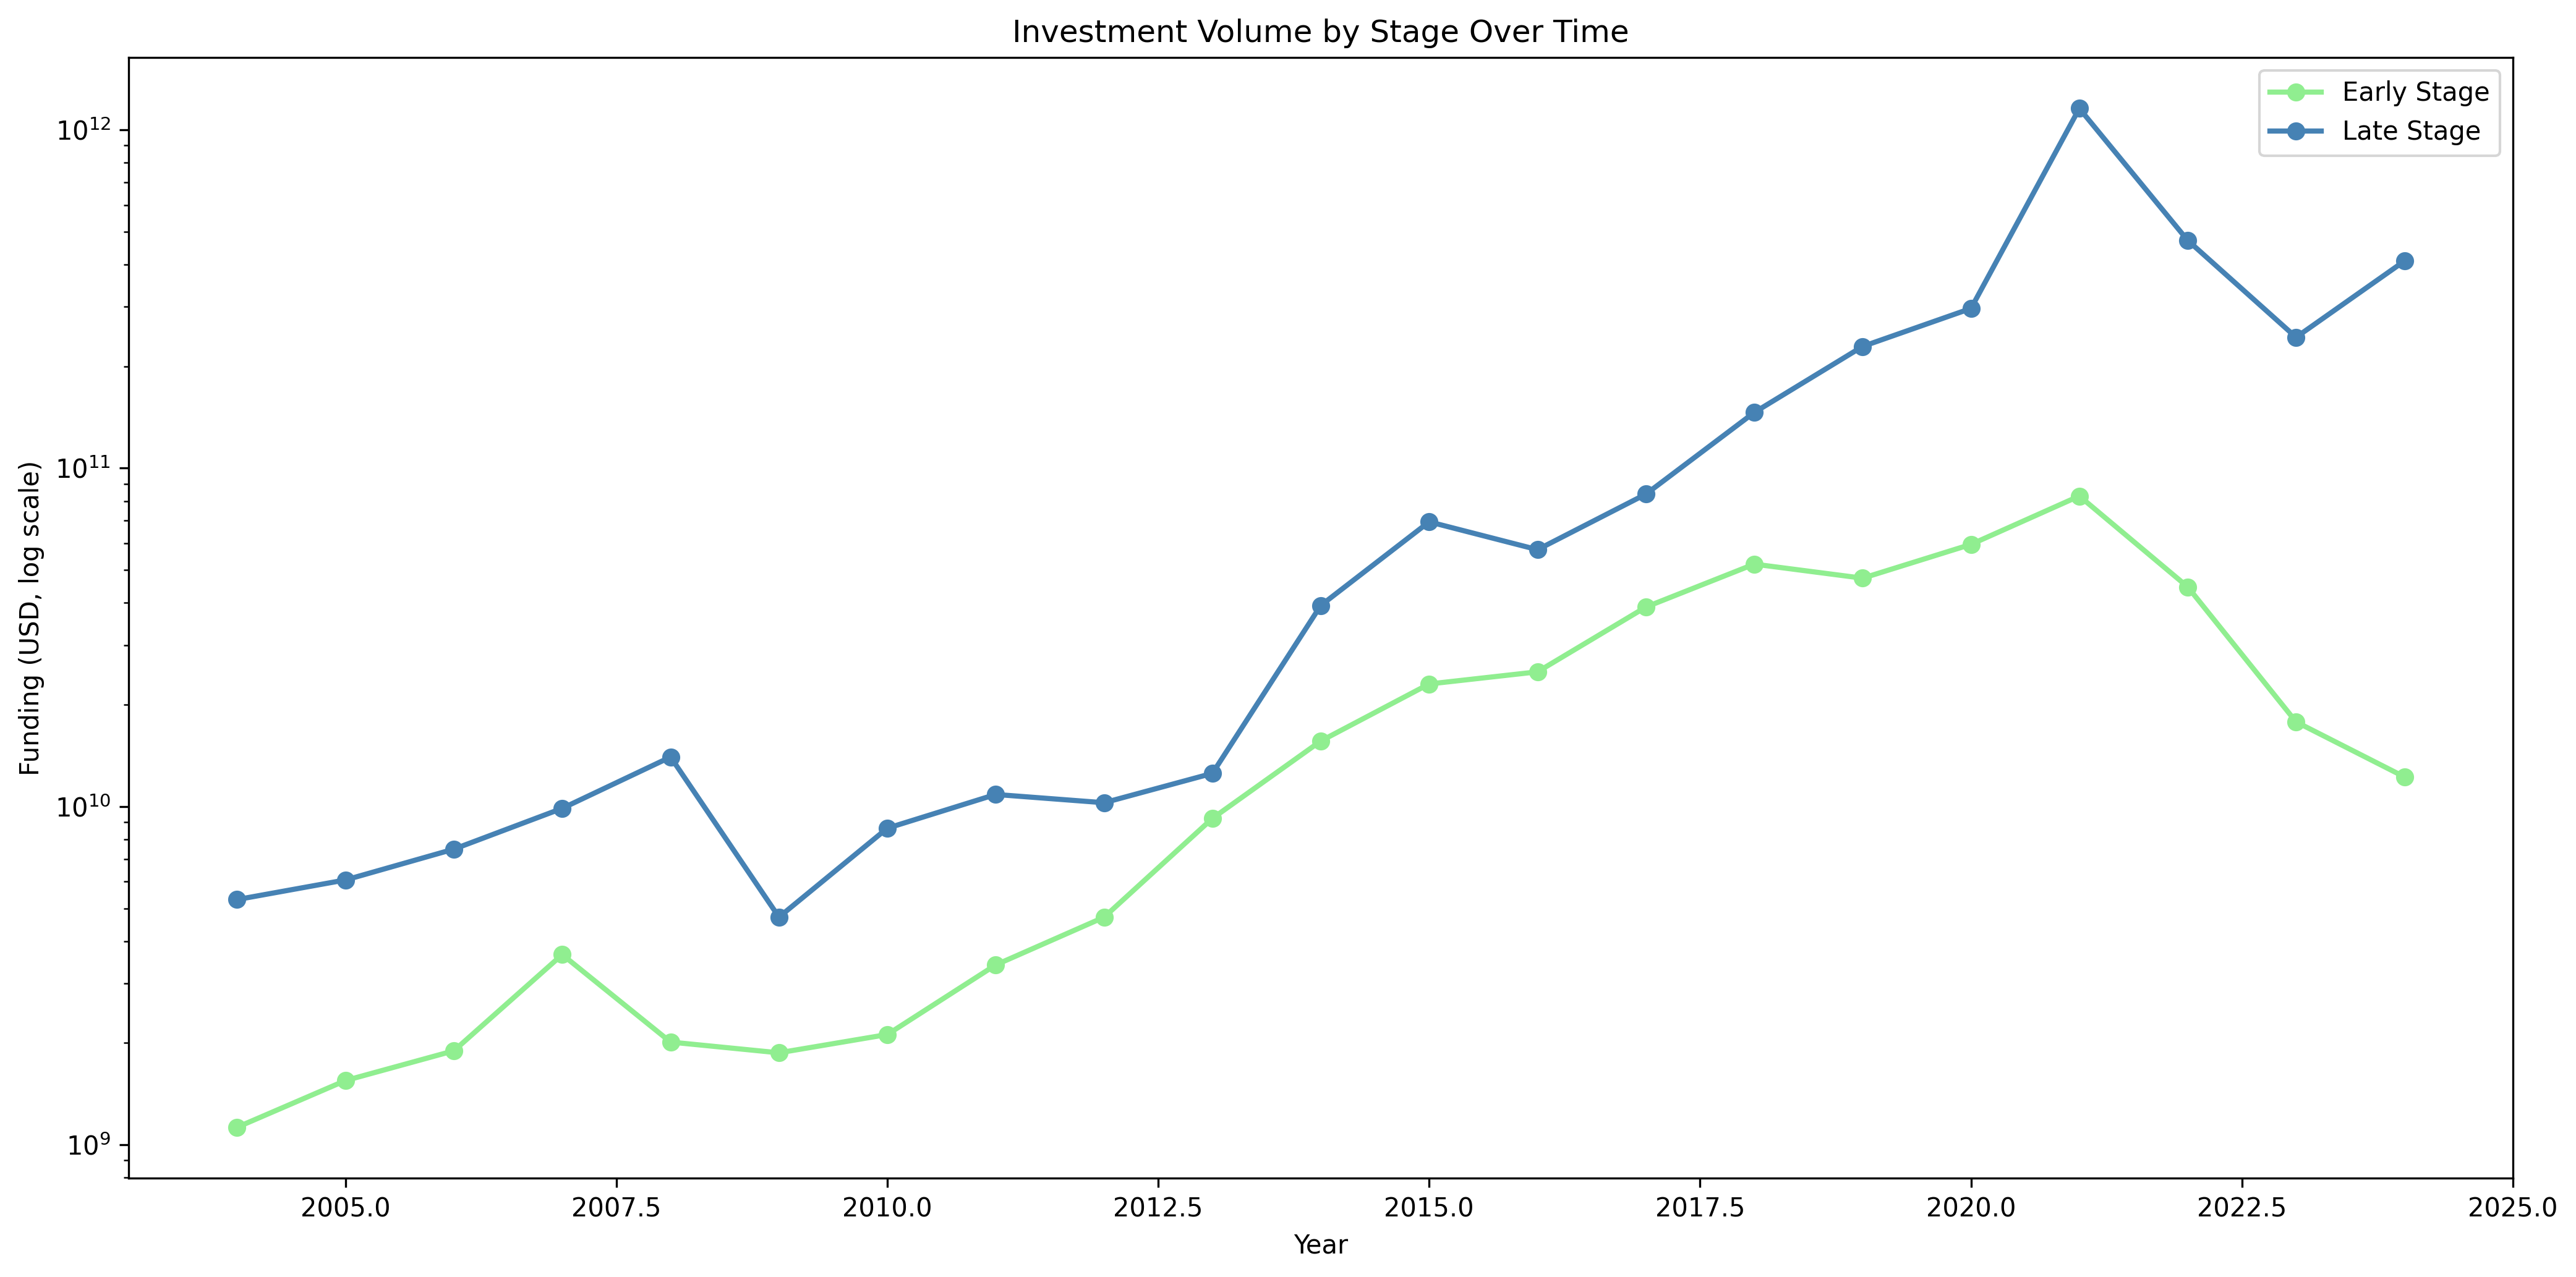
\includegraphics[width=1\textwidth]{../figures/us/investment_stage_curves_log.png}
\caption{Temporal evolution of investment stage distribution. This chart illustrates how the composition of different funding stages has evolved over time.}
\label{fig:investment_stage_temporal}
\end{figure}

The investment stage distribution demonstrates a clear early-stage focus within the venture capital ecosystem. Seed funding represents the largest single category at 23.3\% of all investments (33,419 transactions), followed closely by Series A at 20.0\% (28,703 transactions). This concentration in early-stage funding reflects the fundamental role of venture capital in supporting nascent companies during their most critical development phases.

When aggregated by stage classification, early-stage investments (angel through Series A) comprise 46.7\% of all transactions (66,978 investments), substantially exceeding late-stage investments (Series B and beyond) at 30.4\% (43,635 investments). The remaining 22.9\% consists of alternative funding mechanisms including grants, convertible notes, and specialized instruments.

However, temporal analysis also reveals a shift in capital allocation patterns. While early-stage investments dominate by transaction count, late-stage funding has achieved financial dominance in recent years. From 2004 to 2024, late-stage funding experienced exponential growth, escalating from \$5.31 billion in 2004 to \$409.52 billion in 2024 (a 77 times increase). In contrast, early-stage funding grew from \$1.13 billion to \$12.24 billion over the same period, representing an 11 times increase.

This divergence became particularly pronounced after 2013, when late-stage funding began substantially outpacing early-stage investments. By 2021, late-stage funding reached an unprecedented \$1.16 trillion, passing the \$82.74 billion in early-stage funding by a factor of 14. 

Even during the market correction of 2022-2024, late-stage funding maintained its dominance, suggesting a structural trend toward growth-stage capital deployment.

% The prevalence of Series B investments (14.5\%) as the dominant late-stage category by transaction count masks the reality that later-stage rounds involve substantially larger investment amounts. The declining percentages in subsequent series (C: 8.5\%, D: 4.4\%, E: 1.9\%) reflect both the increasingly selective nature of later-stage capital deployment and the substantially higher capital requirements of mature companies.

This capital concentration in late-stage investments may indicate the venture capital industry's evolution toward supporting unicorn creation and pre-IPO growth, where individual transactions can exceed hundreds of millions of dollars. The trend suggests that while early-stage investments remain crucial for company formation, the majority of venture capital deployment now focuses on scaling proven business models.

\todo{Some strong affirmatives need to have supporting references}

\subsubsection{Geographic Distribution}

As expected, as our dataset query was built to get US companies, the geographic distribution of venture capital investments reveals US-concentration pattern on global scale (Figure \ref{fig:geographic_distribution_country}). At US regional levels, Californian region (where Sylicon Valley is located) concentrates the invesment registers, as illustrated in Figure \ref{fig:geographic_distribution_region}.

\begin{figure}[htbp]
\centering
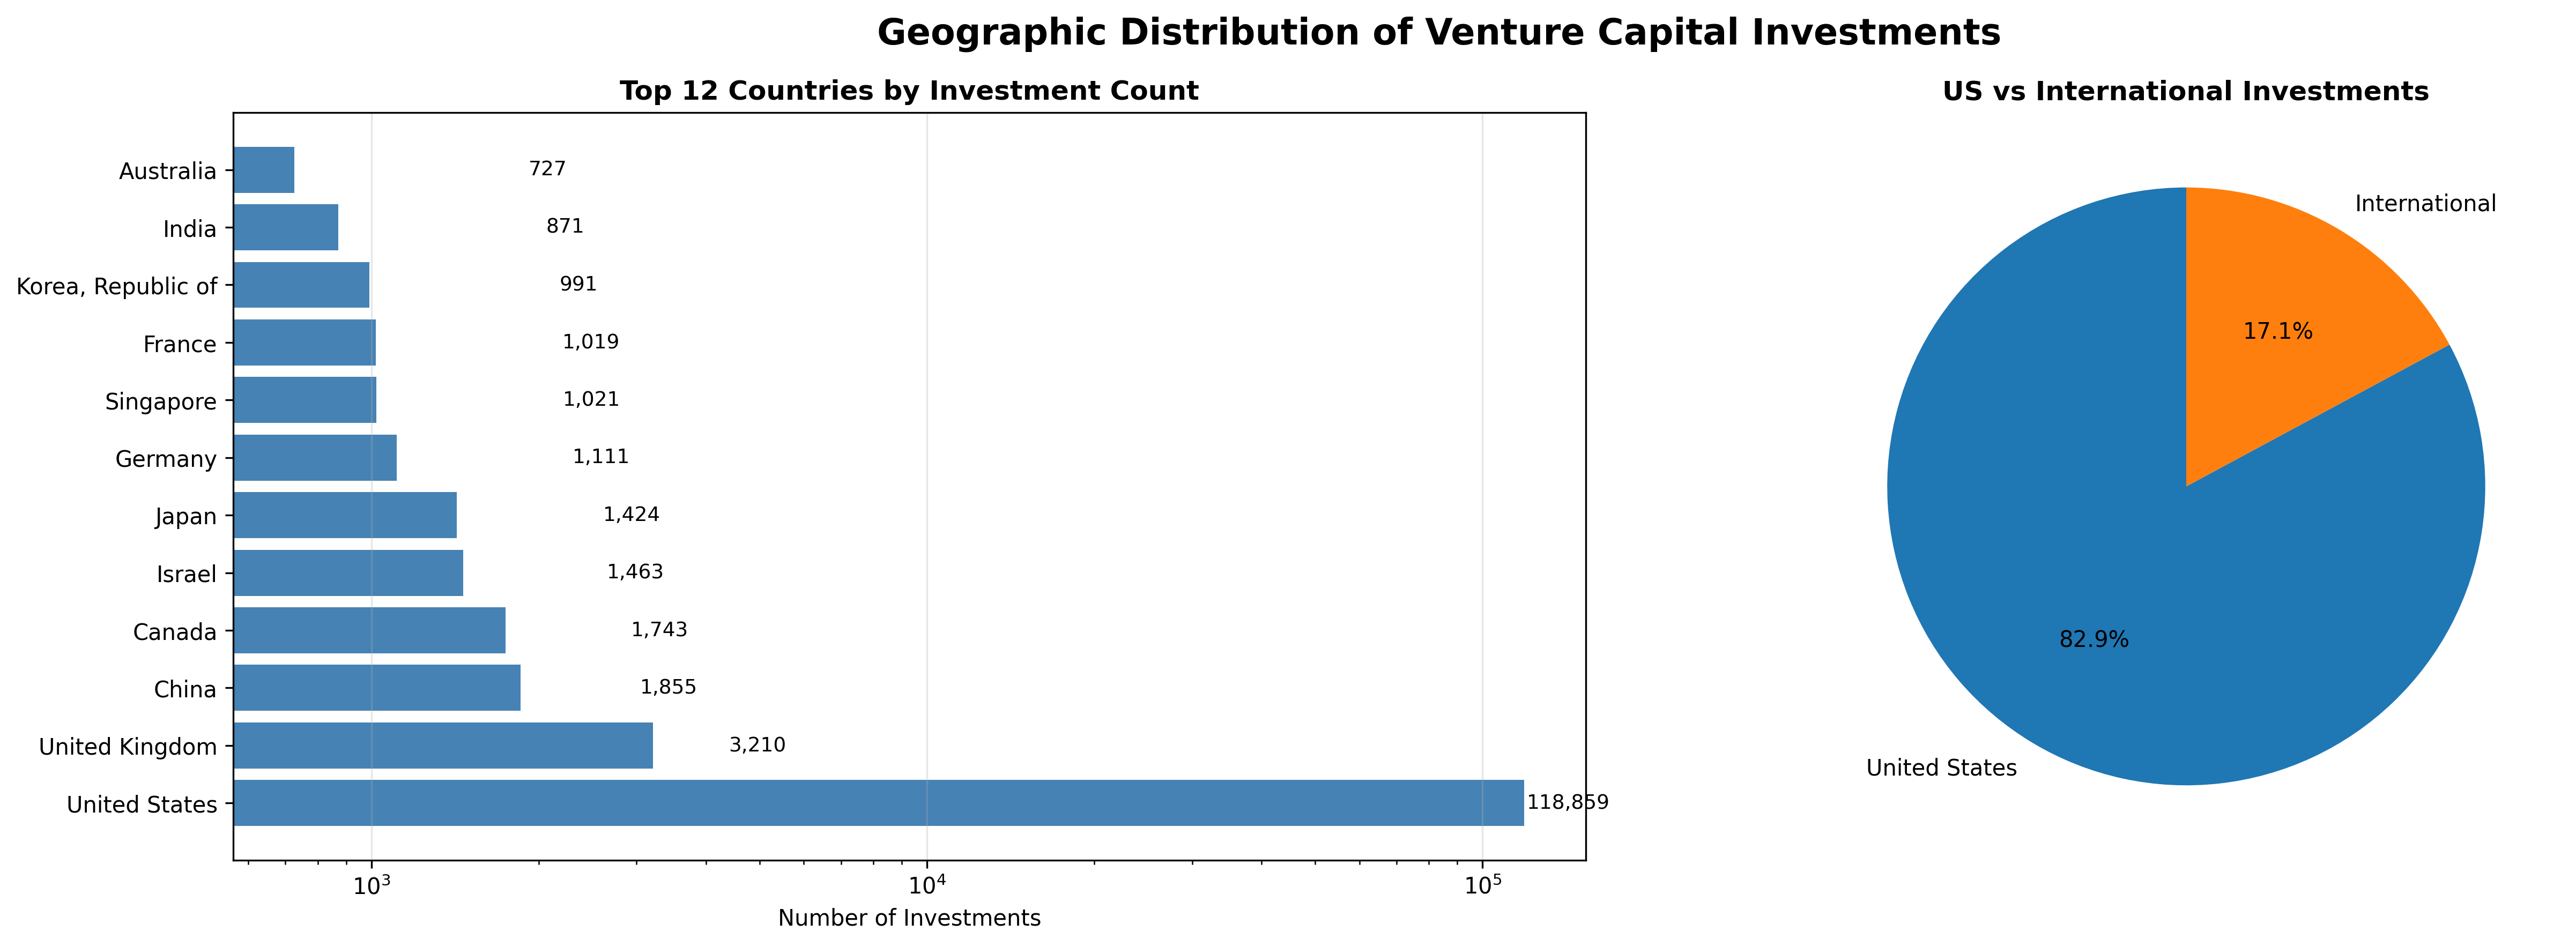
\includegraphics[width=1\textwidth]{../figures/us/geographic_distribution_country_analysis.png}
\caption{Geographic distribution of venture capital investments by country. The analysis shows the dominance of the United States VCs in venture capital activity on US (naturaly), accounting for 82.9\% of all investment transactions, with the top 15 countries representing the vast majority of global venture capital deployment on US.}
\label{fig:geographic_distribution_country}
\end{figure}

\begin{figure}[htbp]
\centering
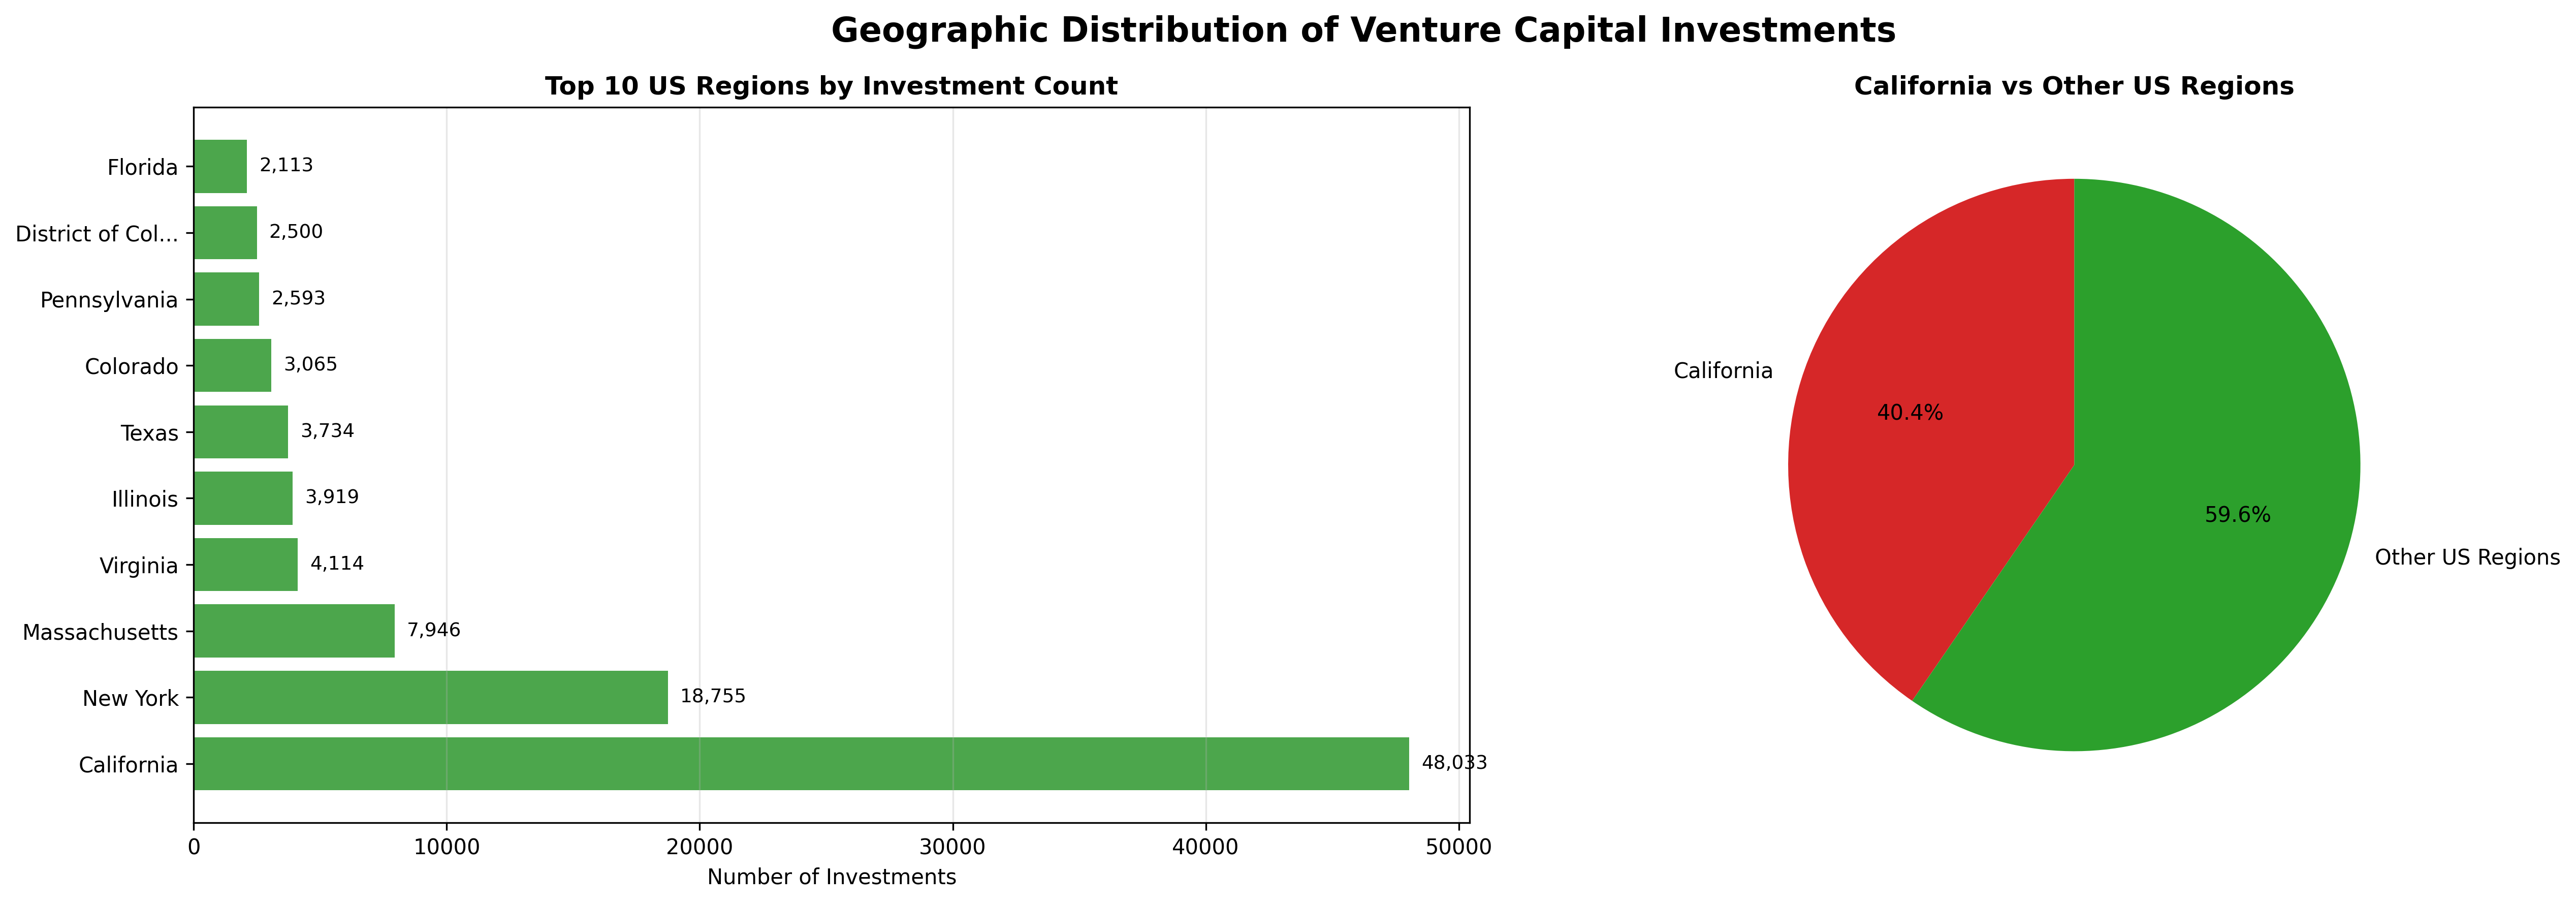
\includegraphics[width=1\textwidth]{../figures/us/geographic_distribution_region_analysis.png}
\caption{Regional distribution of venture capital investments within the United States. California emerges as the dominant hub with 40.4\% of all US investments, followed by New York at 15.8\%, demonstrating significant geographic clustering within the American venture capital ecosystem.}
\label{fig:geographic_distribution_region}
\end{figure}

Globally, the United States accounts for 118,859 investments (82.9\% of total activity), while international markets collectively represent 24,579 investments (17.1\%). Among international markets, the United Kingdom leads with 3,210 investments (2.2\%), followed by China with 1,855 investments (1.3\%) and Canada with 1,743 investments (1.2\%).

Within the United States, regional concentration patterns mirror the global trend. California dominates with 48,033 investments (40.4\% of US total), representing nearly half of all American venture capital activity. New York follows as the second-largest market with 18,755 investments (15.8\%), while Massachusetts ranks third with 7,946 investments (6.7\%). The top ten US regions account for approximately 81.5\% of all domestic venture capital transactions.

These geographic patterns reflect the clustering effects of venture capital ecosystems around established technology and financial centers. The concentration in California, particularly in Silicon Valley, and New York's financial district demonstrates how proximity to talent, infrastructure, and capital sources influences investment distribution. Similar clustering patterns emerge internationally, with London, Beijing, and Toronto serving as regional venture capital hubs for funds coming to US.

\subsubsection{Sectorial Distribution}

The sectoral distribution analysis reveals significant concentration patterns in venture capital investment activity. As illustrated in Figure \ref{fig:sectoral_industry_bars}, health care dominates the investment landscape with 21,574 investments (15.0\% of total activity), followed by financial services at 11,409 investments (8.0\%) and data and analytics at 8,626 investments (6.0\%).

\begin{figure}[htbp]
\centering
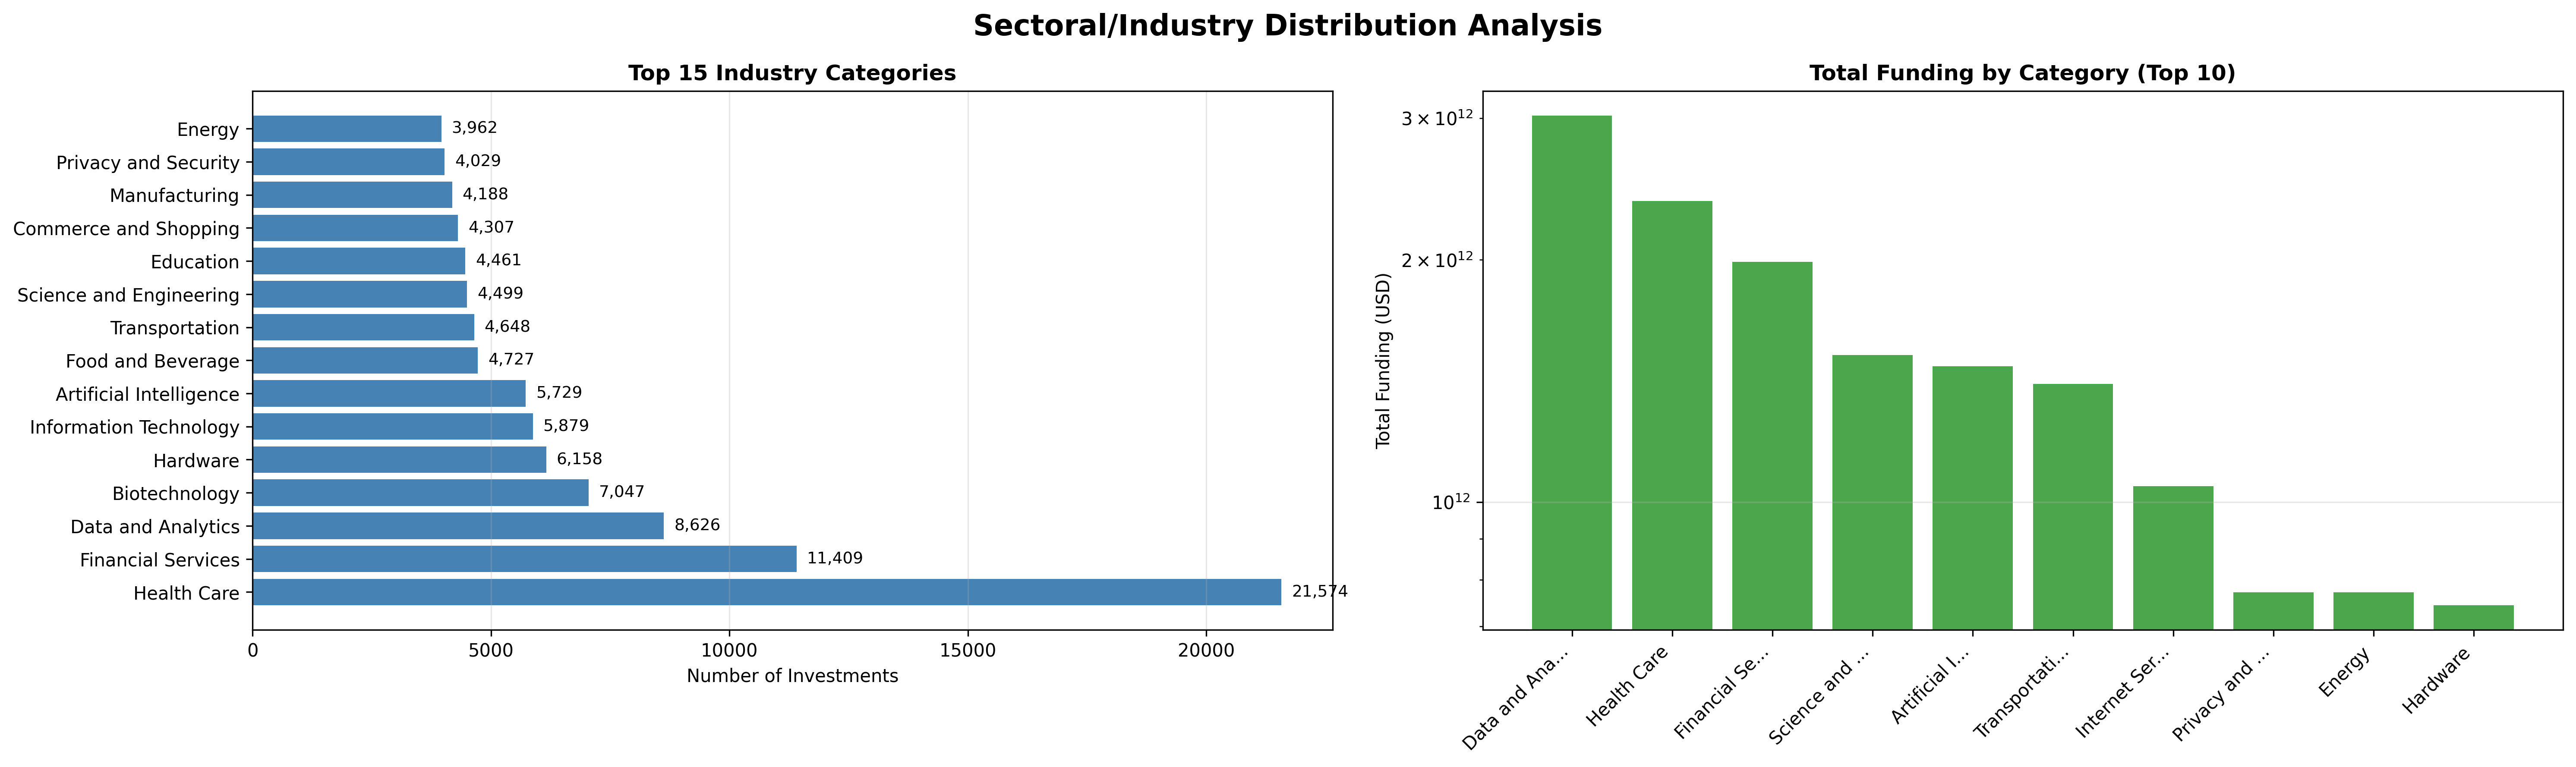
\includegraphics[width=1\textwidth]{../figures/us/sectoral_industry_analysis_bars.png}
\caption{Sectoral distribution of venture capital investments across industry categories. The bar chart shows the concentration of investment activity, with health care as the dominant sector, followed by financial services and data analytics. The top 20 categories account for over 81\% of all investment transactions.}
\label{fig:sectoral_industry_bars}
\end{figure}

The investment concentration demonstrates a highly uneven distribution across sectors. The top 5 categories capture 38.2\% of total investments, while the top 10 categories account for 56.0\% of all activity. This concentration extends to the top 20 categories, which represent 81.2\% of total investments across only 42 unique industry categories.

Technology-related sectors represent a notable but minority portion of the ecosystem. The analysis identifies 6 technology categories (artificial intelligence, data and analytics, hardware, information technology, privacy and security, and internet services) that collectively account for 33,998 investments (23.7\% of total activity). The remaining 109,440 investments (76.3\%) occur in non-technology sectors, indicating that venture capital deployment extends well beyond traditional technology boundaries.

Figure \ref{fig:sectoral_industry_trends} illustrates the temporal evolution of sectoral investment patterns, revealing how industry preferences have shifted over time.

\begin{figure}[htbp]
\centering
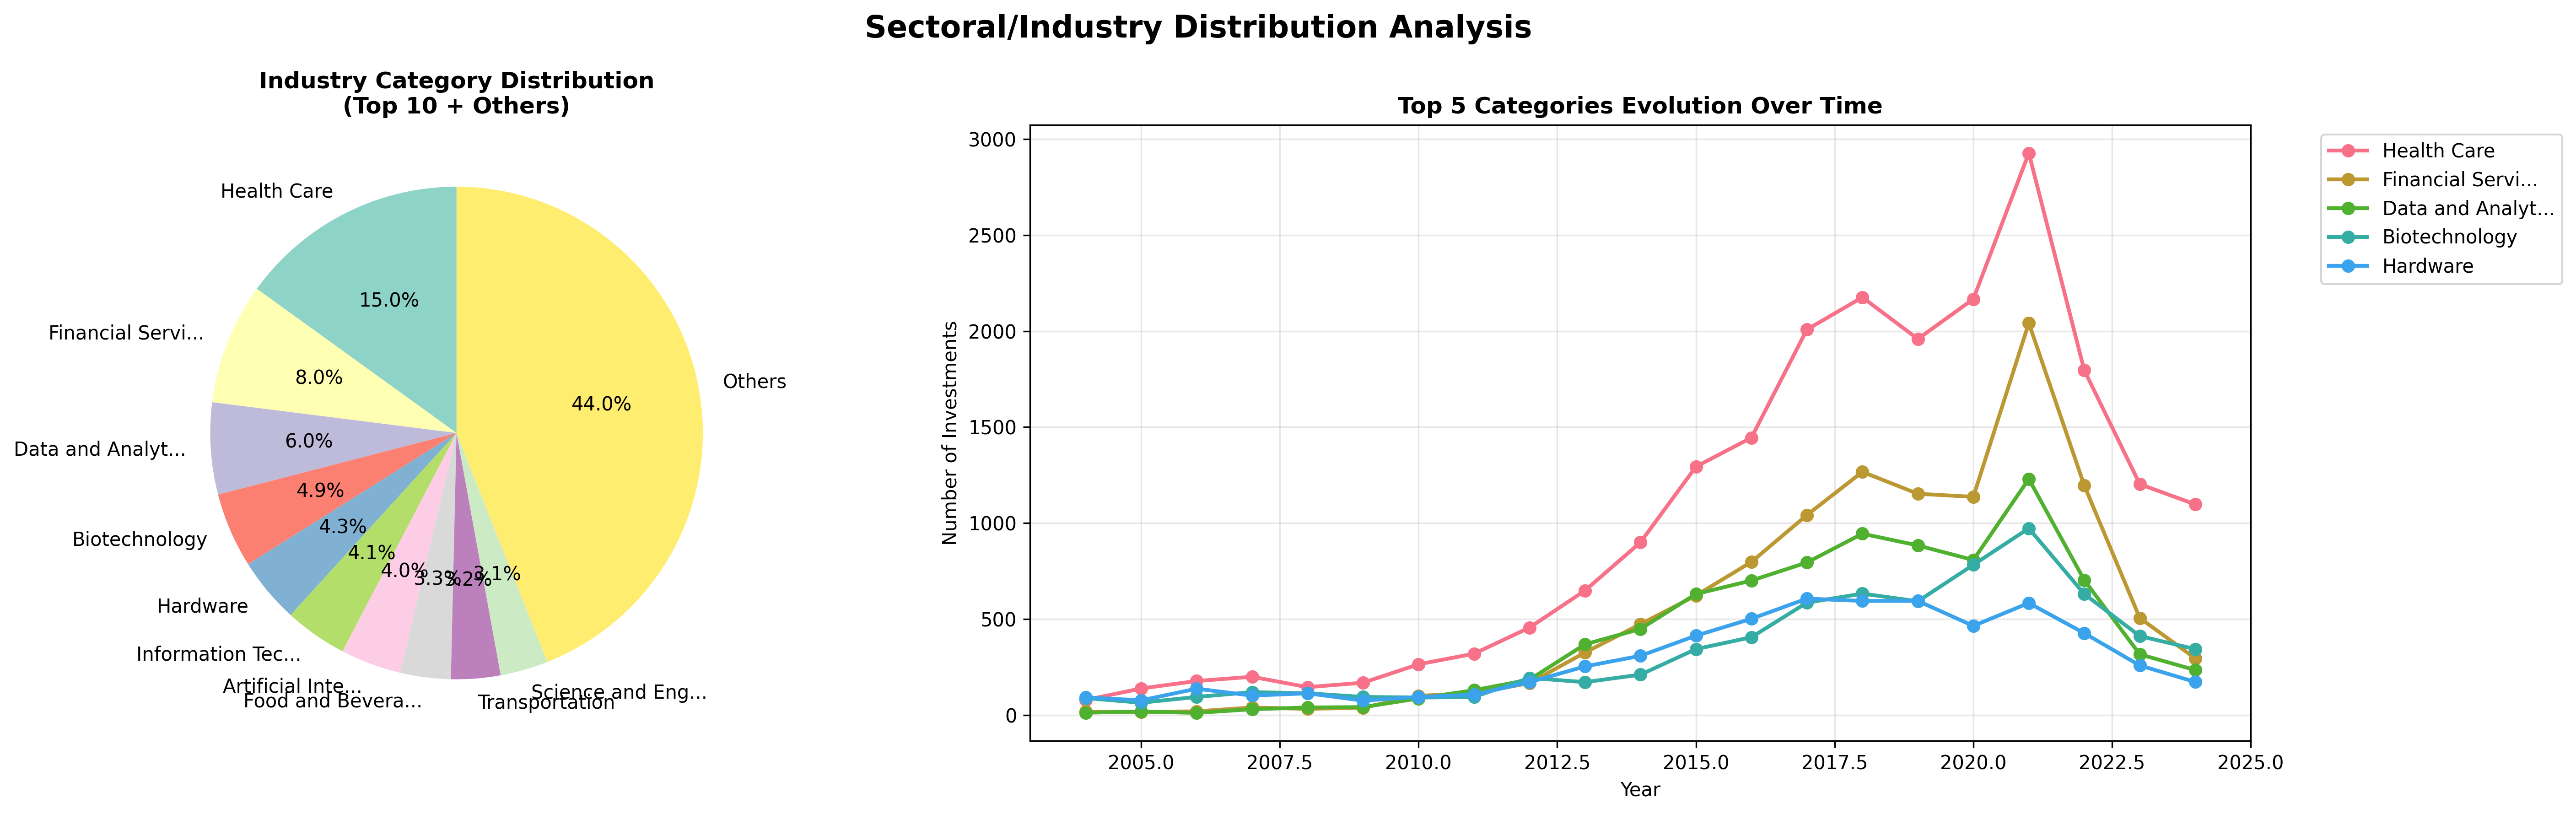
\includegraphics[width=1\textwidth]{../figures/us/sectoral_industry_analysis_trends.png}
\caption{Temporal trends in sectoral investment distribution. The figure shows how investment patterns across different industry categories have evolved over time, highlighting the growth trajectories of major sectors and the emergence of new investment areas.}
\label{fig:sectoral_industry_trends}
\end{figure}

The healthcare sector's dominance reflects the substantial capital requirements and long development cycles characteristic of medical innovation, which align well with venture capital investment strategies. Financial services' strong showing demonstrates the ongoing fintech revolution and the digitization of traditional financial institutions.

The presence of traditional sectors like food and beverage (4,727 investments, 3.3\%), transportation (4,648 investments, 3.2\%), and manufacturing (4,188 investments, 2.9\%) among the top categories indicates that venture capital has expanded beyond its historical technology focus to encompass a broader range of innovation-driven industries.

Biotechnology's position as the fourth-largest category (7,047 investments, 4.9\%) highlights the significant role of life sciences in the venture capital ecosystem, often requiring specialized knowledge and longer investment horizons compared to other sectors.

\subsection{Communities Characterization}

\newcommand{\invPairs}{169,679}
\newcommand{\invPairsUniqueStartups}{3,666}

The division of venture capital firms into early-stage and late-stage investor groups results in \invPairs{} investment pairs comprising \invPairsUniqueStartups{} unique startups.

\newcommand{\numCommunities}{168}
\newcommand{\numTopCommunities}{5}
\newcommand{\numCommunitiesThreshold}{150}

Community detection using greedy modularity optimization identifies approximately \numCommunities{} distinct communities (the number of communities oscillates between 167 and 175 across different trials), with the largest communities containing over 4000 investors each, followed by 1 community with almost 1000 agents, 4 communities with more than 100 agents, and then several smaller groups, as summarized in Table~\ref{tab:community_sizes}.

Initially, analysis focuses on communities with at least \numCommunitiesThreshold{} nodes to ensure statistical power for nestedness analysis. This threshold yields \numTopCommunities{} communities.

\todo[inline]{Add rationale for threshold}

\begin{table}[htp]
\centering
\begin{tabular}{|c|c|}
\hline
\textbf{Community ID} & \textbf{Number of Investors} \\
\hline
0 & 4,248 \\
1 & 4,089 \\
2 & 3,959 \\
3 & 979 \\
4 & 188 \\
5 & 155 \\
6 & 137 \\
7 & 122 \\
\hline
\end{tabular}
\caption{Size distribution of the largest investor communities identified through greedy modularity optimization}
\label{tab:community_sizes}
\end{table}

The largest three communities (0, 1, and 2) contain over 12,000 investors combined, representing approximately 75\% of all investors in the network. This concentration suggests a highly centralized structure within the venture capital ecosystem, with most investment activity occurring within a small number of large communities, what suggests community size distribution follows a typical power-law pattern observed in many social networks \cite{Borgatti2011}. 

\todo[inline]{Mention literature, as this phenomenon is well-documented}

\todo[inline]{Add figure of community size distribution}

Community boundaries are defined at the node level, meaning each investor belongs to exactly one community. However, edges (investment relationships) can span community boundaries when investors from different communities co-invest in the same startup.

To analyze investment patterns, we classify each syndicated investment as either: (1) intra-community if all participating investors belong to the same community, or (2) cross-community if investors from multiple communities participate together. Table \ref{tab:investment_distribution} presents the resulting investment distribution across communities.

\begin{table}[htbp]
\centering
\begin{tabular}{|c|c|c|}
\hline
\textbf{Community} & \textbf{Co-investments Pairs} & \textbf{Relative Proportion} \\
\hline
Community 0 & 32,164 & 19.4\% \\
Community 1 & 17,301 & 10.4\% \\
Community 2 & 55,863 & 33.6\% \\
Cross-community & 58,329 & 35.1\% \\
\hline
\end{tabular}
\caption{Distribution of syndicated investments across investor communities}
\label{tab:investment_distribution}
\end{table}

The analysis reveals important patterns in investment activity distribution. Community 2 accounts for the largest share of investments (33.6\%), containing approximately 50\% more investments than Community 0 and over three times more than Community 1. This concentration of investment activity suggests that structural features of Community 2 may facilitate higher transaction volumes. Notably, cross-community investments represent over one-third of all transactions, indicating substantial interconnectedness across community boundaries.

\subsubsection{Degree Distribution}

Before further examining community-level investment patterns in-depth, we analyze the degree distribution characteristics across the three largest investor communities. This analysis reveals that all communities exhibit power-law patterns typical of scale-free networks, with notable differences in magnitude and scale parameters.

Communities 0 and 2 demonstrate remarkably similar degree distribution magnitudes, while Community 1 exhibits consistently lower magnitude values across all degree ranges. This pattern becomes particularly evident when examining the degree distributions on a logarithmic scale, where Community 2 shows the highest volume of nodes across all degree ranges, suggesting greater overall connectivity within this community.

\todo[inline]{Compare connectance among communities}

\begin{figure}[ht]
\centering
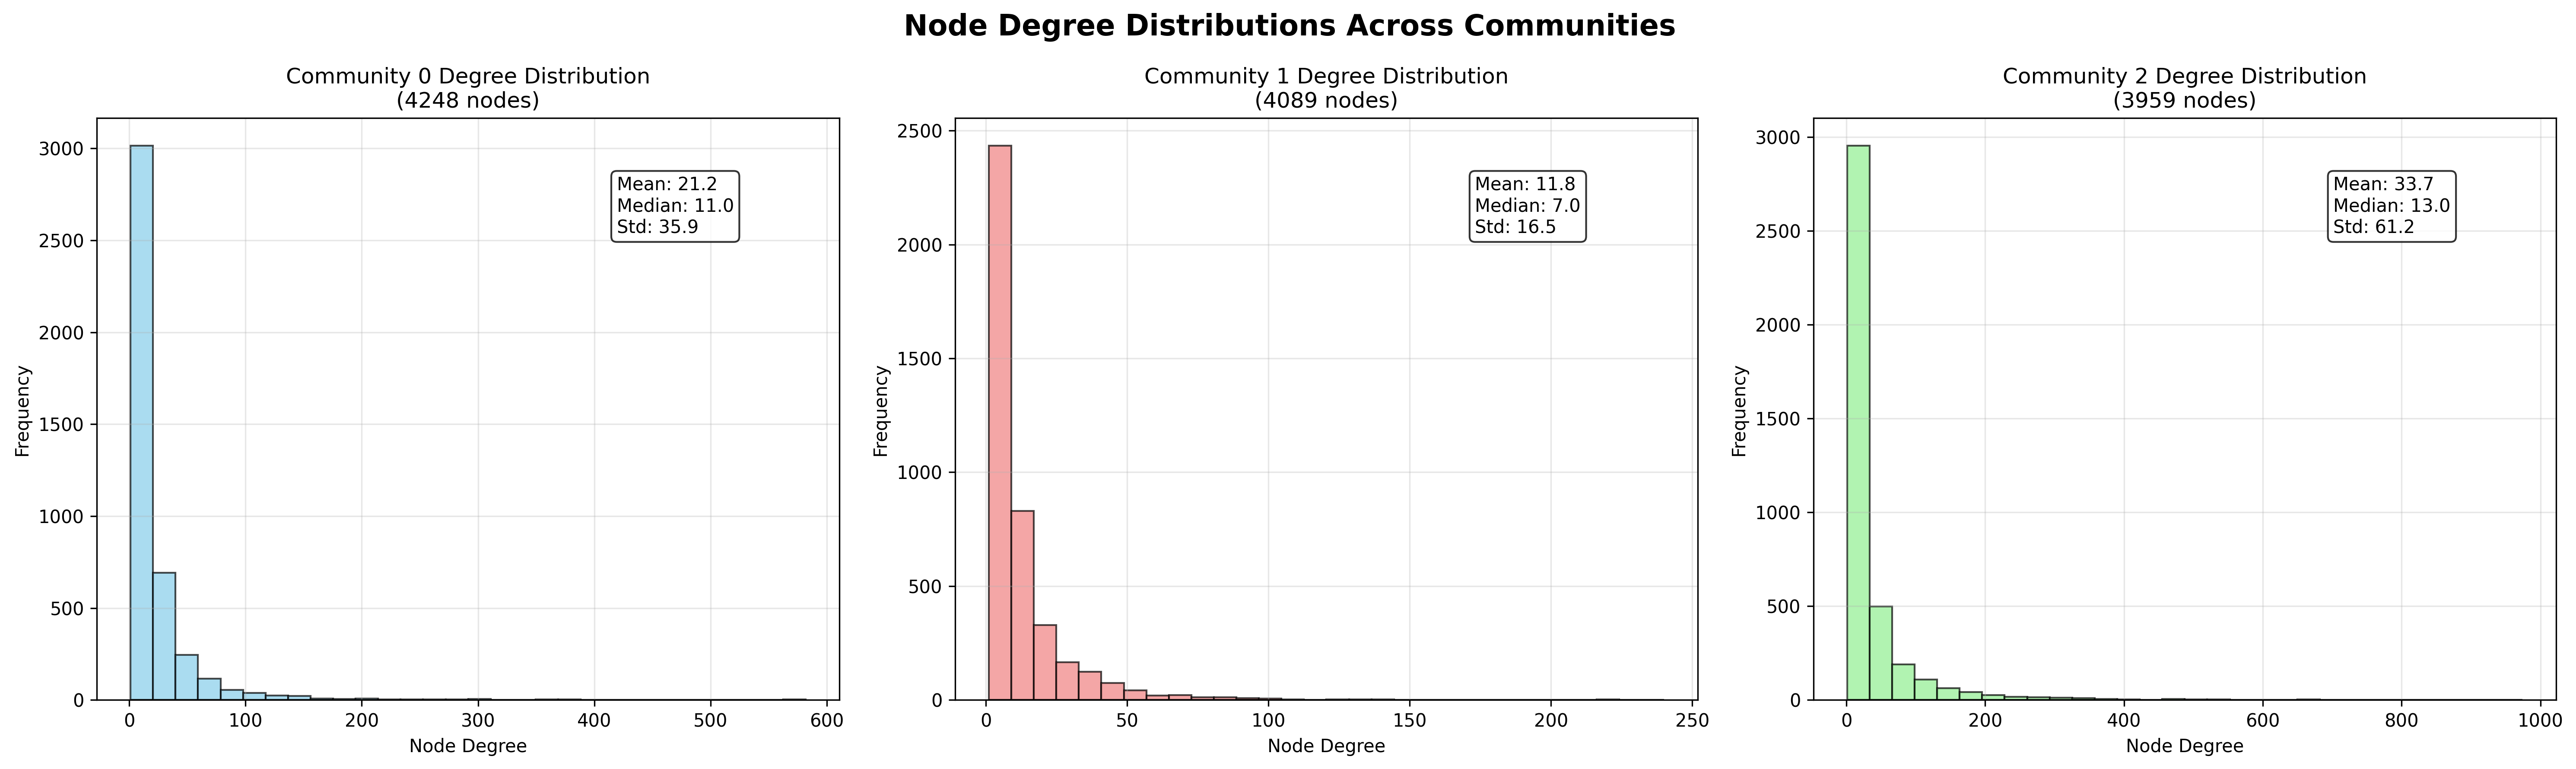
\includegraphics[width=1\textwidth]{../figures/us/node_degree_distributions_comprehensive_pt1.png}
\caption{Node degree distributions for the three largest investor communities. The figure shows both the individual degree distributions and their overlap on a logarithmic scale. Communities 0 and 2 display similar heavy-tailed, power-law-like patterns, while Community 1 has consistently lower degree magnitudes. The log-scale overlay highlights that Community 2 maintains the highest node volume across all degree ranges, indicating greater overall connectivity.}
\label{fig:node_degree_distributions}
\end{figure}

\begin{figure}[ht]
\centering
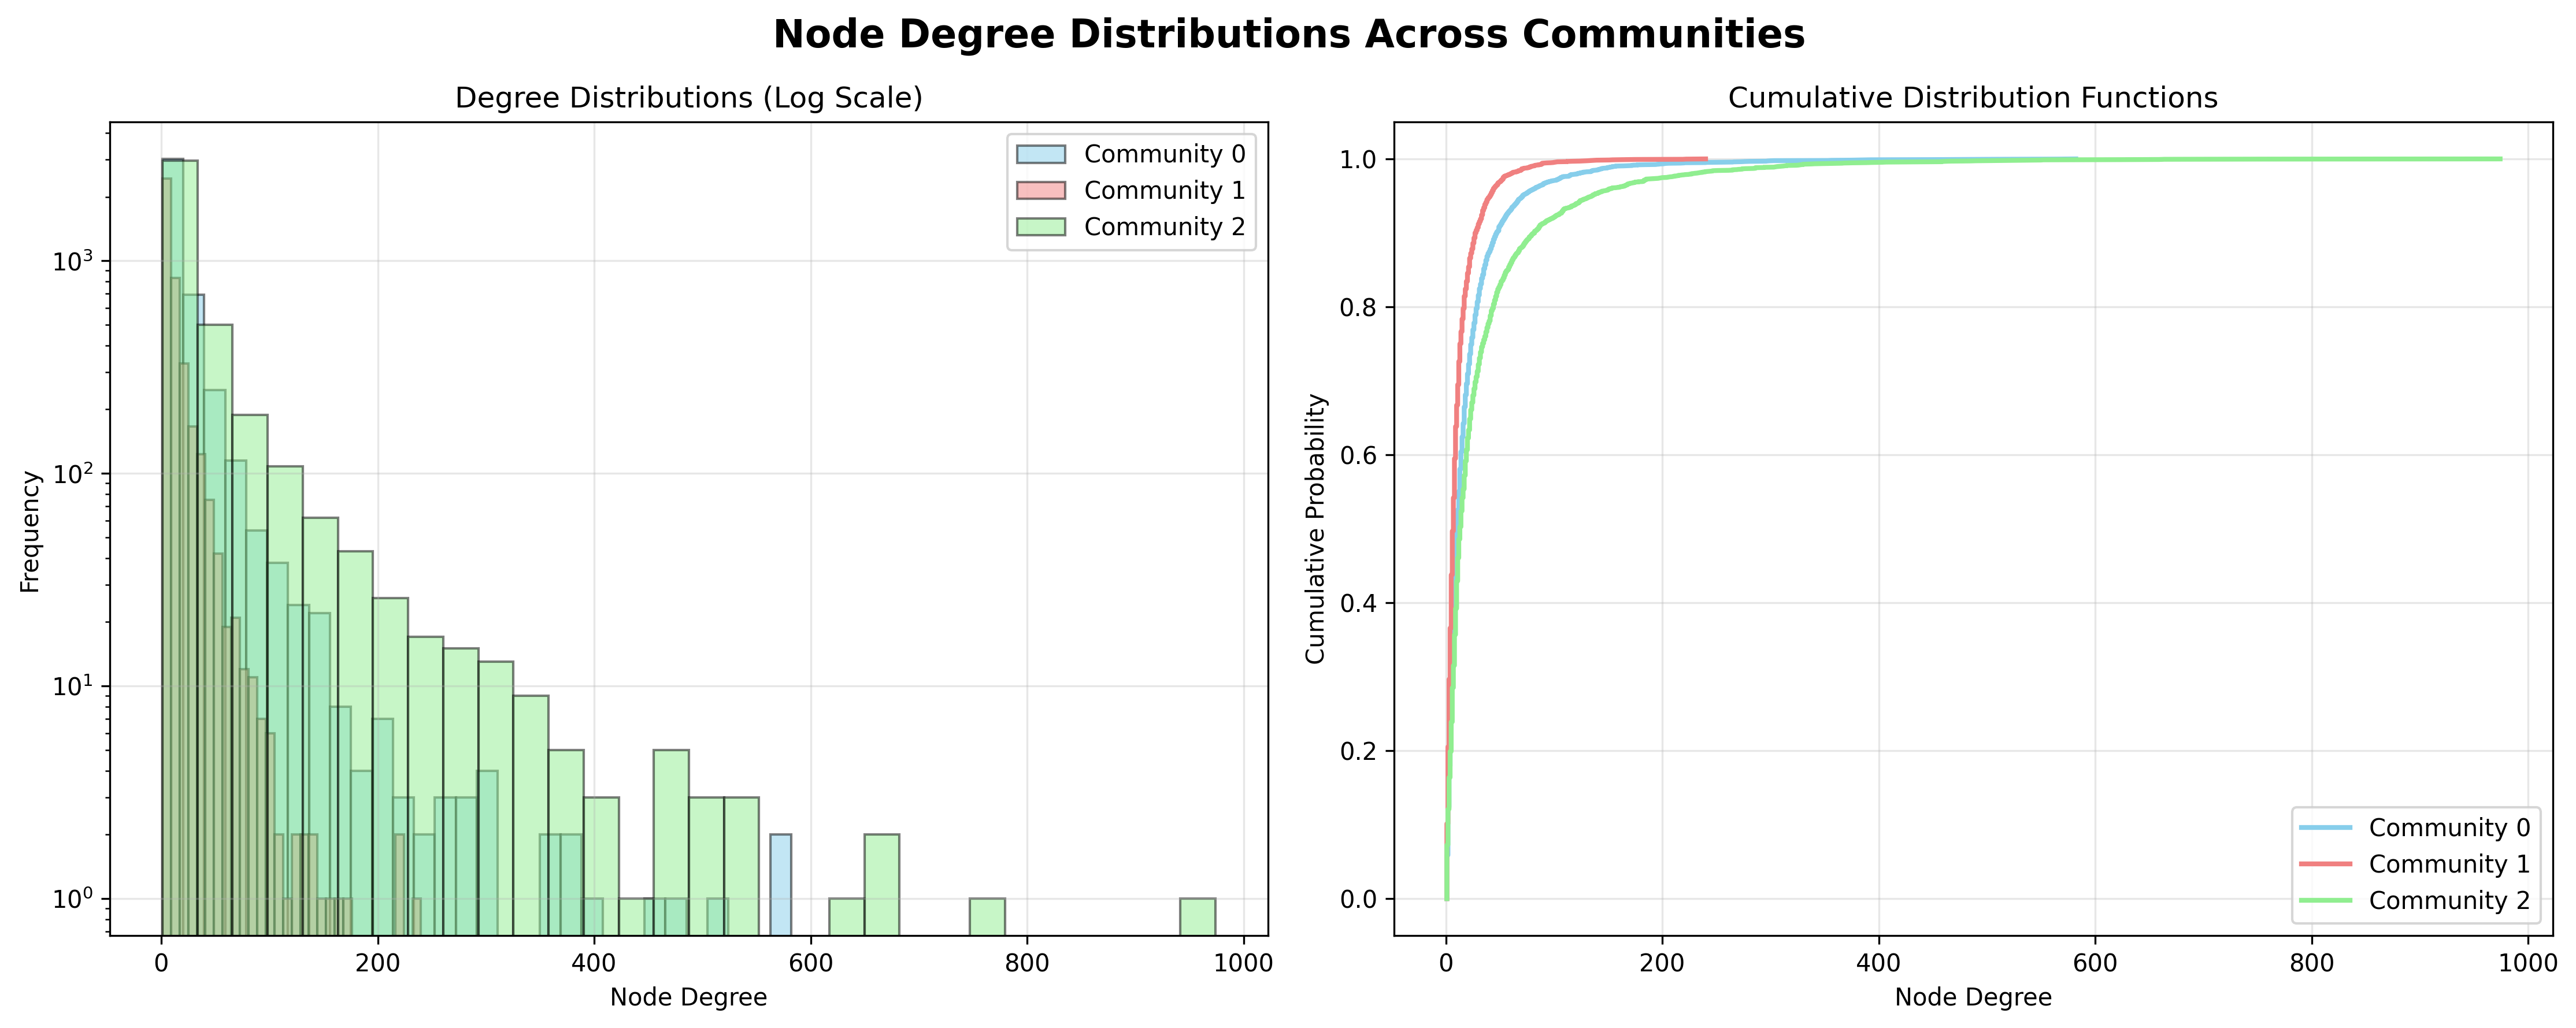
\includegraphics[width=1\textwidth]{../figures/us/node_degree_distributions_comprehensive_pt2.png}
\caption{TBD}
\label{fig:node_degree_distributions}
\end{figure}

Analysis of high-degree nodes (95th percentile) reveals distinct patterns across communities. Community 0 demonstrates a mixed composition of hub nodes, with early-stage investors like Techstars-seed (degree: 582) and 500 Global-seed (degree: 564) dominating the highest positions, alongside significant late-stage players such as Gaingels-series\_b (degree: 509). 

Community 1 exhibits a more balanced distribution with Intel Capital maintaining strong presence across multiple investment stages, while Community 2 shows remarkable concentration among early-stage Silicon Valley investors, with SV Angel-seed achieving the highest connectivity (degree: 974) followed by other prominent early-stage firms including Andreessen Horowitz and Khosla Ventures.

Table \ref{tab:high_degree_nodes} presents the top high-degree nodes for each community, highlighting the structural differences in hub organization.

\begin{table}[ht]
\centering
\begin{tabular}{|c|l|c|c|}
\hline
\textbf{Community} & \textbf{Investor} & \textbf{Degree} & \textbf{Type} \\
\hline
\multirow{5}{*}{0} & Techstars-seed & 582 & Early-stage \\
& 500 Global-seed & 564 & Early-stage \\
& Gaingels-series\_b & 509 & Late-stage \\
& Greycroft-series\_a & 483 & Early-stage \\
& Bossa Invest-series\_b & 450 & Late-stage \\
\hline
\multirow{5}{*}{1} & Intel Capital-series\_b & 240 & Late-stage \\
& Norwest Venture Partners-series\_a & 222 & Early-stage \\
& Canaan Partners-series\_a & 219 & Early-stage \\
& Intel Capital-series\_c & 175 & Late-stage \\
& SOSV-series\_b & 163 & Late-stage \\
\hline
\multirow{5}{*}{2} & SV Angel-seed & 974 & Early-stage \\
& SV Angel-series\_a & 754 & Early-stage \\
& Andreessen Horowitz-series\_a & 664 & Early-stage \\
& Khosla Ventures-series\_a & 659 & Early-stage \\
& New Enterprise Associates-series\_a & 619 & Early-stage \\
\hline
\end{tabular}
\caption{Top 5 high-degree nodes (95th percentile) for the three largest investor communities}
\label{tab:high_degree_nodes}
\end{table}

As per Figure \ref{fig:degree_vs_activity}, the relationship between degree centrality and investment activity demonstrates a positive correlation across all communities, with higher-degree nodes exhibiting greater investment frequency. This pattern suggests that network position, as measured by degree centrality, serves as a reliable predictor of investment activity levels within the venture capital ecosystem.

\todo[inline]{Add more centrality metrics}

\begin{figure}[htpb]
\centering
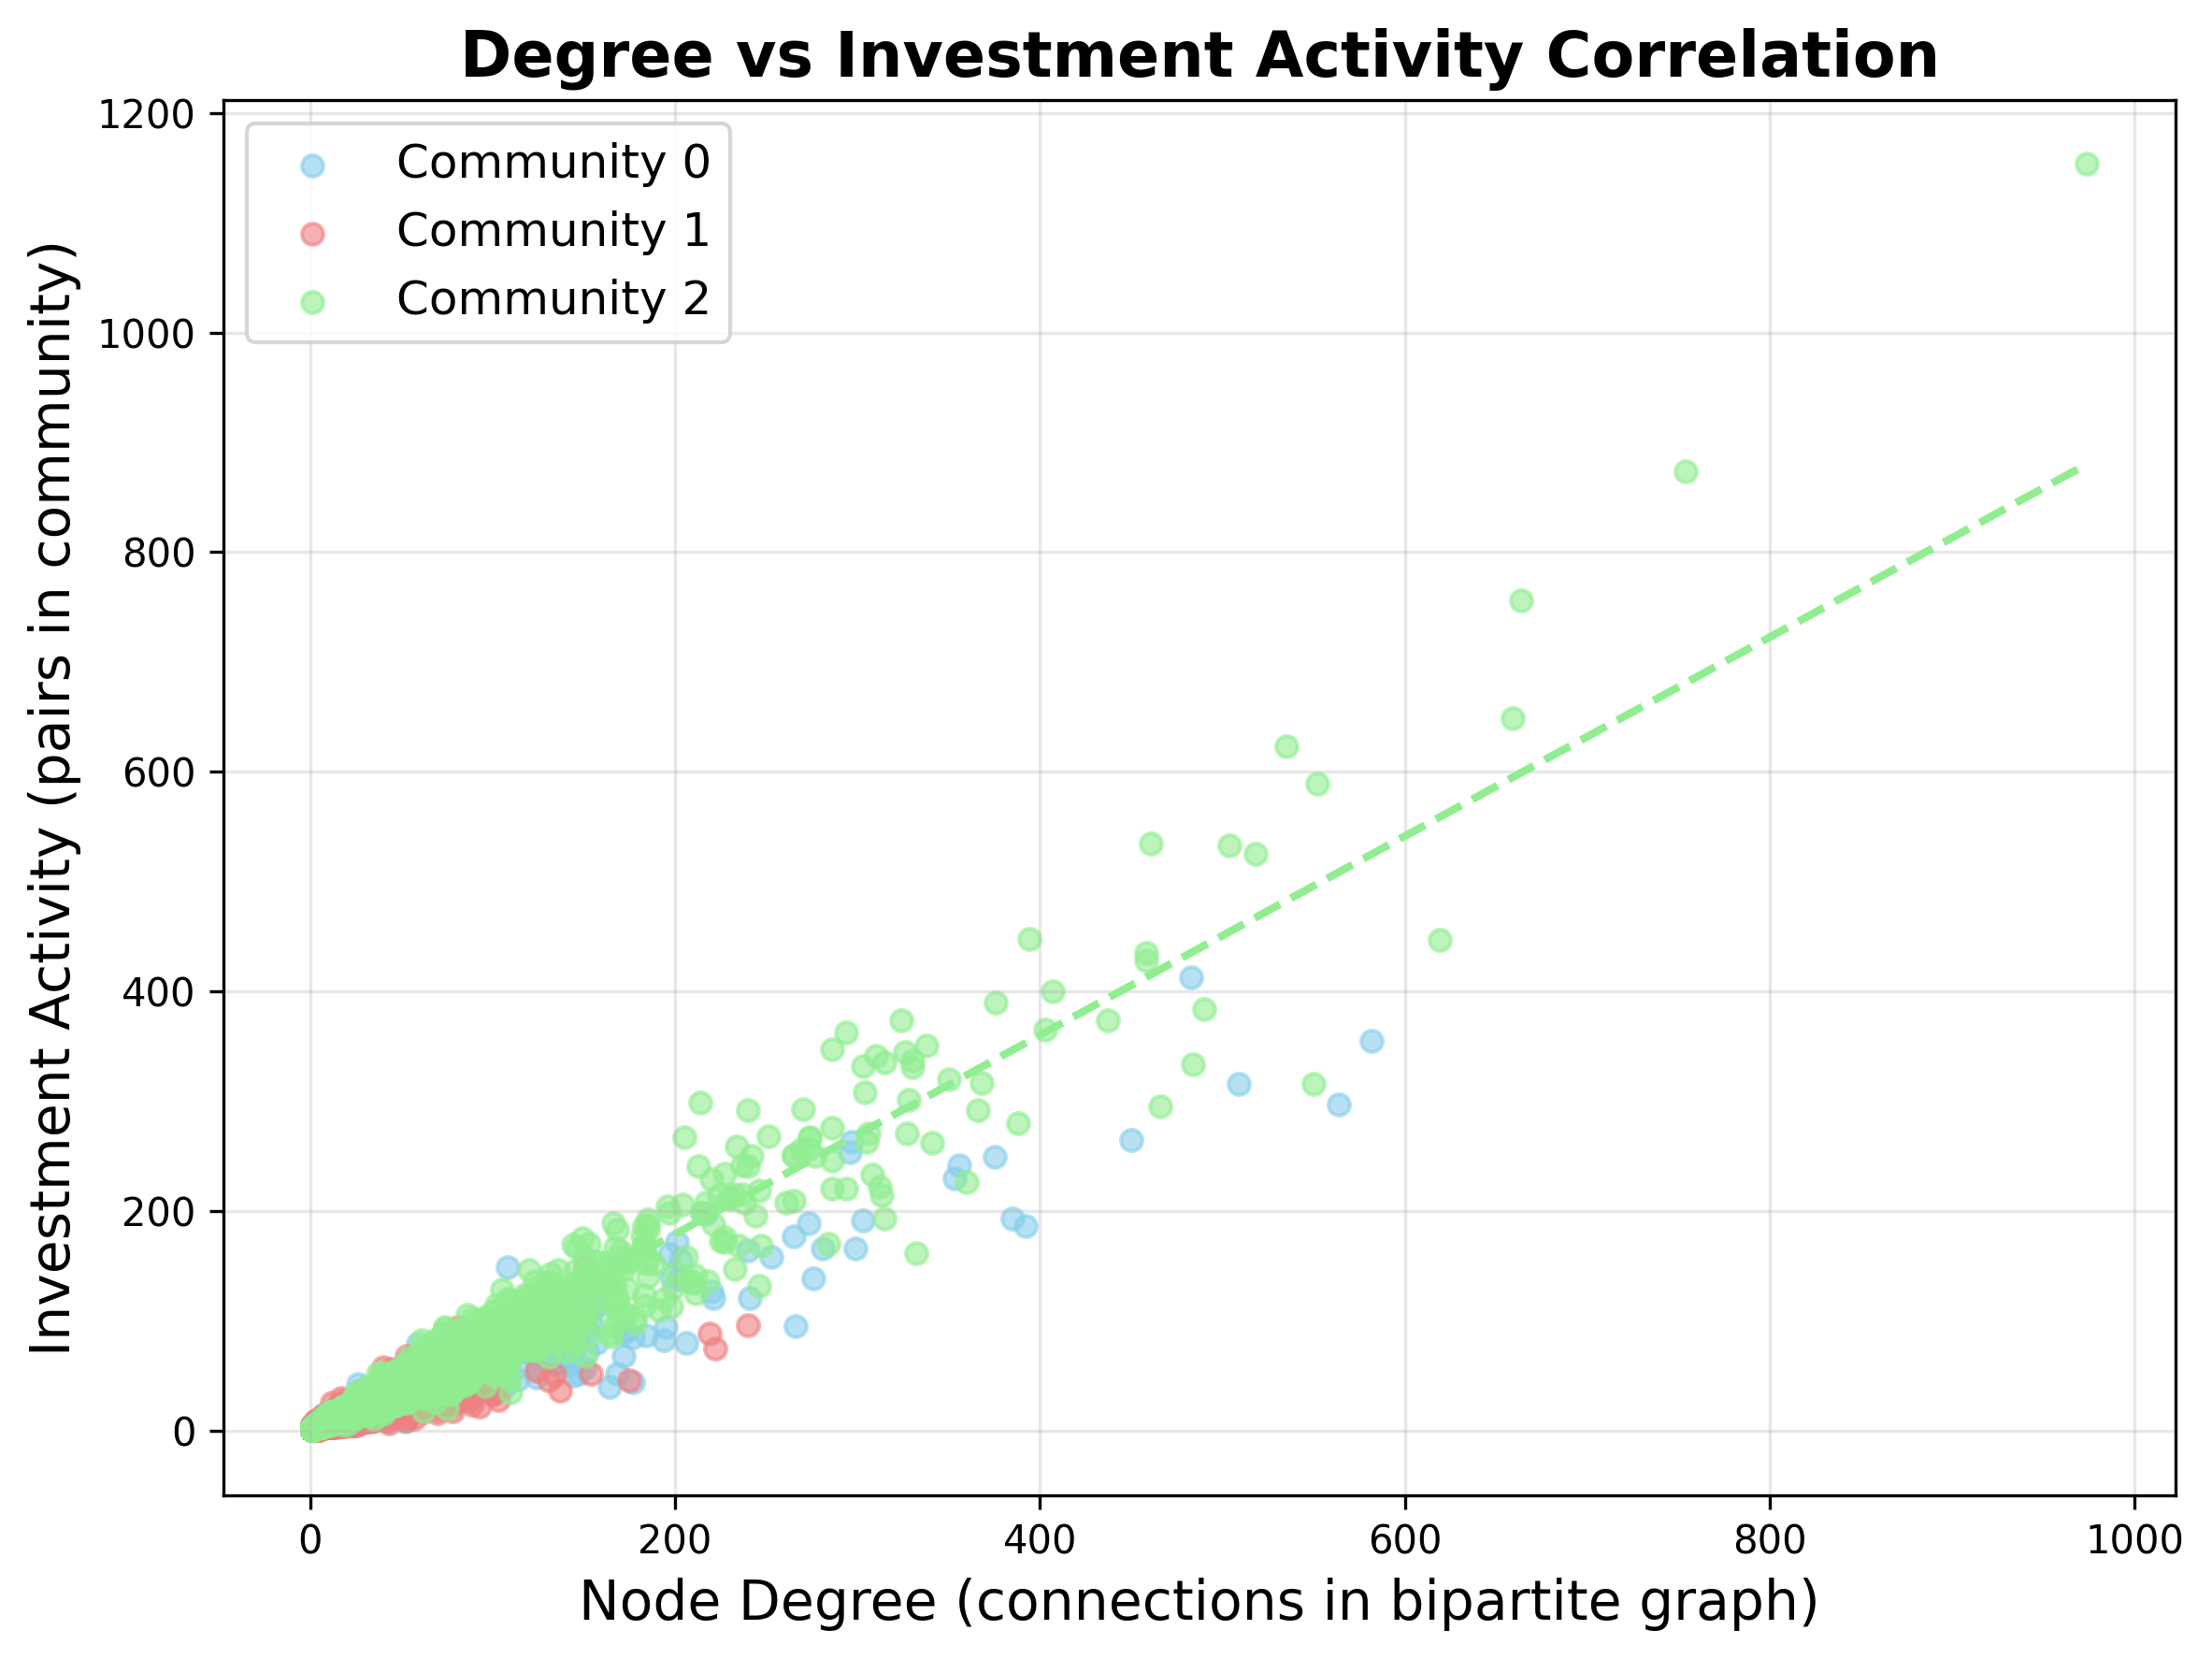
\includegraphics[width=1\textwidth]{../figures/us/degree_vs_investment_corr.png}
\caption{Relationship between node degree and investment activity for the three largest investor communities. The scatter plot demonstrates a positive correlation: higher-degree nodes tend to participate in more investment activities. This pattern is consistent across all communities, supporting the interpretation that network centrality is a strong predictor of investment frequency and influence within the venture capital ecosystem.}
\label{fig:degree_vs_activity}
\end{figure}

\subsubsection{Geographic Distribution}

Geographic analysis reveals distinct spatial clustering patterns across the three largest communities. Figure \ref{fig:geographic_distribution} illustrates the asymmetric geographic distributions between early-stage and late-stage investment networks.

\todo[inline]{Better format geographic distribution figure}

\begin{figure}[htp]
\centering
\begin{subfigure}{0.8\textwidth}
    \centering
    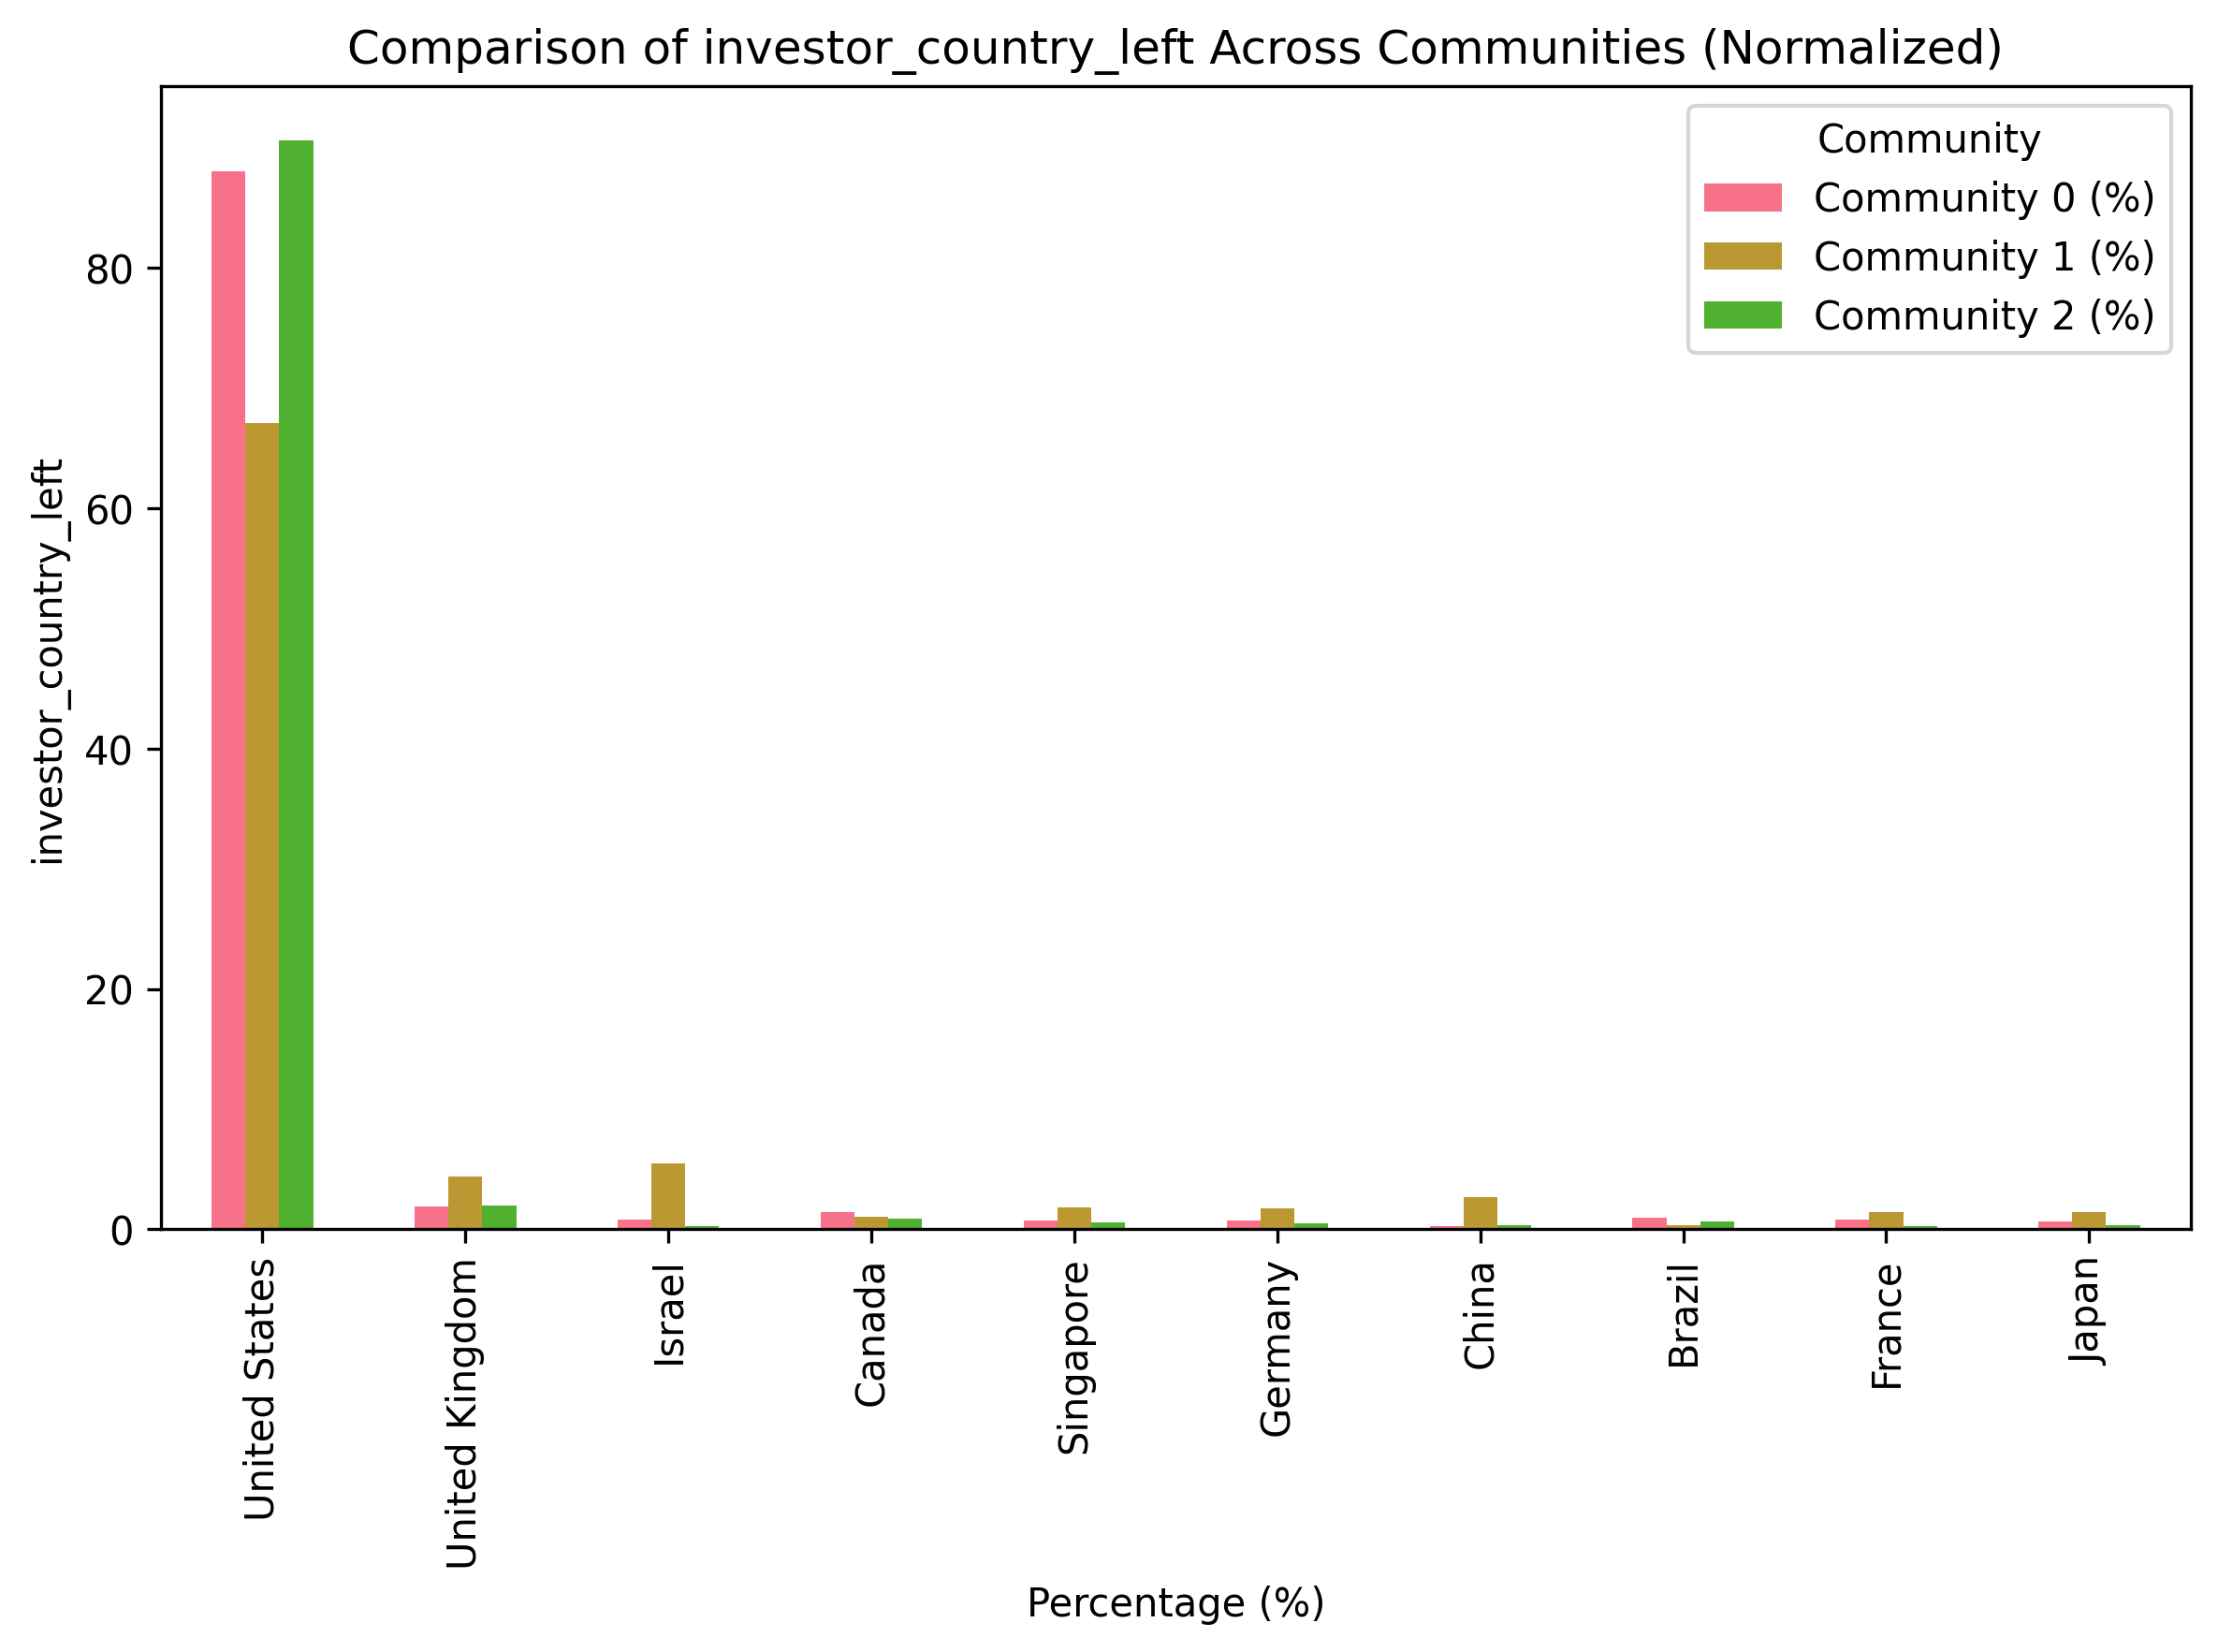
\includegraphics[width=1\textwidth]{../figures/us/categorical_comparison_investor_country_left.png}
    \caption{Late-stage investors geographic distribution (countries)}
    \label{fig:late_stage_geo}
\end{subfigure}

\vspace{0.5em}

\begin{subfigure}{0.8\textwidth}
    \centering
    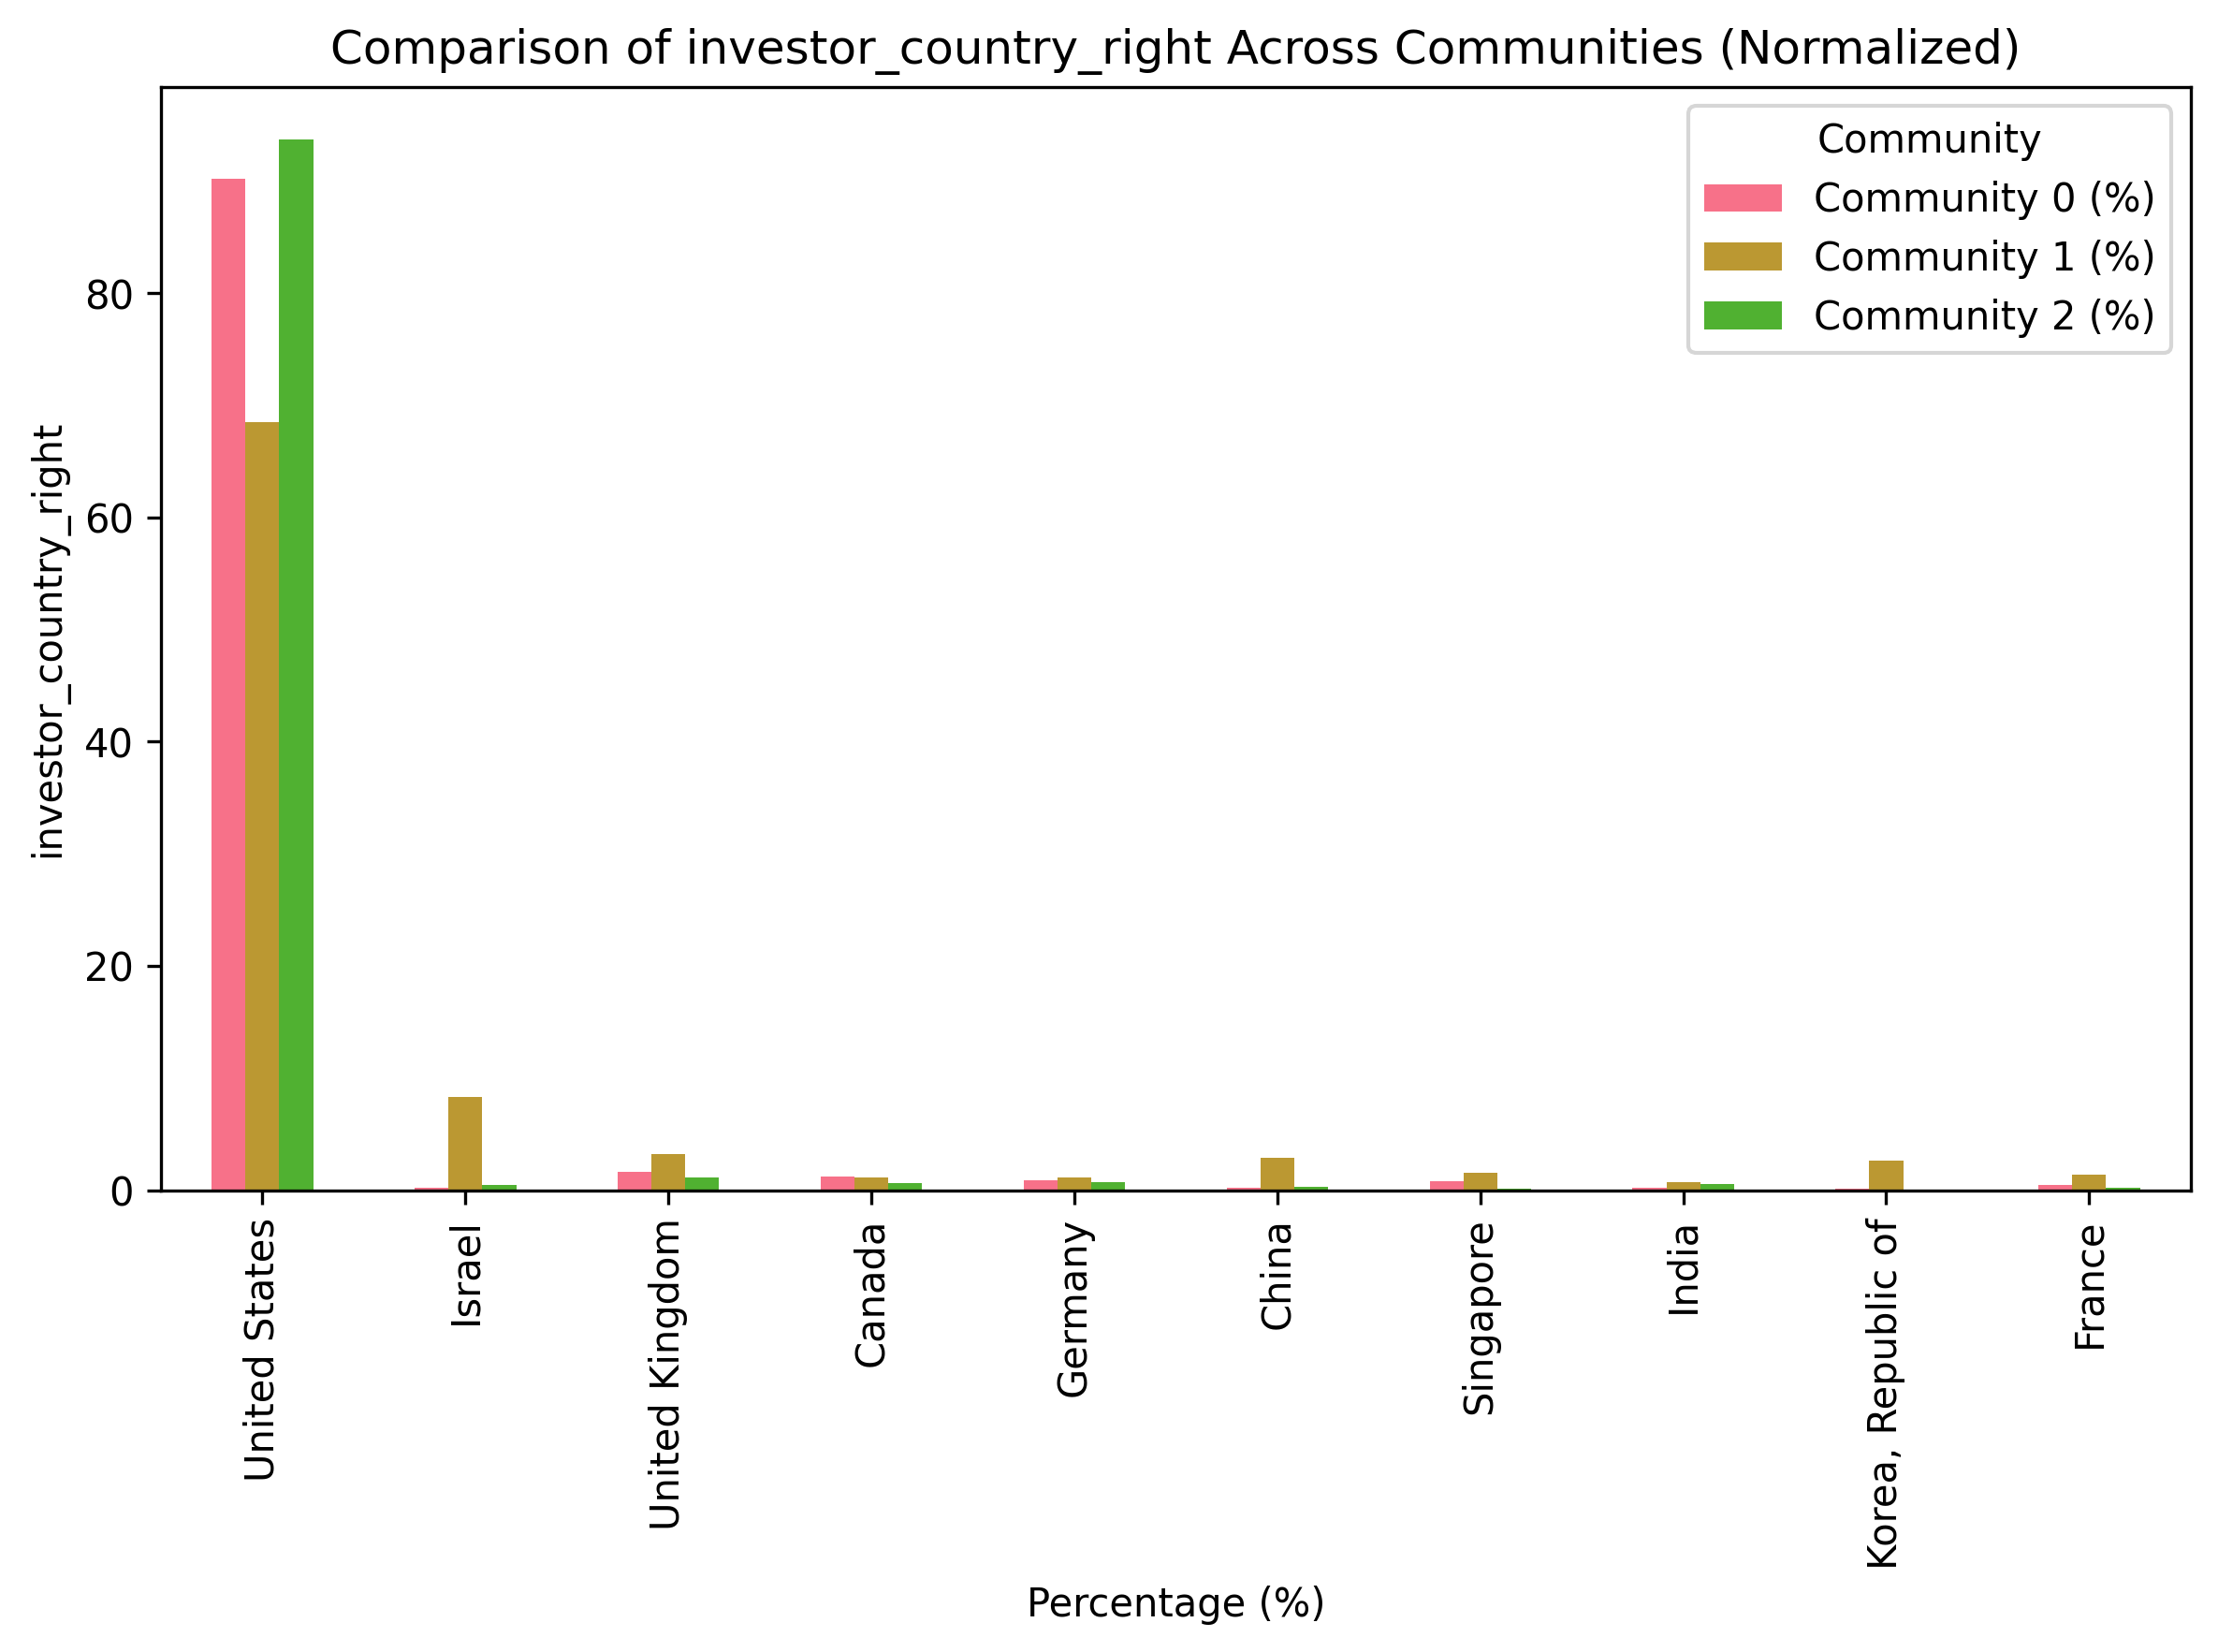
\includegraphics[width=1\textwidth]{../figures/us/categorical_comparison_investor_country_right.png}
    \caption{Early-stage investors geographic distribution (countries)}
    \label{fig:early_stage_geo}
\end{subfigure}
\caption{Geographic distribution of venture capital investors across the largest communities. The bipartite structure reveals differential geographic clustering between late-stage (top) and early-stage (bottom) investor networks, with Community 1 exhibiting greater international diversification compared to the U.S.-concentrated Communities 0 and 2.}
\label{fig:geographic_distribution}
\end{figure}

\begin{figure}[htp]
\centering
\begin{subfigure}{0.8\textwidth}
    \centering
    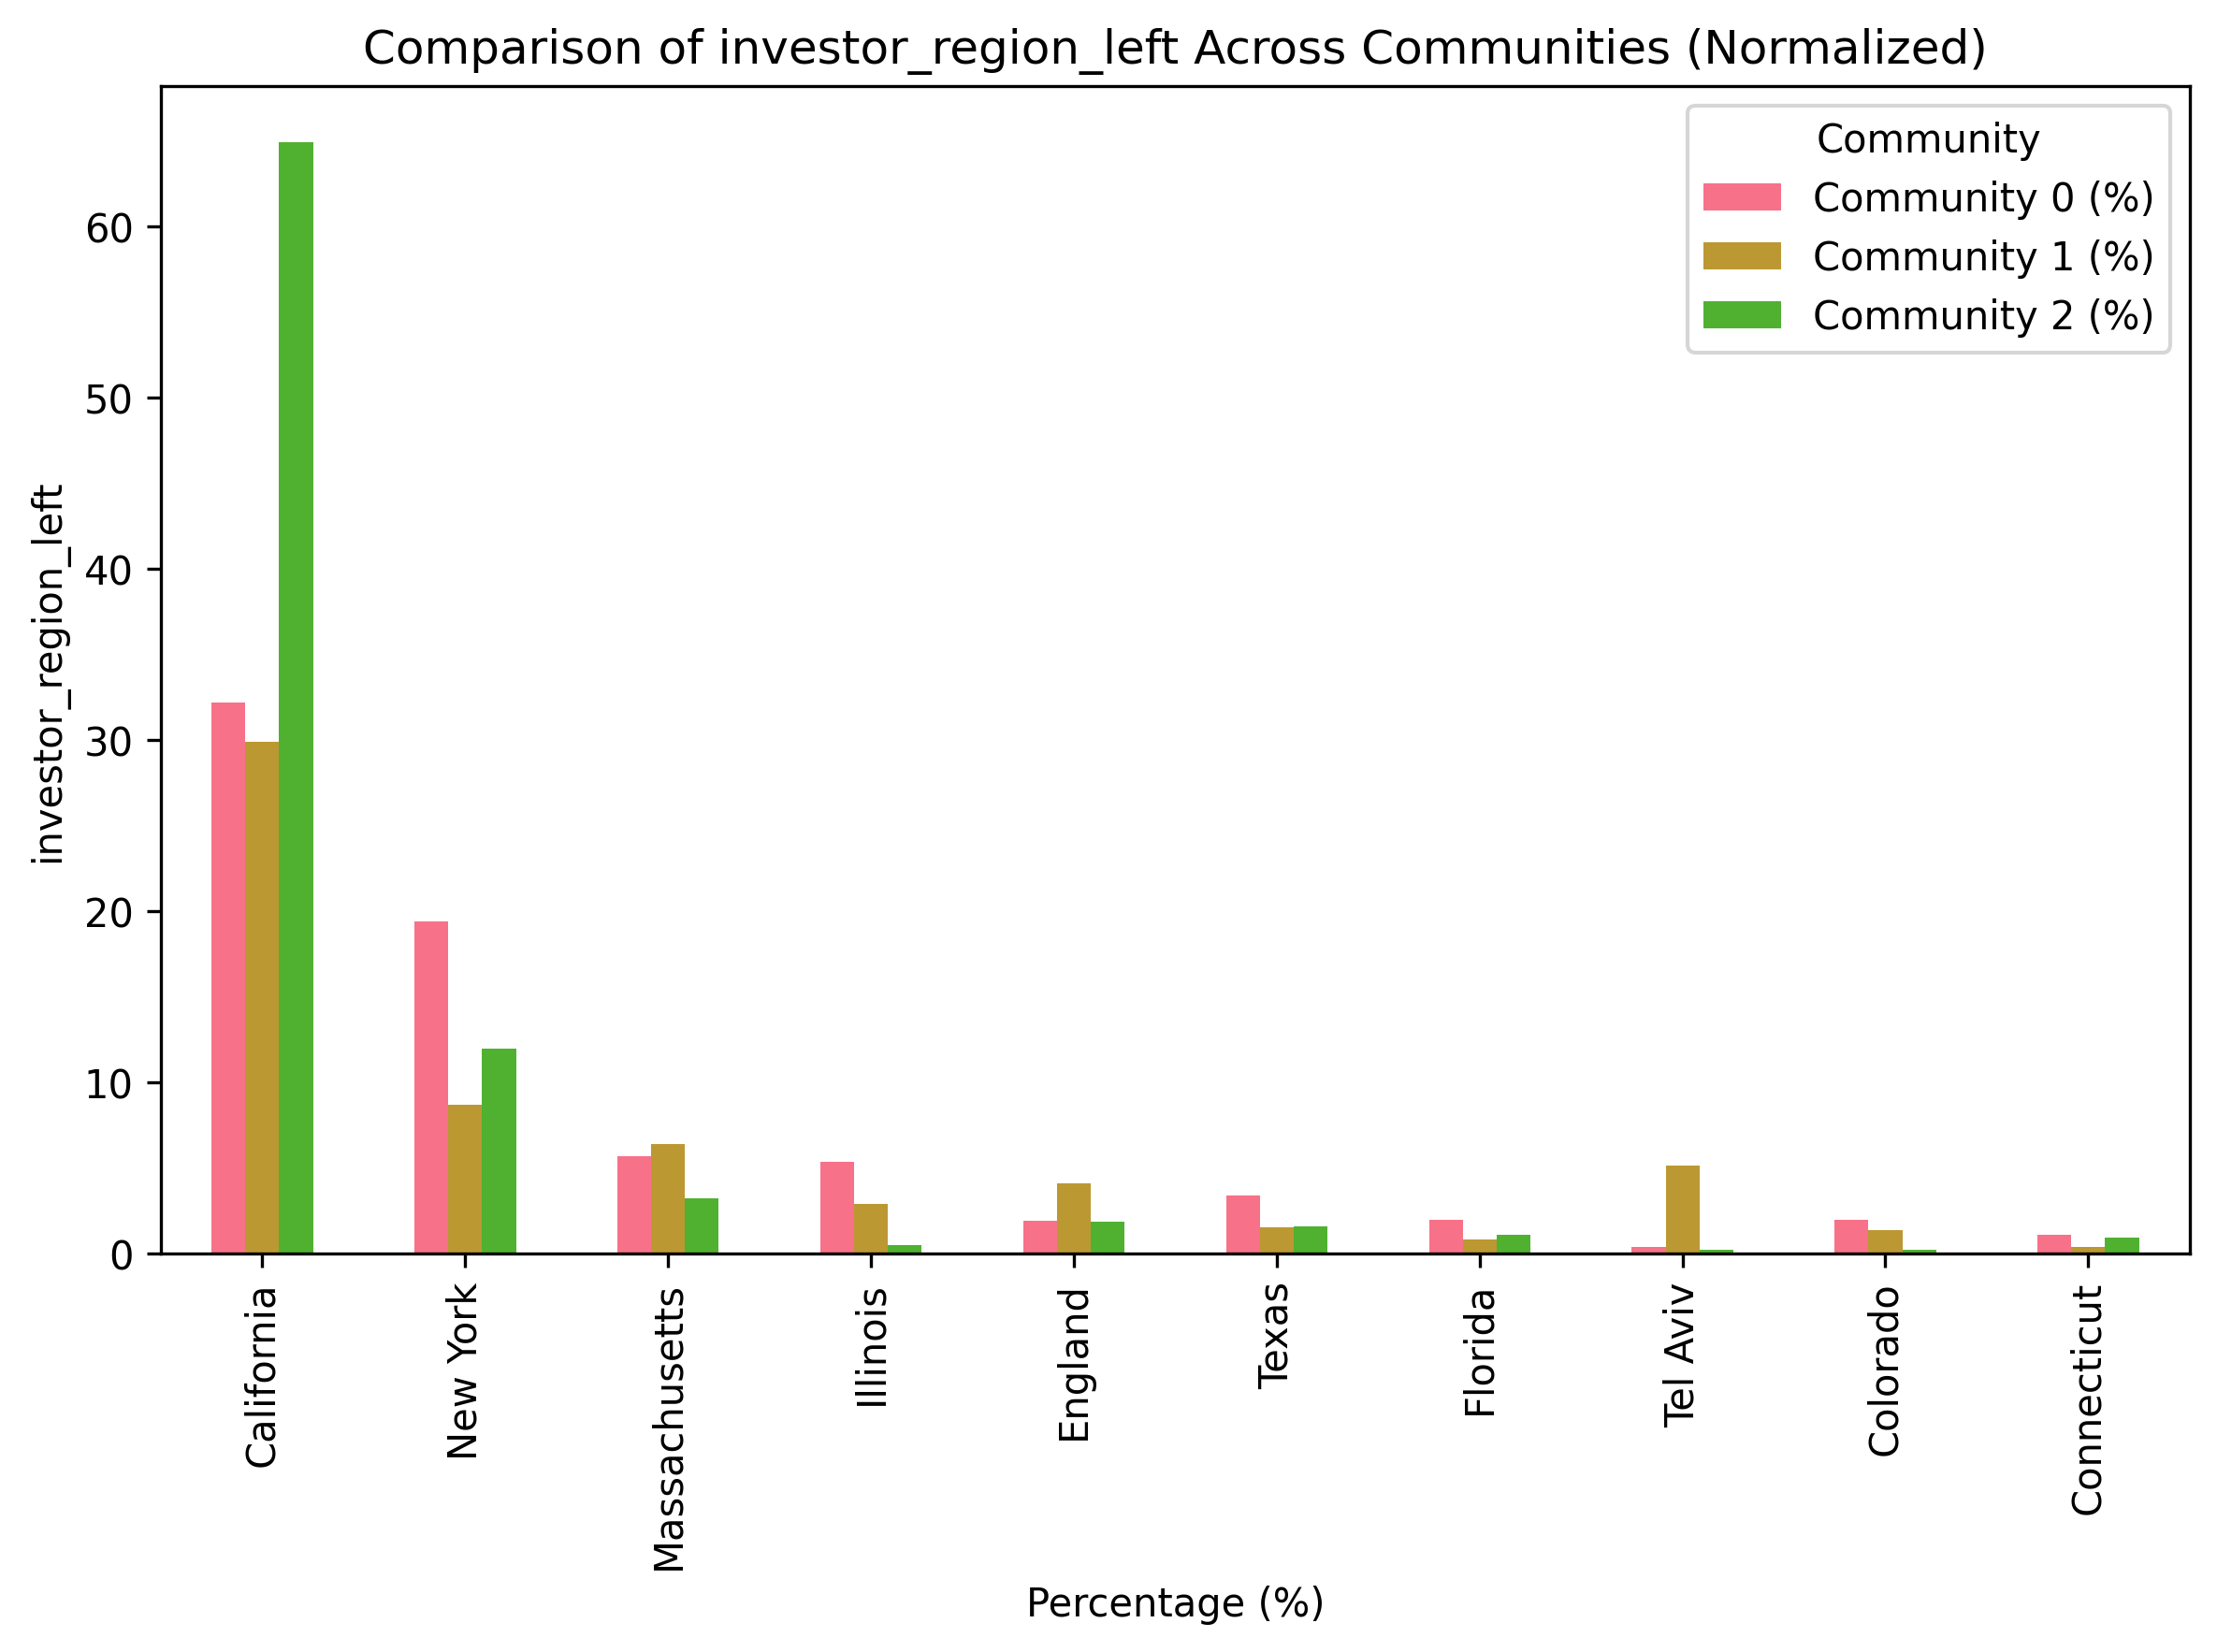
\includegraphics[width=1\textwidth]{../figures/us/categorical_comparison_investor_region_left.png}
    \caption{Late-stage investors geographic distribution (regions)}
    \label{fig:late_stage_geo}
\end{subfigure}

\vspace{0.5em}

\begin{subfigure}{0.8\textwidth}
    \centering
    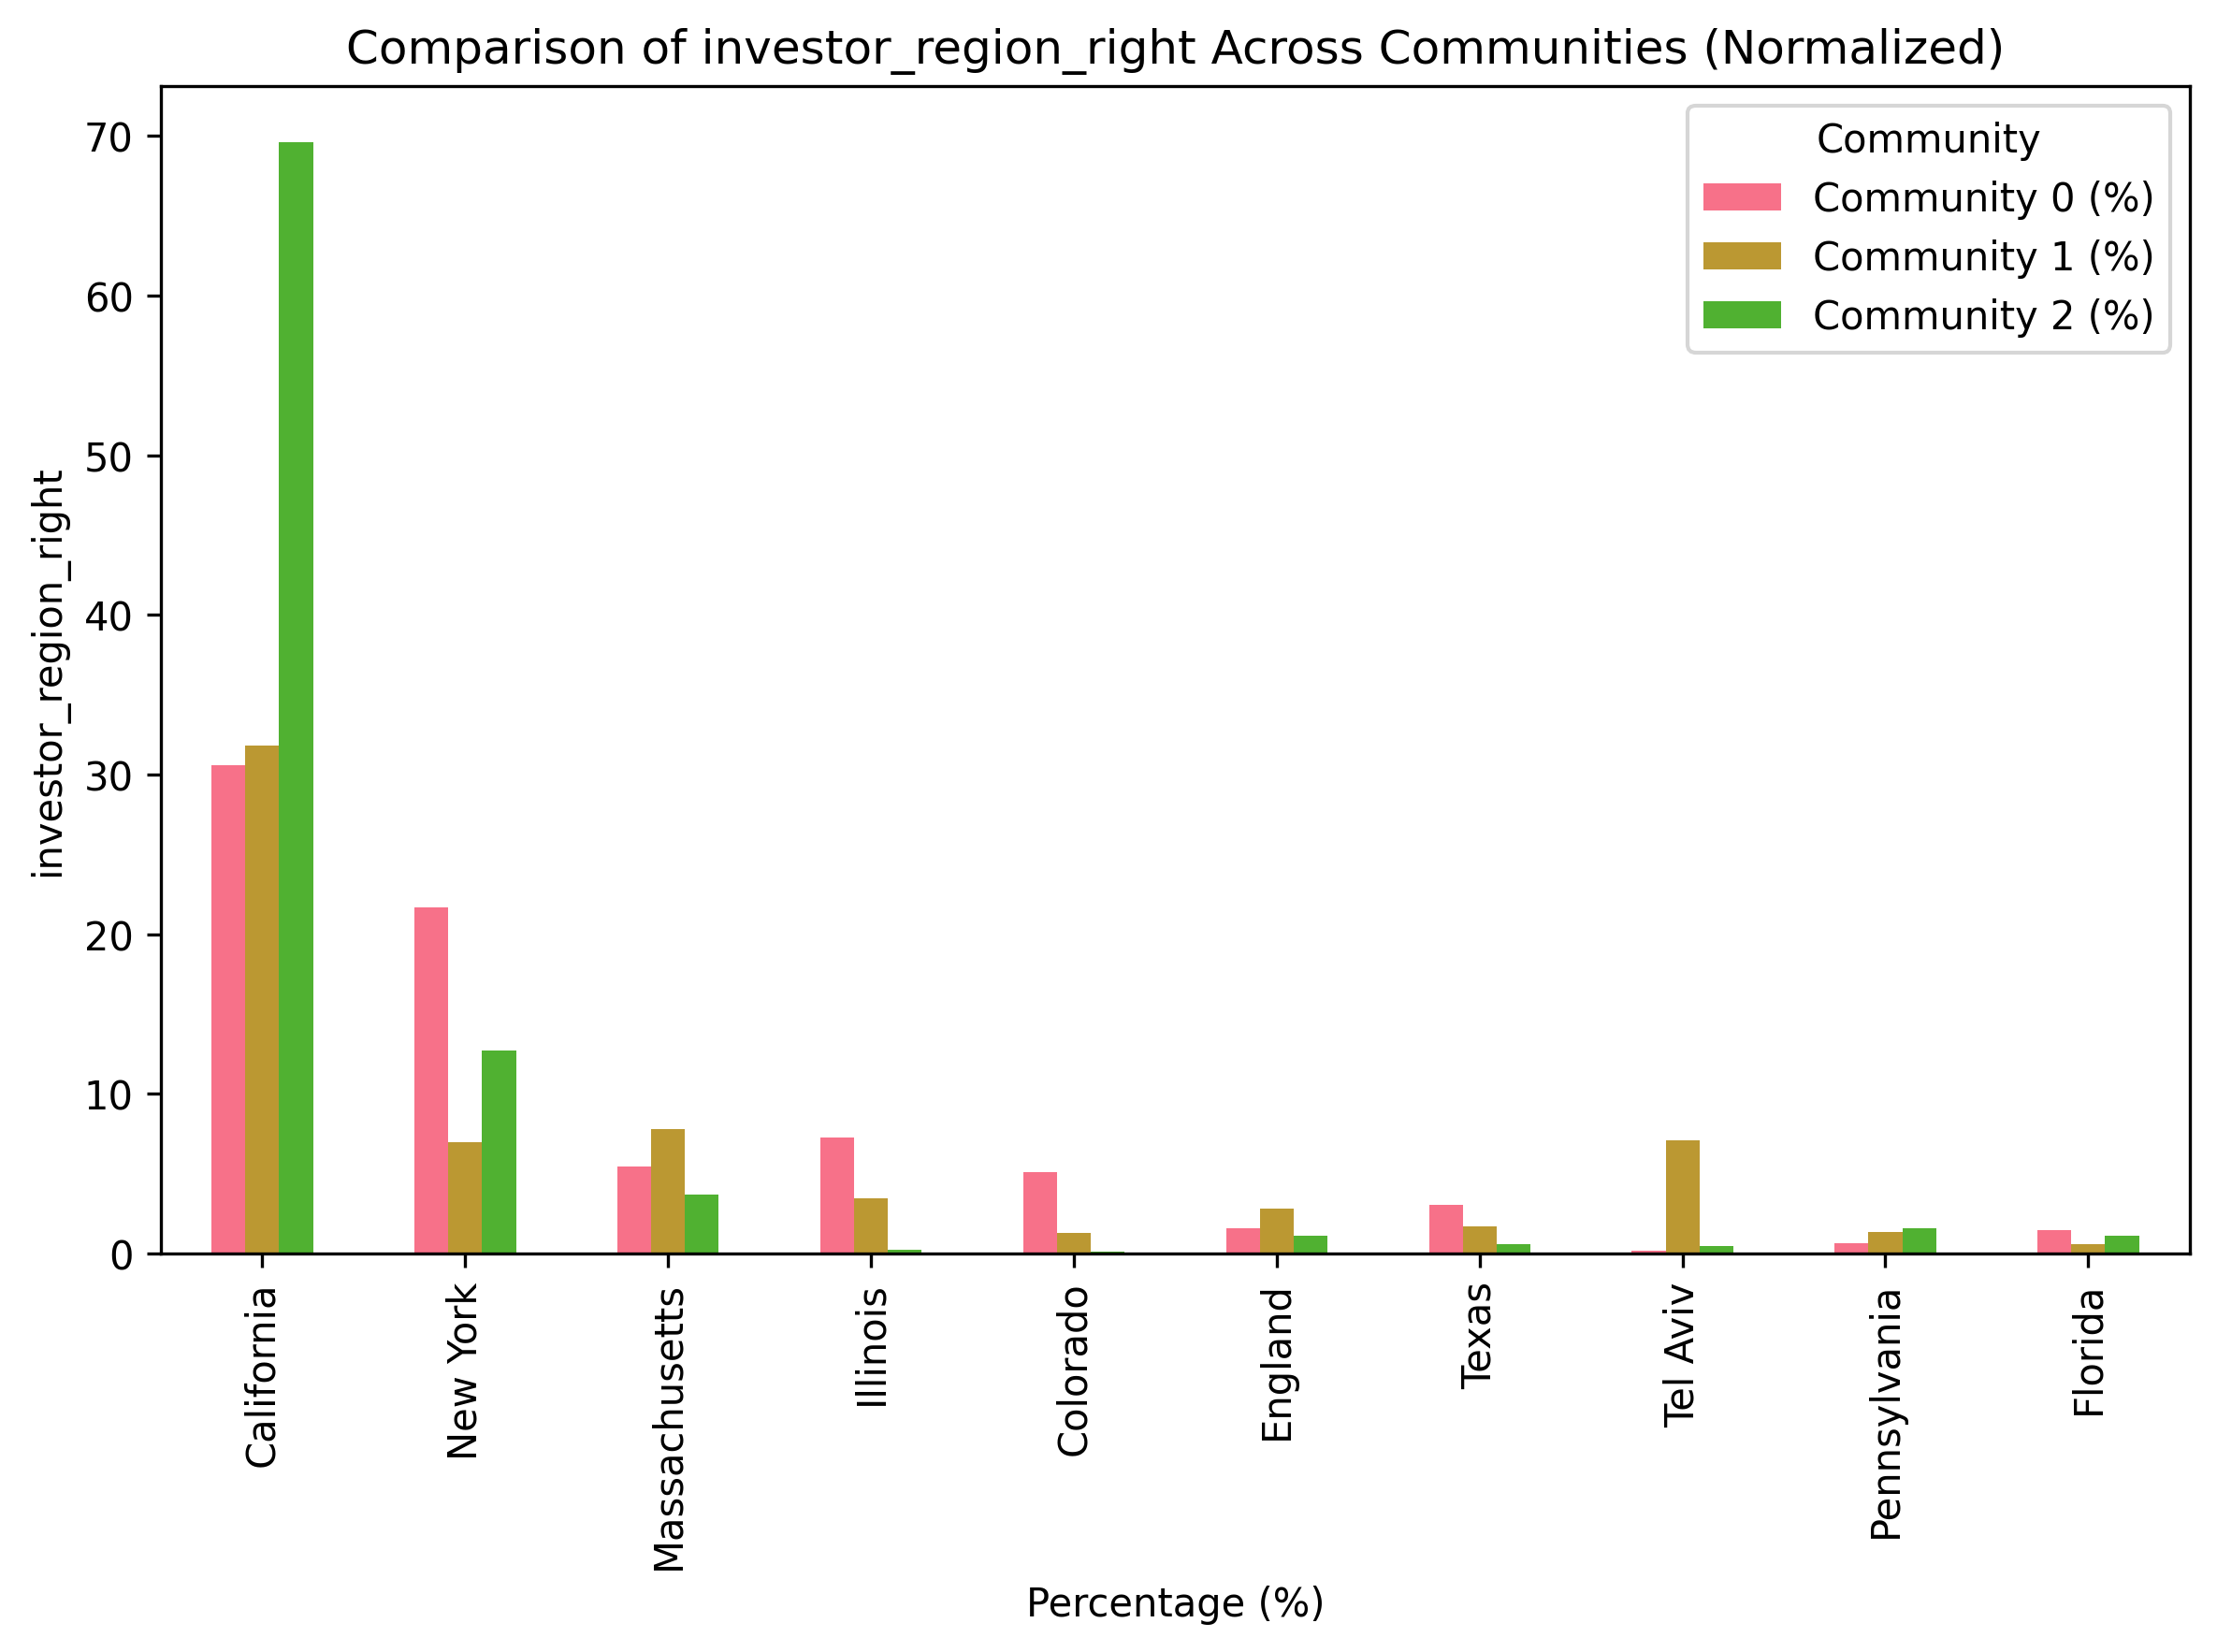
\includegraphics[width=1\textwidth]{../figures/us/categorical_comparison_investor_region_right.png}
    \caption{Early-stage investors geographic distribution (regions)}
    \label{fig:early_stage_geo}
\end{subfigure}
\caption{Geographic distribution of venture capital investors across regions}
\label{fig:geographic_distribution}
\end{figure}

% The geographic distributions exhibit notable asymmetries: late-stage investors demonstrate greater international representation, while early-stage investors show concentrated domestic clustering. This pattern suggests stage-specific geographic preferences that may reflect risk tolerance, regulatory constraints, or information asymmetries across international markets.

Communities 0 and 2 exhibit similar geographic profiles with predominantly American investors, reflecting the dominance of U.S.-based venture capital (important to remember our dataset contains only American startups' investments, which include international investors). 

However, regional analysis within the United States reveals a striking pattern: Community 2 demonstrates exceptional concentration in California, particularly Silicon Valley, with approximately 50\% more California-based investors than either Community 0 or Community 1 for both late-stage and early-stage investor categories.

This Silicon Valley concentration in Community 2 is particularly notable given the region's status as the world's premier innovation ecosystem. The dominance of California investors in this community, which also exhibits the highest transaction volumes, suggests potential advantages conferred by geographic clustering within innovation hubs.

% This pattern may reflect the dense information networks, frequent face-to-face interactions, and shared risk assessment practices characteristic of Silicon Valley's venture capital community.

In contrast, Community 1 demonstrates significantly greater international diversification, with substantial representation from Israel, the United Kingdom, China, South Korea, Singapore, and France. This international composition in Community 1 may reflect different risk tolerance profiles, regulatory environments, or access to cross-border deal flow compared to the more domestically concentrated communities.

\subsubsection{Funding Characteristics}

Analysis of funding patterns reveals that Community 2 exhibits substantially higher funding frequency and larger investment amounts compared to the other communities, as demonstrated in Figure \ref{fig:funding_characteristics}.

\todo[inline]{Add attachment with statistical proofs}

\begin{figure}[htbp]
\centering
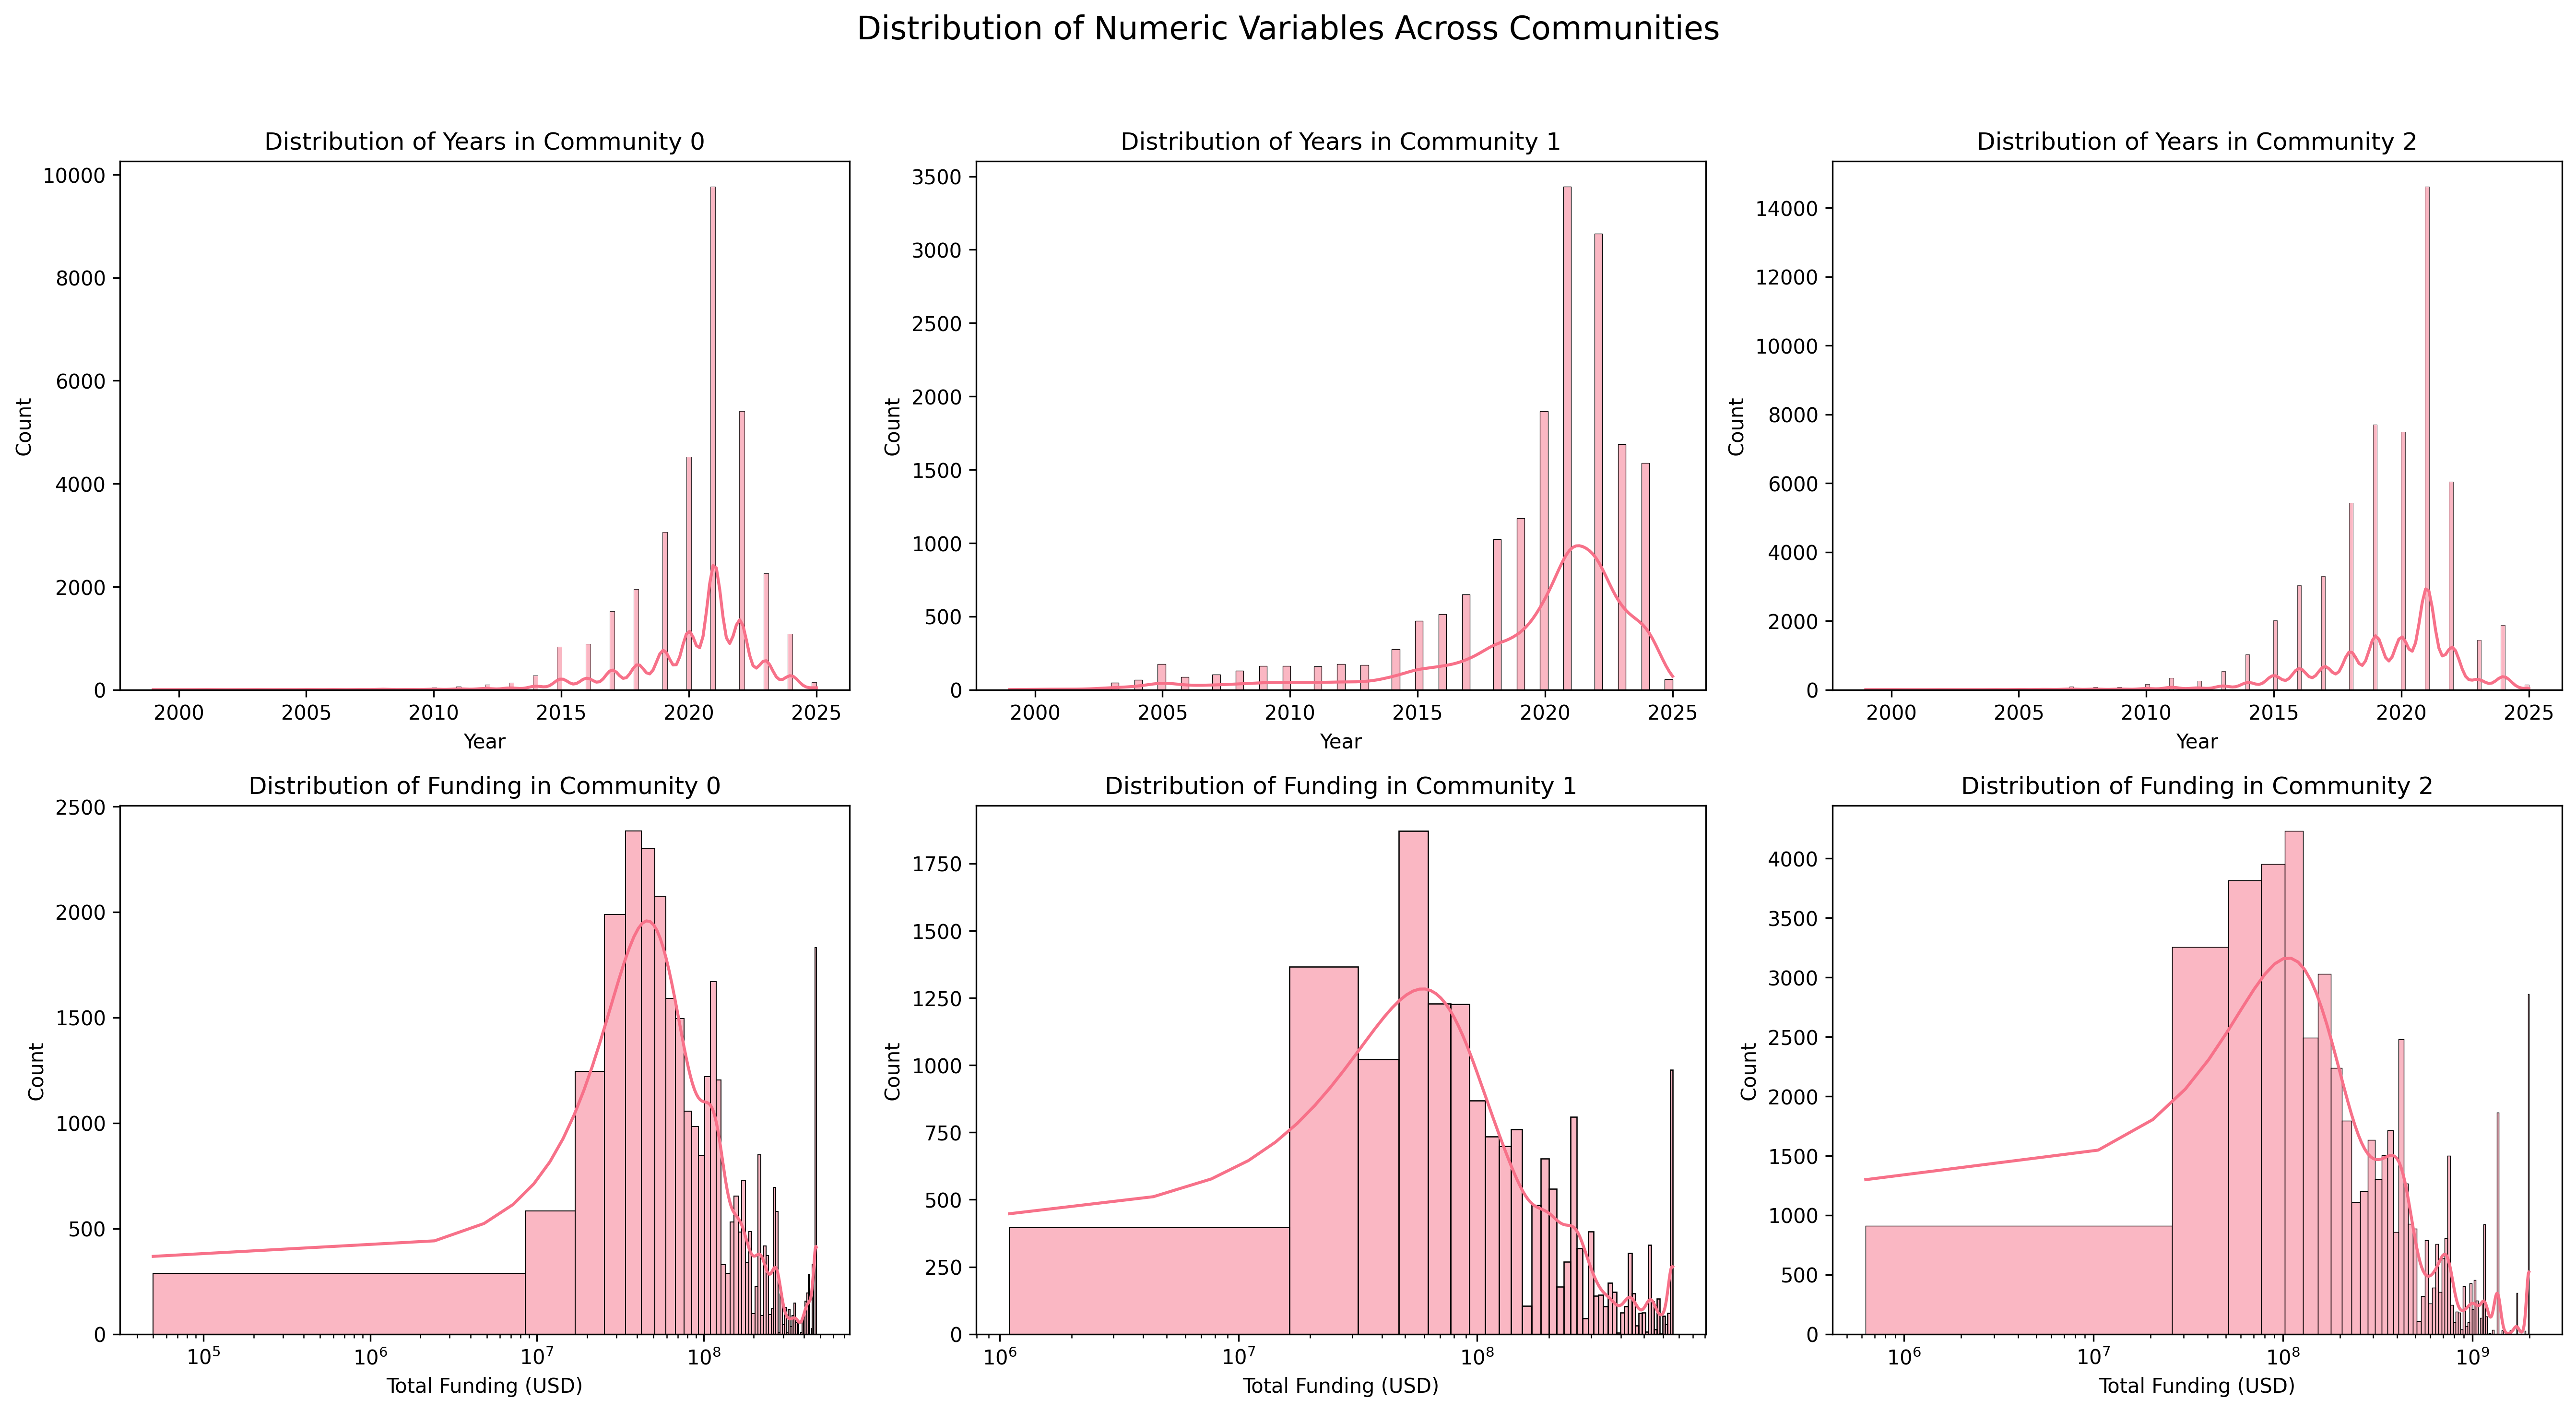
\includegraphics[width=1\textwidth]{../figures/us/numeric_variables_distribution.png}
\caption{Funding characteristics across the three largest investor communities. The analysis reveals systematic differences in investment amounts, round frequency, and funding patterns between communities, with different organizational structures exhibiting distinct capital deployment strategies.}
\label{fig:funding_characteristics}
\end{figure}

\todo[inline]{plot a graph of distribtuion of invesments among degrees of investors}

Furthermore, communities exhibit concentrated capital deployment patterns, with higher-degree investors participating in larger funding rounds while maintaining broader portfolio diversification. This suggests that certain organizational structures may create more efficient capital allocation mechanisms compared to other network configurations.

Despite superficial similarities between Communities 0 and 2 in terms of size and geographic concentration within the United States, Community 2 appears to confer distinctive advantages in organizational efficiency. While both communities share comparable scales and American investor bases, Community 2's organizational structure enables it to achieve substantially higher transaction volumes (33.6\% vs. 19.4\% of total investments) and more comprehensive funding coverage across all investment stages. 

This pattern suggests that specific network topologies, rather than community size or geographic distribution alone, may be critical determinants of investment ecosystem efficiency.

\todo[inline]{add literature base for this strong assumption}

\subsubsection{Investment Stage Preferences}

The investment stage distributions reveal systematic specialization patterns across communities that align with their geographic profiles and transaction volumes. Figure \ref{fig:investment_stage_distribution} demonstrates the distribution patterns of investment types within the bipartite network structure.

\begin{figure}[htbp]
\centering
\begin{subfigure}[t]{0.48\textwidth}
    \centering
    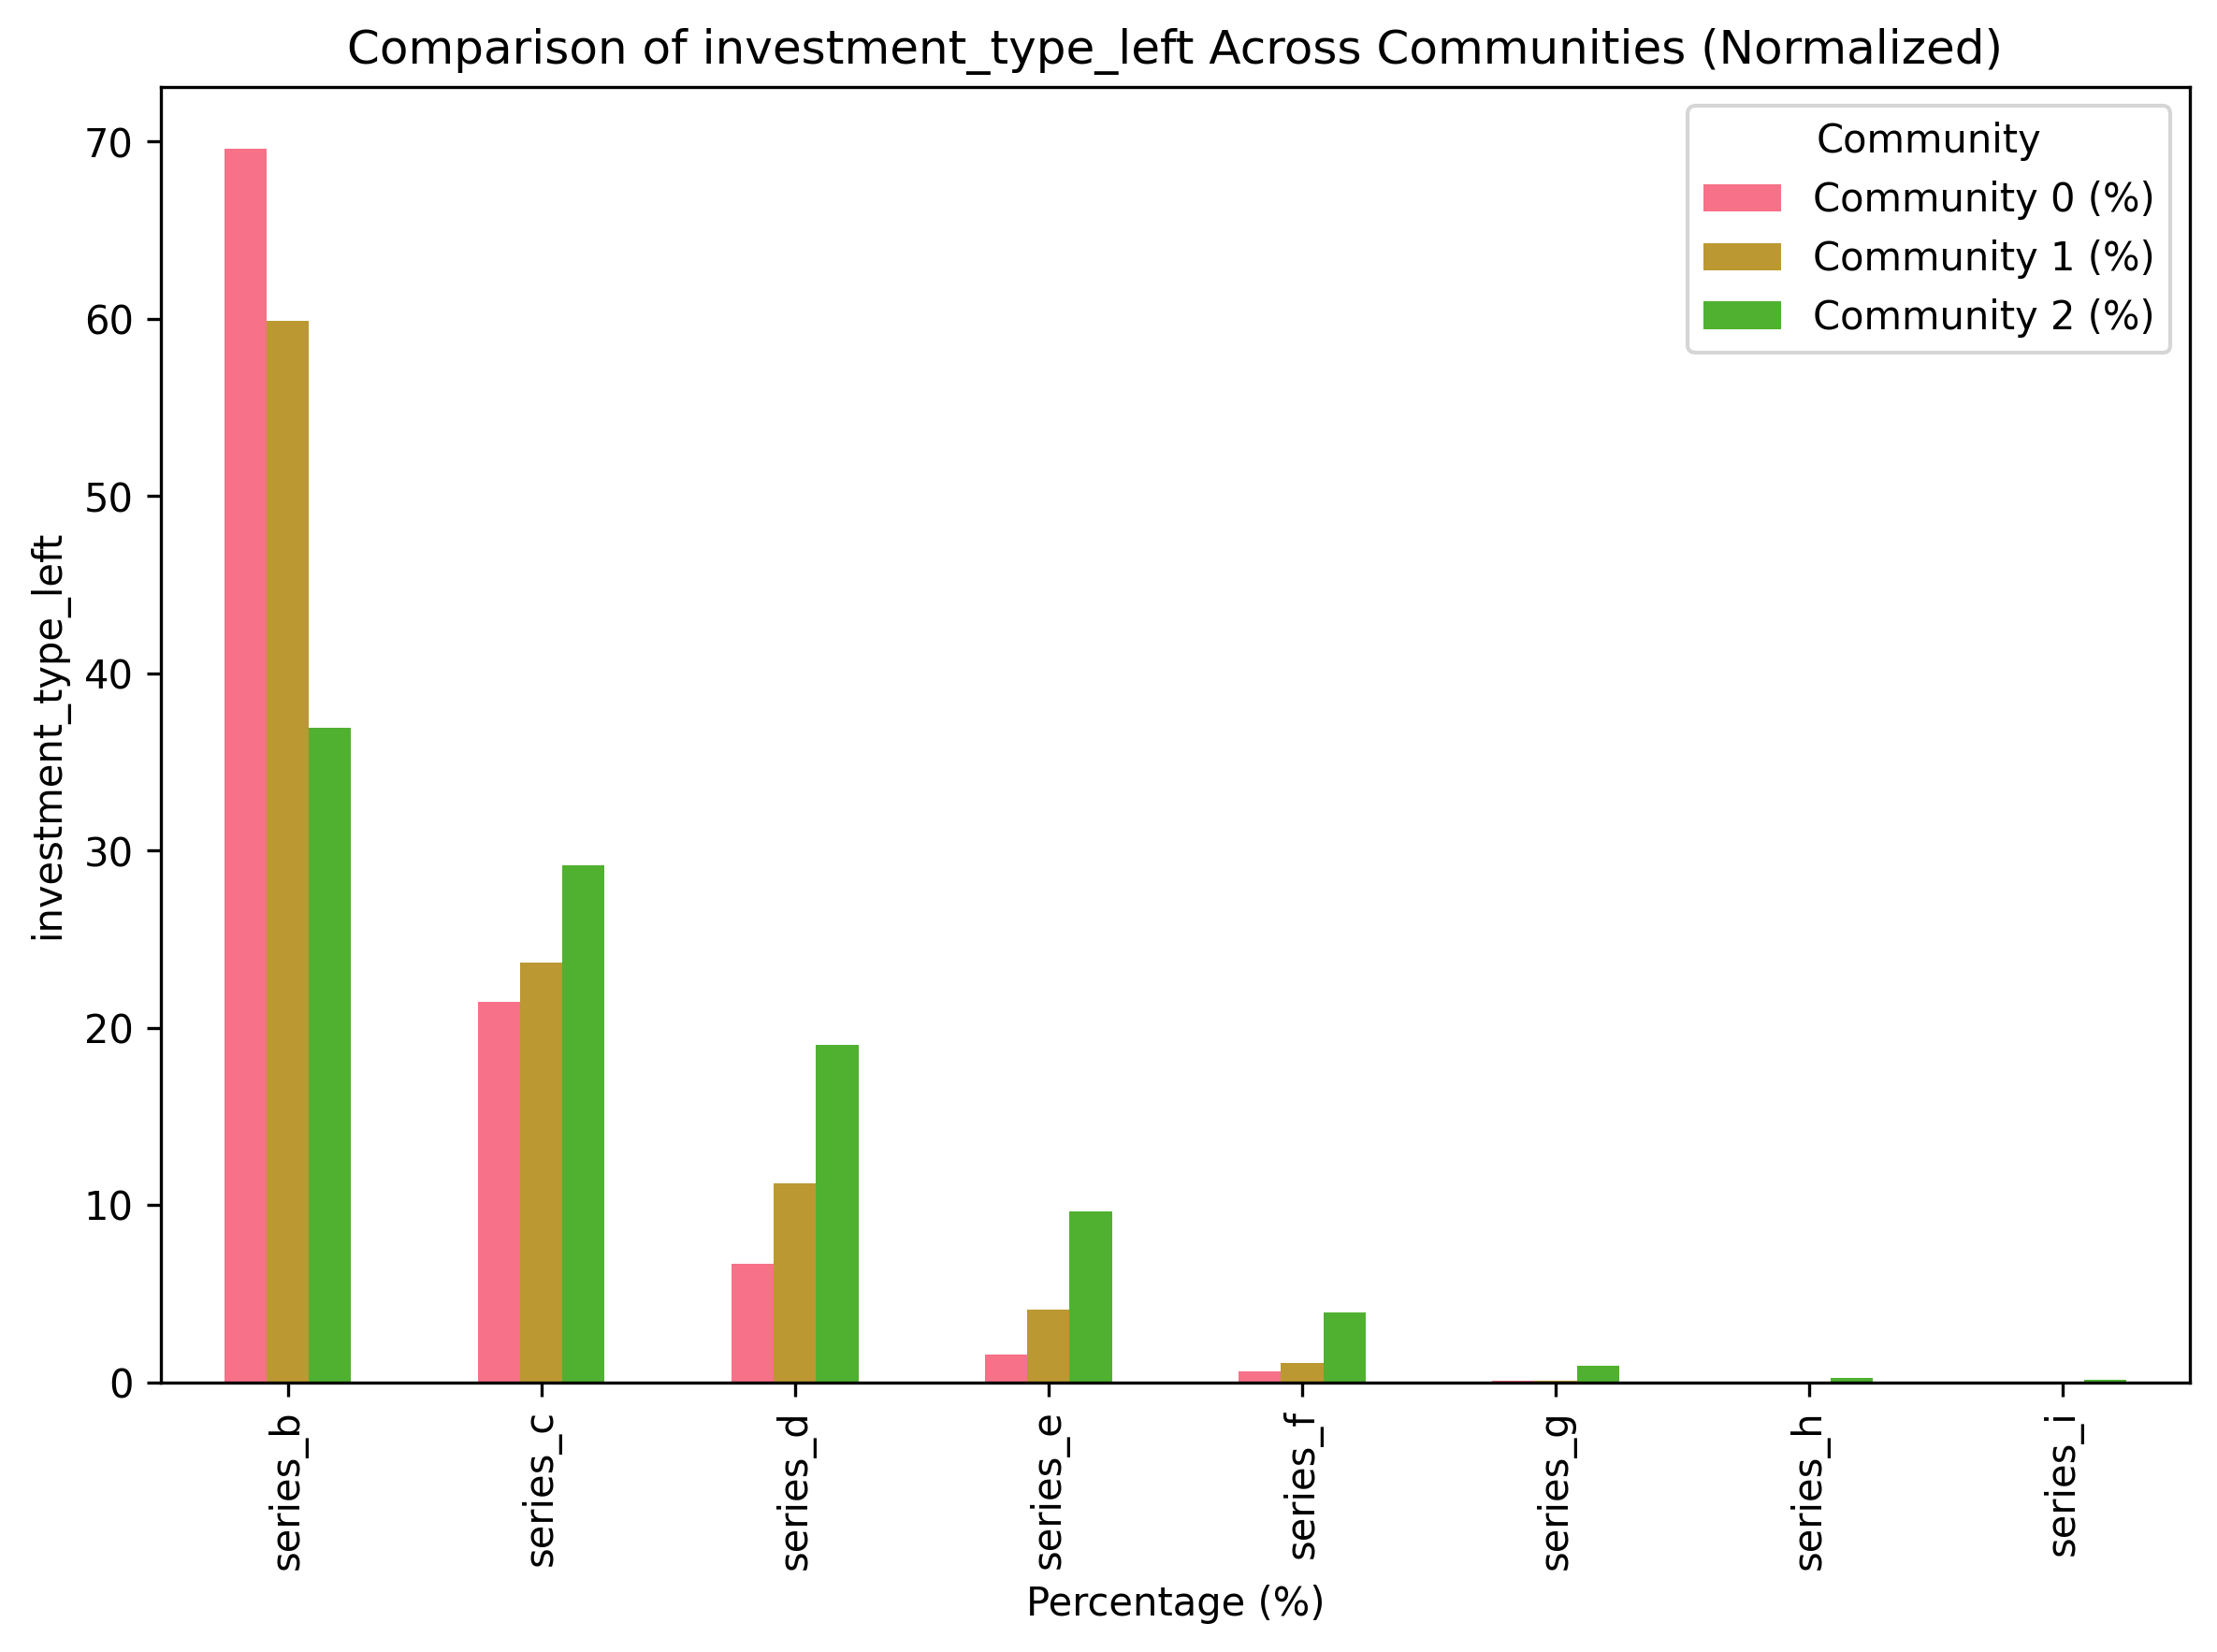
\includegraphics[width=\textwidth]{../figures/us/categorical_comparison_investment_type_left.png}
    \caption{Late-stage investment types distribution}
    \label{fig:late_stage_types}
\end{subfigure}
\hfill
\begin{subfigure}[t]{0.48\textwidth}
    \centering
    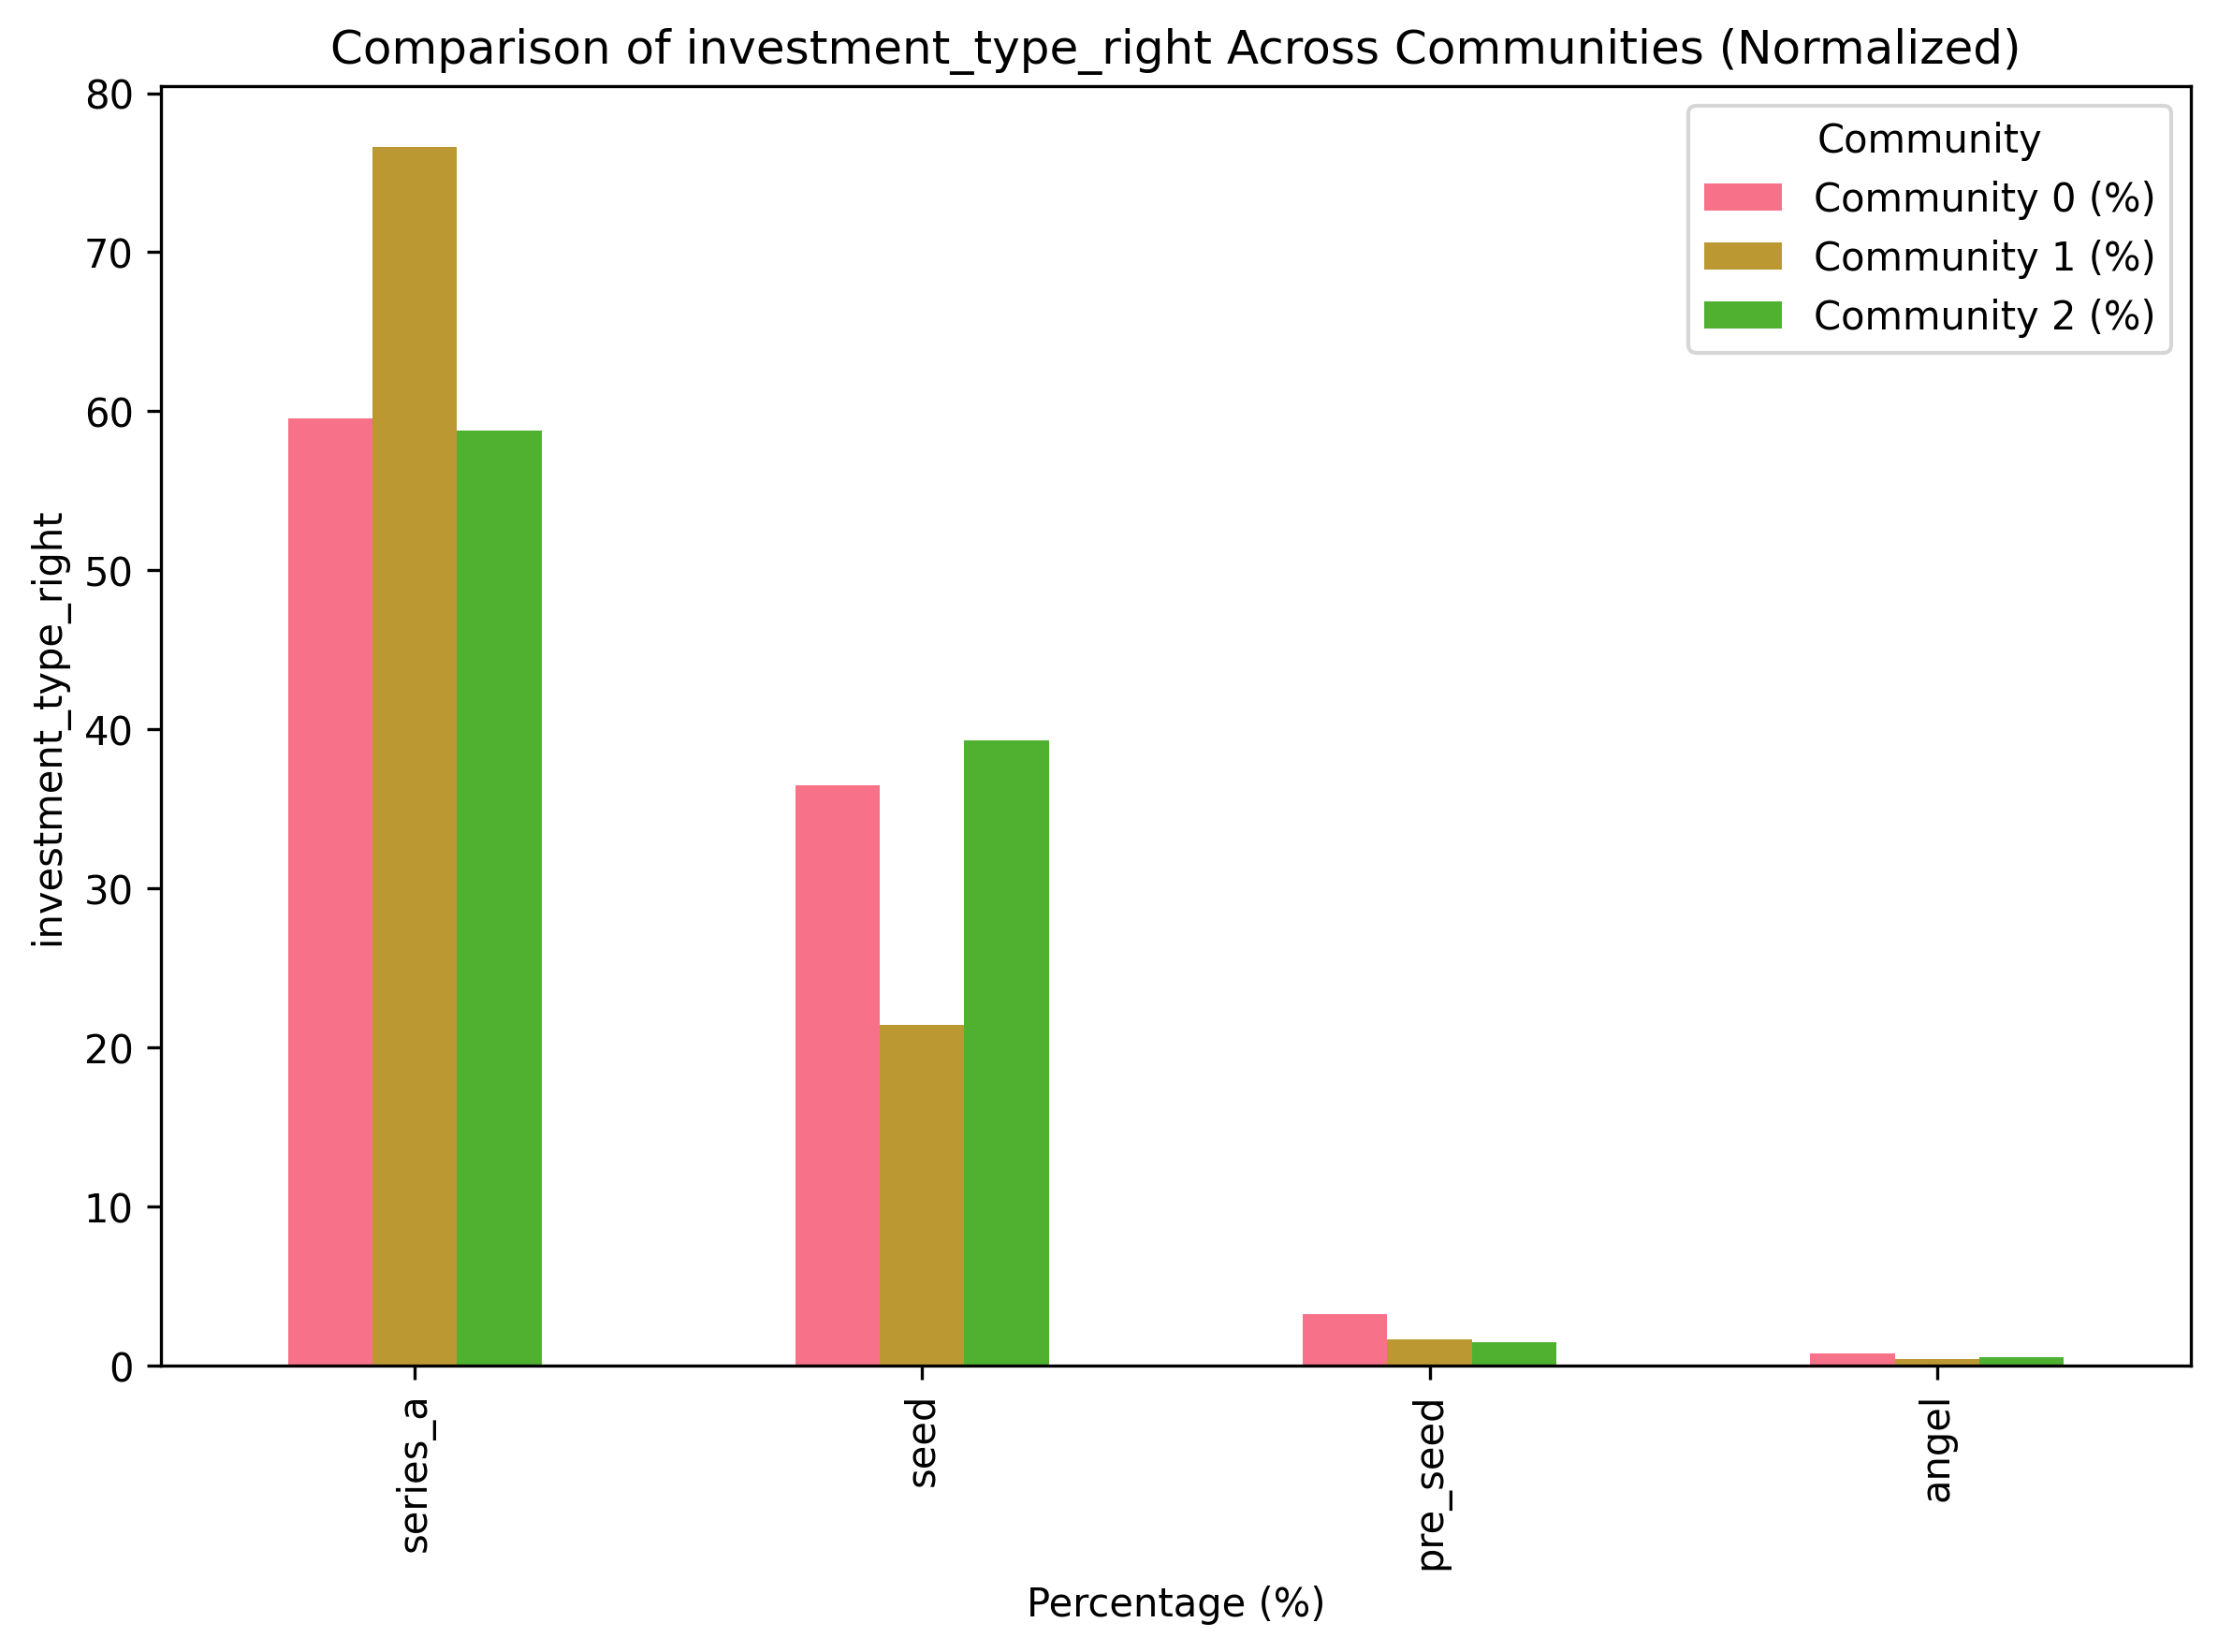
\includegraphics[width=\textwidth]{../figures/us/categorical_comparison_investment_type_right.png}
    \caption{Early-stage investment types distribution}
    \label{fig:early_stage_types}
\end{subfigure}
\caption{Investment stage distribution across the three largest communities. The distribution patterns reveal stage-specific specialization within investor communities.}
\label{fig:investment_stage_distribution}
\end{figure}

\textbf{Late-stage investment patterns:} Community 2 dominates Series C and later funding rounds, demonstrating its role in growth-stage capital deployment. Community 1, despite its smaller transaction volume, shows strong representation in Series B and later stages, with participation rates exceeding Community 0 in Series C and beyond. Community 0 exhibits particular strength in Series B rounds while maintaining lower participation in later stages compared to Community 2.

\textbf{Early-stage investment patterns:} Community 2 shows prominence in seed-stage investments while maintaining comparable levels to Community 0 in Series A funding. Both Communities 0 and 2 participate actively in angel and seed rounds, though Community 0 shows relatively higher pre-seed activity. Community 1 demonstrates concentrated focus on Series A investments, aligning with its international profile and suggesting specialization in cross-border early-growth funding.

These stage-specific patterns suggest that Community 2's organizational structure facilitates participation across the entire funding spectrum, from seed to late-stage rounds, potentially enabling more comprehensive support for portfolio companies throughout their development lifecycle.

\subsubsection{Sectoral Focus}

The sectoral analysis reveals distinct specialization patterns that align with each community's structural and geographic characteristics. Figure \ref{fig:sectoral_distribution} illustrates the distribution of investment focus across technology sectors, demonstrating how different communities exhibit varying degrees of sectoral concentration.

\begin{figure}[htbp]
\centering
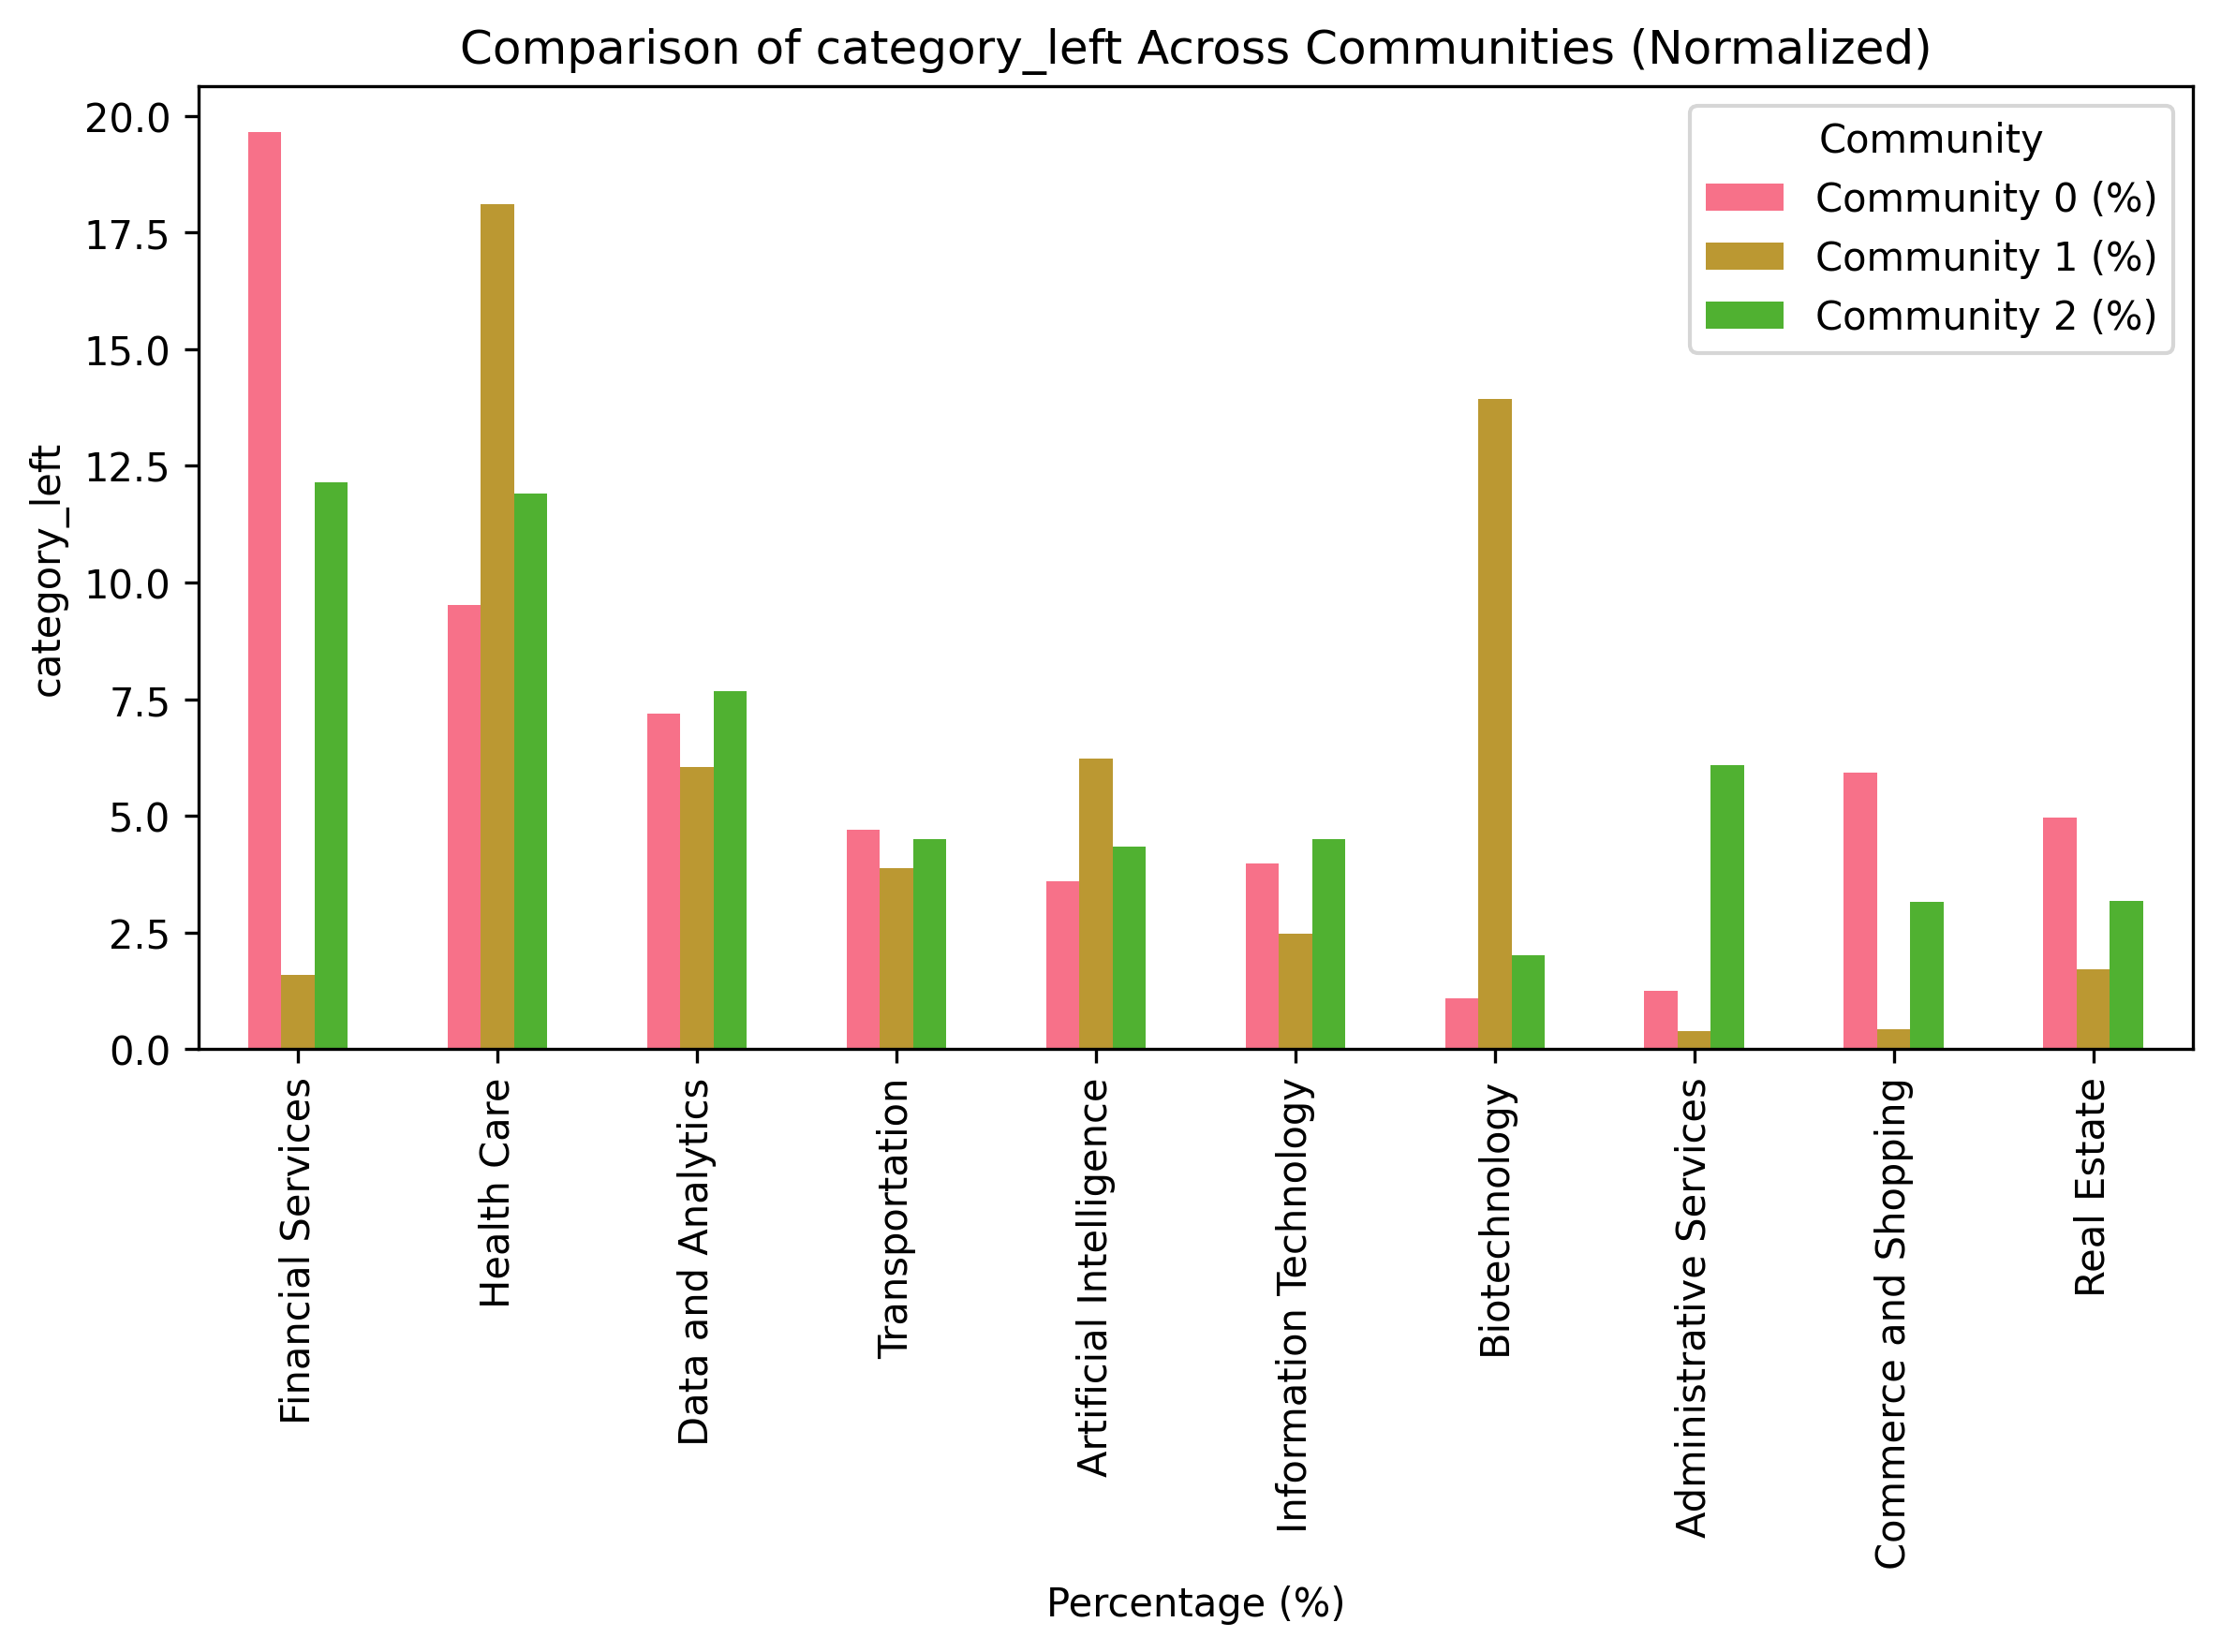
\includegraphics[width=1\textwidth]{../figures/us/categorical_comparison_category_left.png}
\caption{Sectoral distribution across the three largest investor communities. The analysis reveals differential industry focus patterns, with certain communities demonstrating concentrated investment strategies in specific technology sectors while others maintain broader sectoral diversification.}
\label{fig:sectoral_distribution}
\end{figure}

\todo[inline]{Comment sectorial distribution}

\textbf{Community 0:} Concentrates in real estate, commerce and shopping, and financial services, while maintaining standard representation in information technology and artificial intelligence. Notably absent from administrative services and biotechnology, suggesting specialized expertise in consumer-facing and financial technology sectors.

\textbf{Community 1:} Specializes significantly in biotechnology and healthcare, with enhanced artificial intelligence focus compared to other communities. Shows reduced interest in real estate, commerce and shopping, and administrative services. The biotechnology concentration aligns with its international composition, potentially reflecting access to global biotech innovation hubs.

\textbf{Community 2:} This community exhibits strong representation in administrative services while maintaining comparable levels to Community 0 in information technology and artificial intelligence. Despite its larger transaction volume, it shows lower concentration in real estate and financial services than Community 0, suggesting that its organizational structure facilitates broader sectoral participation rather than concentrated specialization. This sectoral breadth, combined with the community's Silicon Valley concentration, indicates potential advantages of diversified investment strategies within innovation-rich geographic clusters.

Community 0 serves as an effective structural baseline for comparison with Community 2, given their similar geographic profiles and certain sectoral overlaps, while differing significantly in network organization and transaction volumes. The systematic differences observed between these structurally similar communities highlight the potential impact of organizational structures on investment behavior and capital deployment efficiency.

\subsection{Overall Nestedness Findings}

\newcommand{\numCommAnalysedNestedness}{8}

Nestedness analysis across investor communities reveals heterogeneous structural patterns. Among the \numCommAnalysedNestedness{} communities examined, one exhibits significantly high nestedness (p < 0.01) relative to degree-preserving null models generated through the Curveball algorithm.

Figure \ref{fig:nestedness_comparison} presents the comparison between observed and null model nestedness scores, where each plot represents a distinct community's null model NODF distribution accompanied by its observed NODF value.

\begin{figure}[htp]
\centering
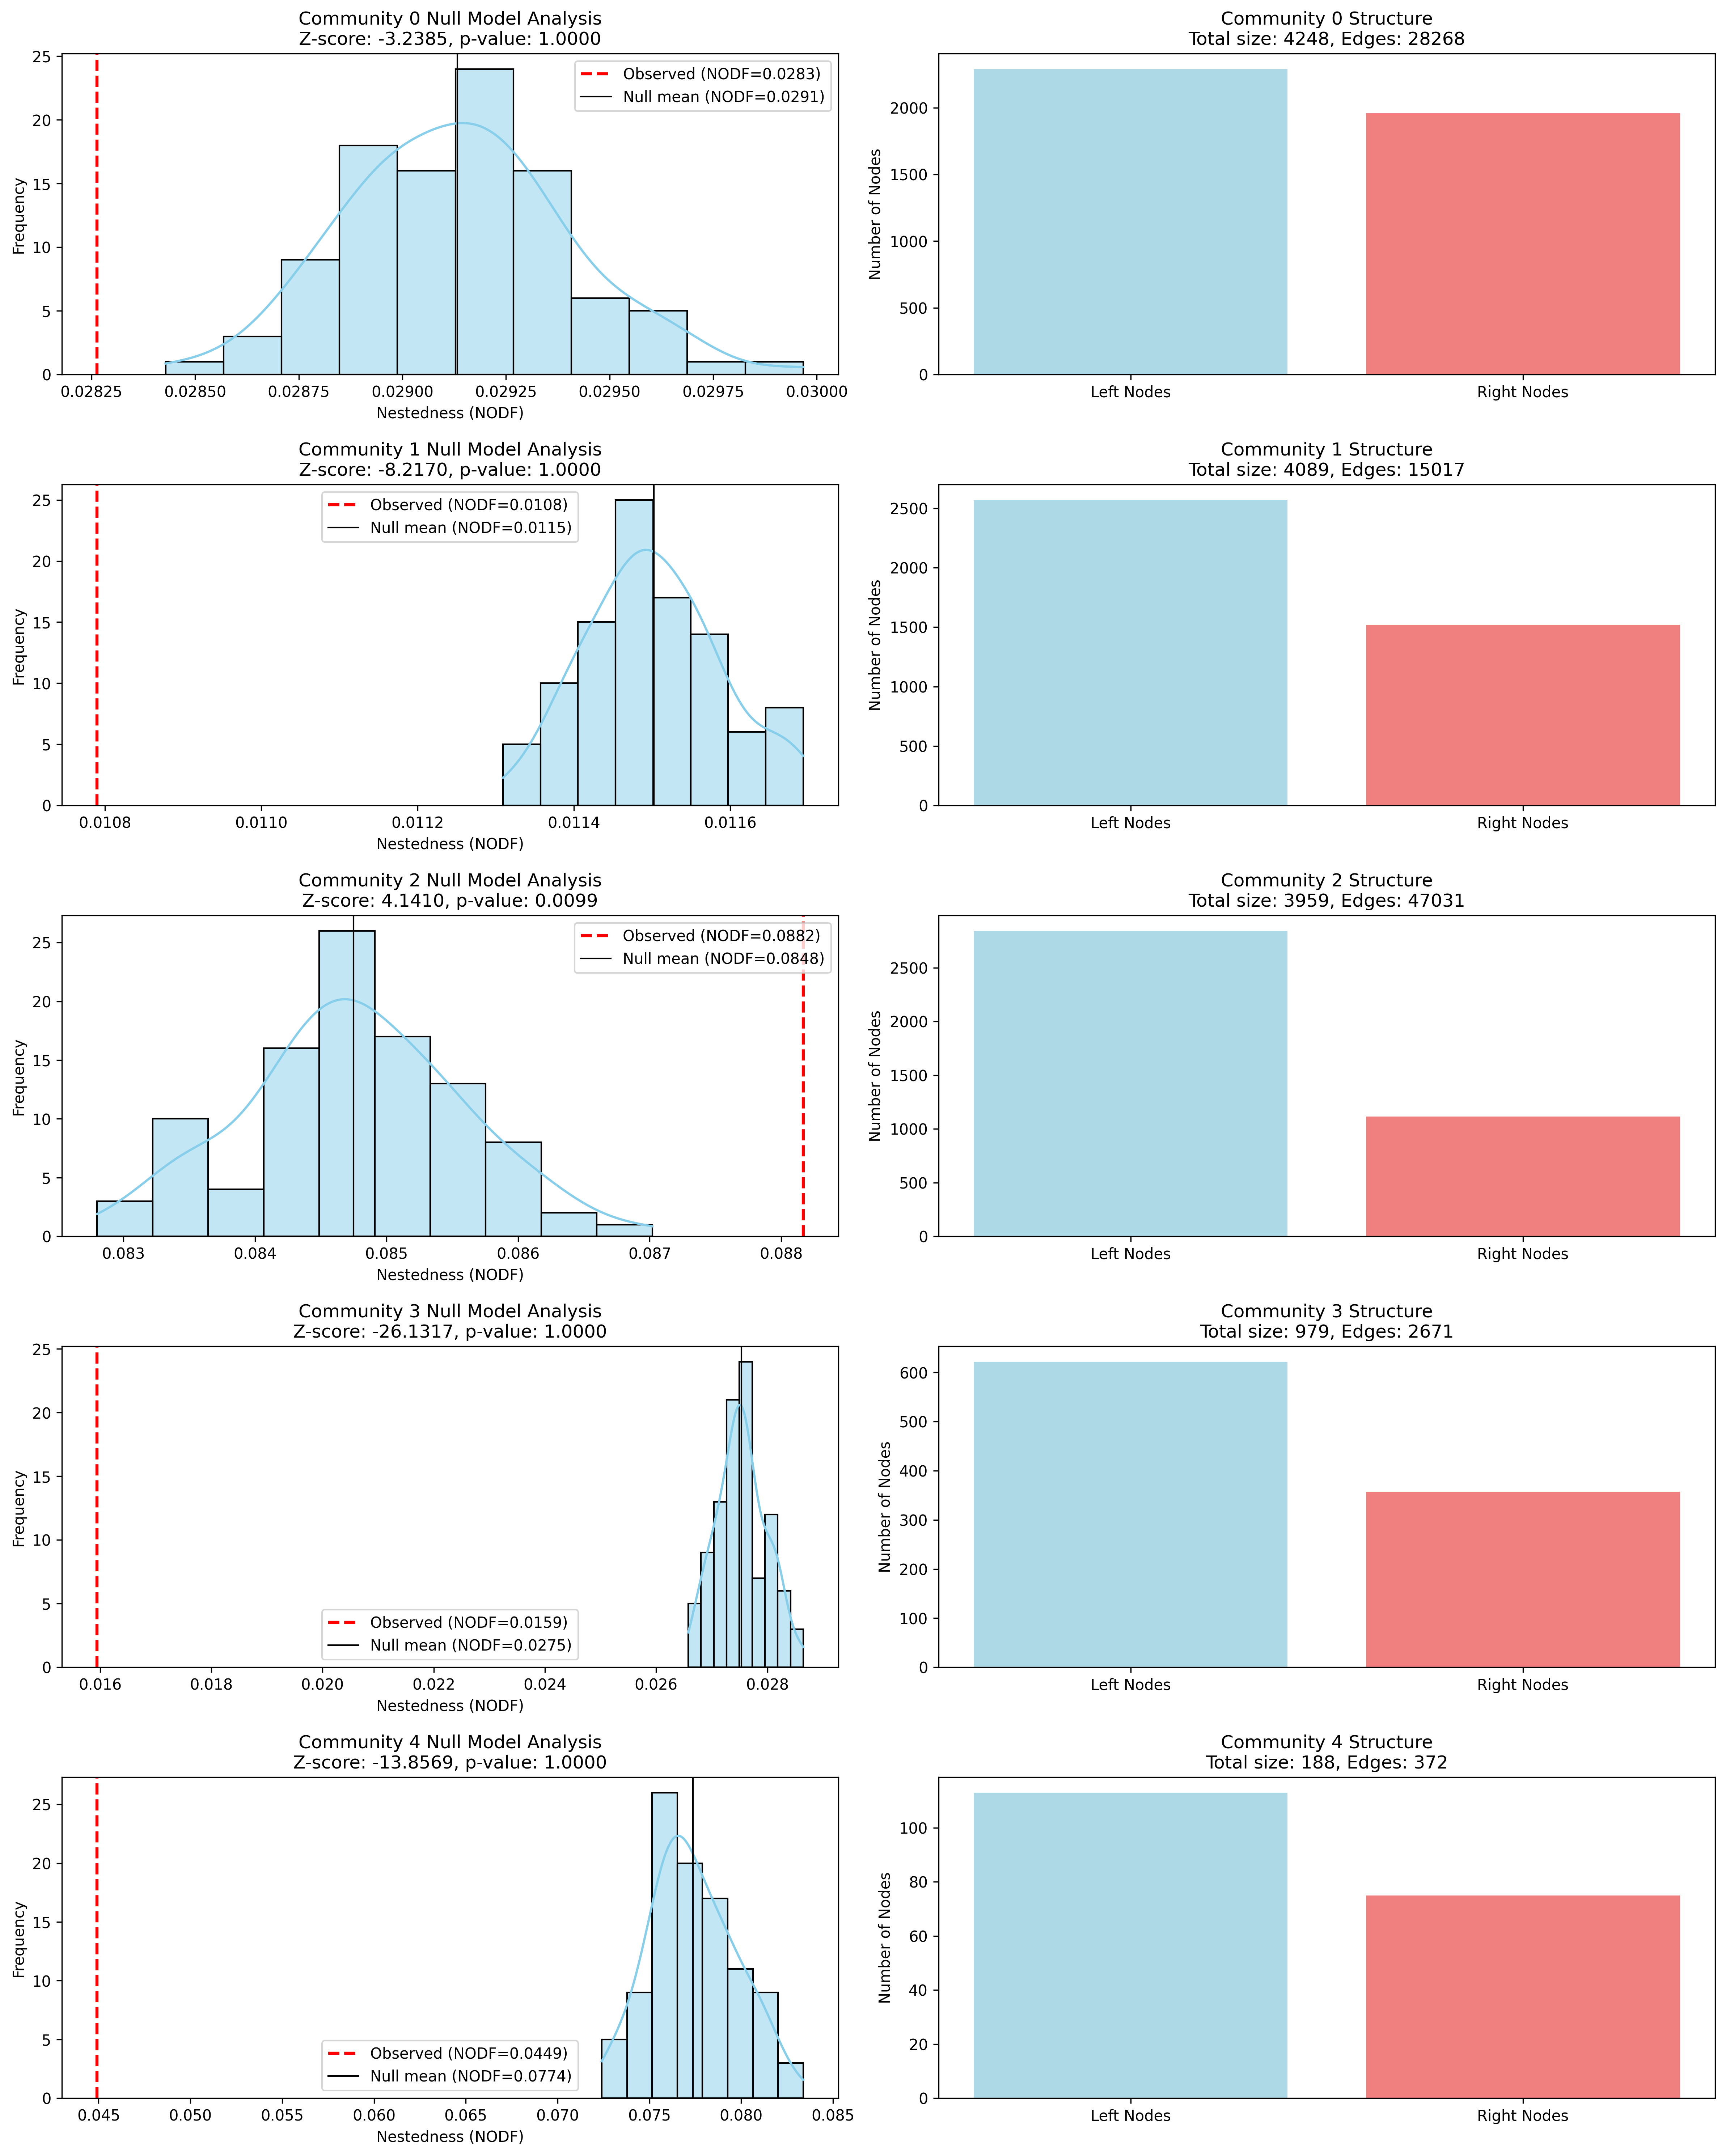
\includegraphics[width=1\textwidth]{../figures/us/significant_communities_detailed.png}
\caption{Comparison of observed versus null model nestedness scores for the five largest investor communities. The diagonal line represents equal observed and expected values, with points above the line indicating higher-than-random nestedness. "Left" refers to late-stage investors, and "Right" refers to early-stage investors.}
\label{fig:nestedness_comparison}
\end{figure}

A broader analysis examining nestedness patterns across all analyzed communities reveals a relationship between community size and nestedness significance, as illustrated in Figure \ref{fig:nestedness_by_community_size}. This analysis examines 8 communities ranging from 122 to 4,248 investors, providing insights into how community structure varies across different organizational scales.

\begin{figure}[htp]
\centering
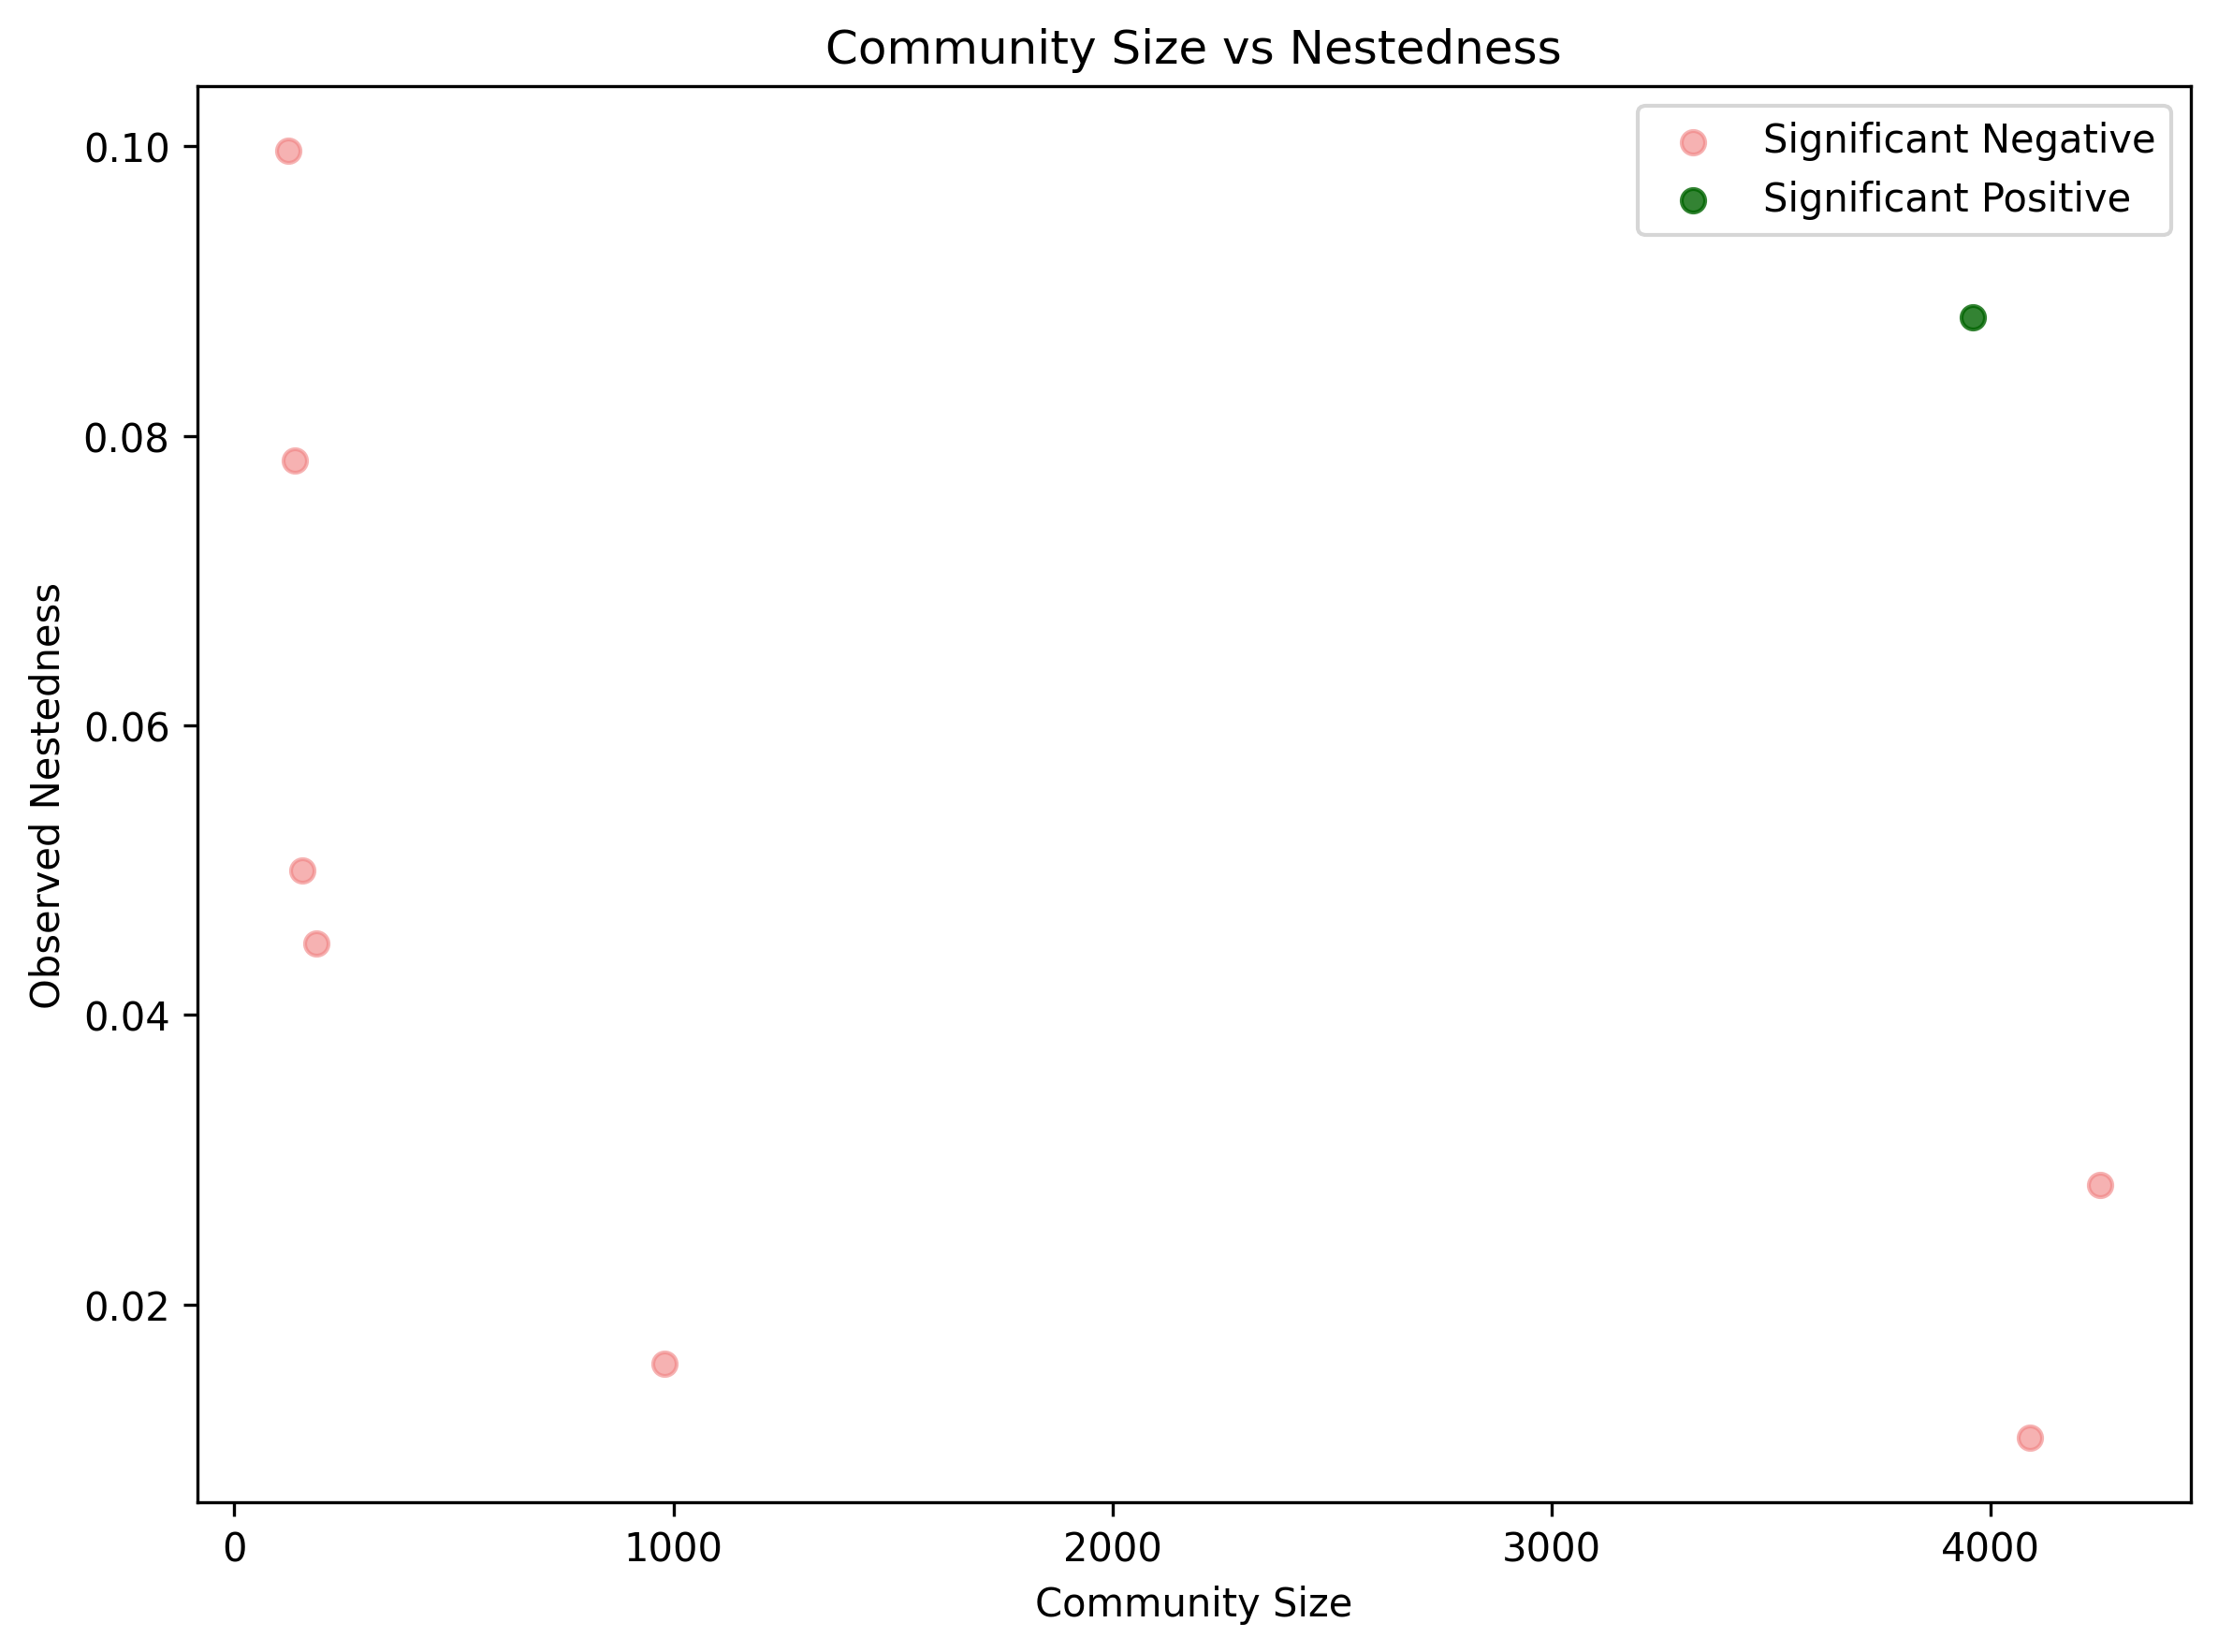
\includegraphics[width=1\textwidth]{../figures/us/nestedness_by_community_size.png}
\caption{Relationship between community size and nestedness significance across all analyzed investor communities. The figure shows observed nestedness scores (y-axis) against community size (x-axis), with markers indicating statistical significance. Only Community 2 exhibits significantly high nestedness, while all other communities show significant low patterns relative to their respective null models.}
\label{fig:nestedness_by_community_size}
\end{figure}

The analysis reveals that high nestedness significance does not follow a simple relationship with community size. While smaller communities (122-188 investors) tend to exhibit higher absolute nestedness scores (0.045-0.099), these values are statistically significant low when compared to appropriate null models. Medium-sized communities (979-4,248 investors) generally show lower absolute nestedness scores (0.011-0.028), with most falling below low nestedness significance thresholds.

Notably, Community 2 stands out as the only community achieving statistically significant nestedness despite having a moderate absolute score (0.088) and being neither the largest nor smallest community analyzed. This pattern suggests that nestedness emergence depends on specific structural characteristics rather than simple community scale effects.

\newcommand{\interestingCommunity}{2}
\newcommand{\interestingCommunityNODF}{0.088}
\newcommand{\interestingCommunityPValue}{0.00001}

Community \interestingCommunity{} demonstrates the most pronounced nestedness, exhibiting an NODF score of \interestingCommunityNODF{} with statistical significance of p = \interestingCommunityPValue{}. This indicates a non-random behavior where less-connected investors maintain co-investment relationships with subsets of partners associated with highly-connected investors, creating a hierarchical investment pattern.

Additionally, Community \interestingCommunity{} exhibits an asymmetric composition with a pronounced ratio favoring late-stage investors over early-stage investors. This imbalance may contribute to the nested structure by creating hierarchical dependencies between investor types.

\todo[inline]{Explore how imbalance contribute to nestedness according to literature}

The following sections provide detailed characterization of the 3 most relevant communities in terms of number of investors, while analyzing in-depth Community 2 (where nestedness was observed) through comparison with Communities 0 and 1, which serve as contrasting examples of similar-sized but differently structured investor networks.

\subsection{Evolution of Nestedness in Silicon Valley Community}

To understand the emergence and development of nested structure, we conducted a temporal analysis of Community 2's nestedness evolution using cumulative window. This analysis reveals how the significantly high nested structure observed in the static analysis developed over time and when it became statistically distinguishable from random network configurations.

The temporal analysis spans 18 years (2007-2024) with sufficient data for nestedness calculation. Early periods (2004-2006) contained insufficient investment activity for meaningful analysis. The evolution demonstrates three distinct phases: an early period with significantly low nestedness (2007-2018), a transition period (2019), and a sustained period with significantly high nestedness (2019-2024).

During the period with significantly low nestedness (2007-2018), observed nestedness scores ranged from 0.15 to 0.38, consistently failing to exceed null model expectations. Z-scores remained predominantly negative, indicating that the observed network structure was less nested than expected under random configuration preserving the degree sequence. This suggests that early venture capital network organization in Community 2 followed patterns that were actually less hierarchical than random syndication among investors with equivalent activity levels.

The transition occurred in 2019, marking the first year when Community 2 achieved significantly high nestedness (Z-score: 2.91, p-value < 0.001). This transition coincided with substantial network growth, reaching 2,364 total nodes and 33,805 edges. 

Notably, the 2019 transition corresponds to the network achieving a connectance threshold of 0.0264, suggesting that nestedness emergence may be related to specific density conditions within large-scale investment networks.

The sustained significant period (2019-2024) demonstrates consistent statistical significance with progressively strengthening Z-scores, reaching a maximum of 4.76 in 2022. 

Interestingly, while absolute nestedness scores decreased from 0.38 in early periods to 0.088 in 2024, the statistical significance increased dramatically. Table \ref{tab:nestedness_evolution_summary} presents key statistics from the temporal evolution analysis.

This apparent paradox reflects the fundamental principle that nestedness significance depends on comparison with appropriate null models rather than absolute magnitude \cite{Mariani2019}.

\begin{table}[htbp]
\hspace*{-1cm}\centering
\begin{tabular}{|c|c|c|c|c|}
\hline
\textbf{Period} & \textbf{Years} & \textbf{Mean NODF} & \textbf{Mean Z-score} & \textbf{Years with High Nestedness} \\
\hline
Low Nestedness (2007-2018) & 12 & 0.2547 ± 0.1158 & -1.4442 ± 1.1108 & 0 \\
Transition (2019) & 1 & 0.1177 & 2.9125 & 1 \\
High Nestedness (2019-2024) & 6 & 0.1012 ± 0.0121 & 3.8950 ± 0.7182 & 6 \\
\hline
\end{tabular}
\caption{Summary statistics for Community 2 nestedness evolution across temporal periods}
\label{tab:nestedness_evolution_summary}
\end{table}

\begin{figure}[htbp]
\hspace*{-1cm}\centering
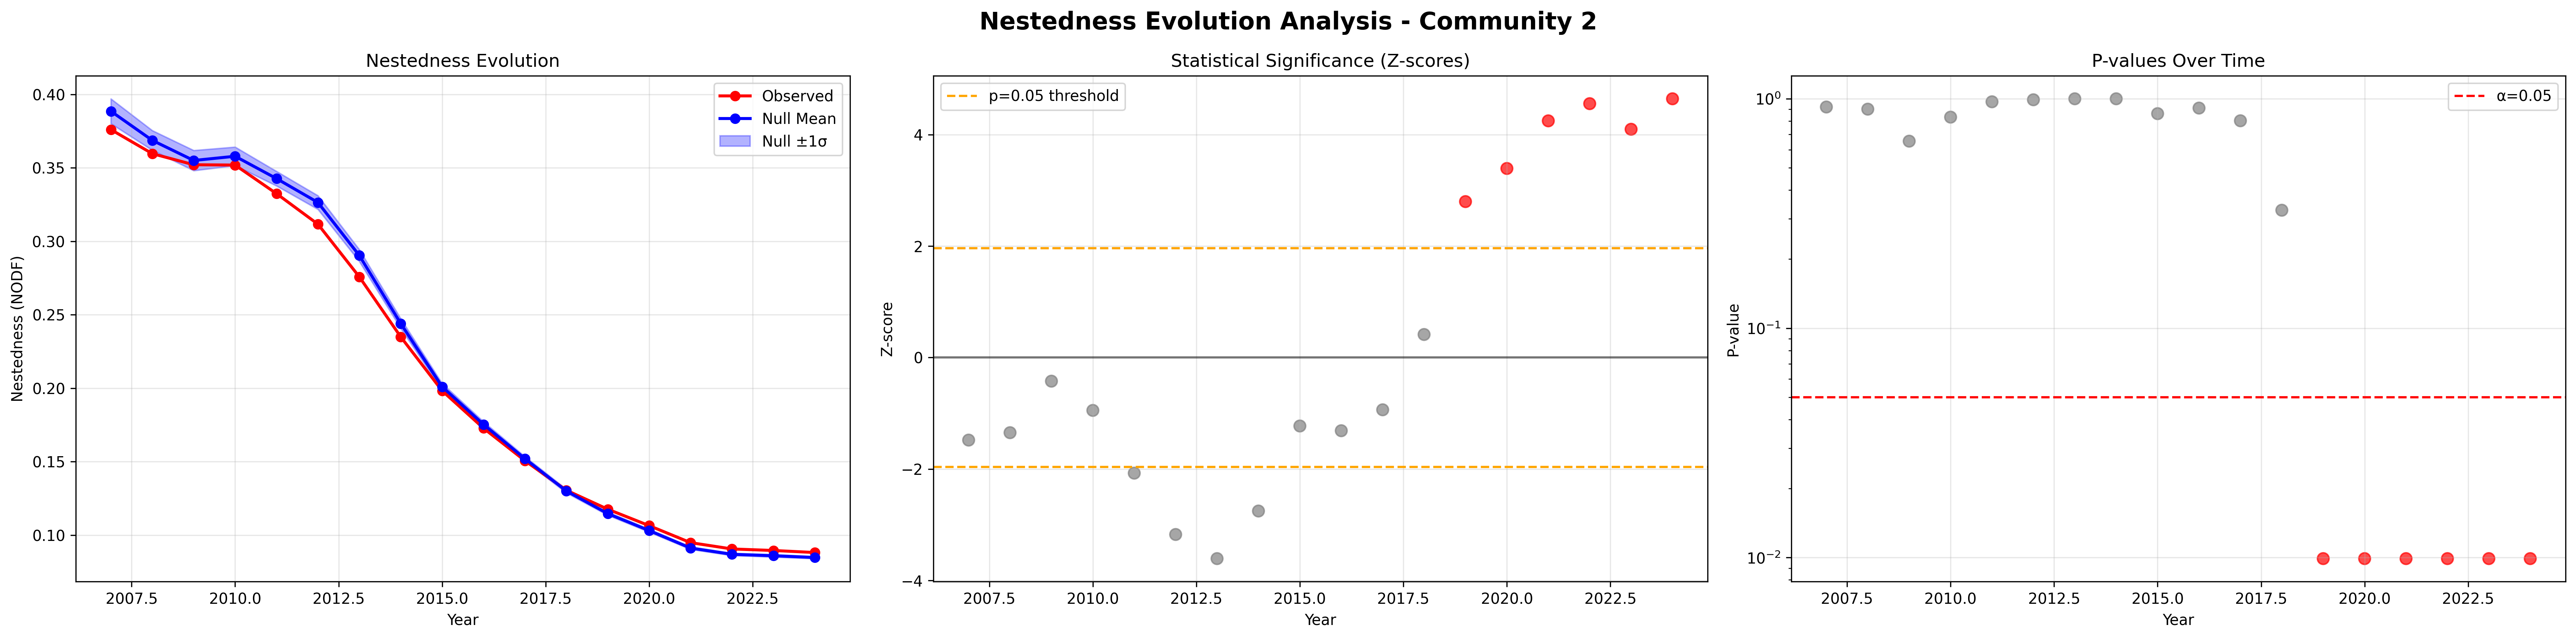
\includegraphics[width=1.2\textwidth]{../figures/us/nestedness_evolution_community_2_pt1.png}
\caption{Temporal evolution of nestedness in Community 2. The left subplot shows the observed nestedness (red) and null model mean (blue) over time, with shaded areas representing the null model standard deviation. The right subplot displays the evolution of network size, with total nodes (green) and total edges (purple) over the same period. The figure highlights the phase transition in 2019, where observed nestedness becomes significantly higher than null model expectations and the network grows rapidly.}
\label{fig:observed_vs_null_model}
\end{figure}

\begin{figure}[htbp]
\hspace*{-1cm}\centering
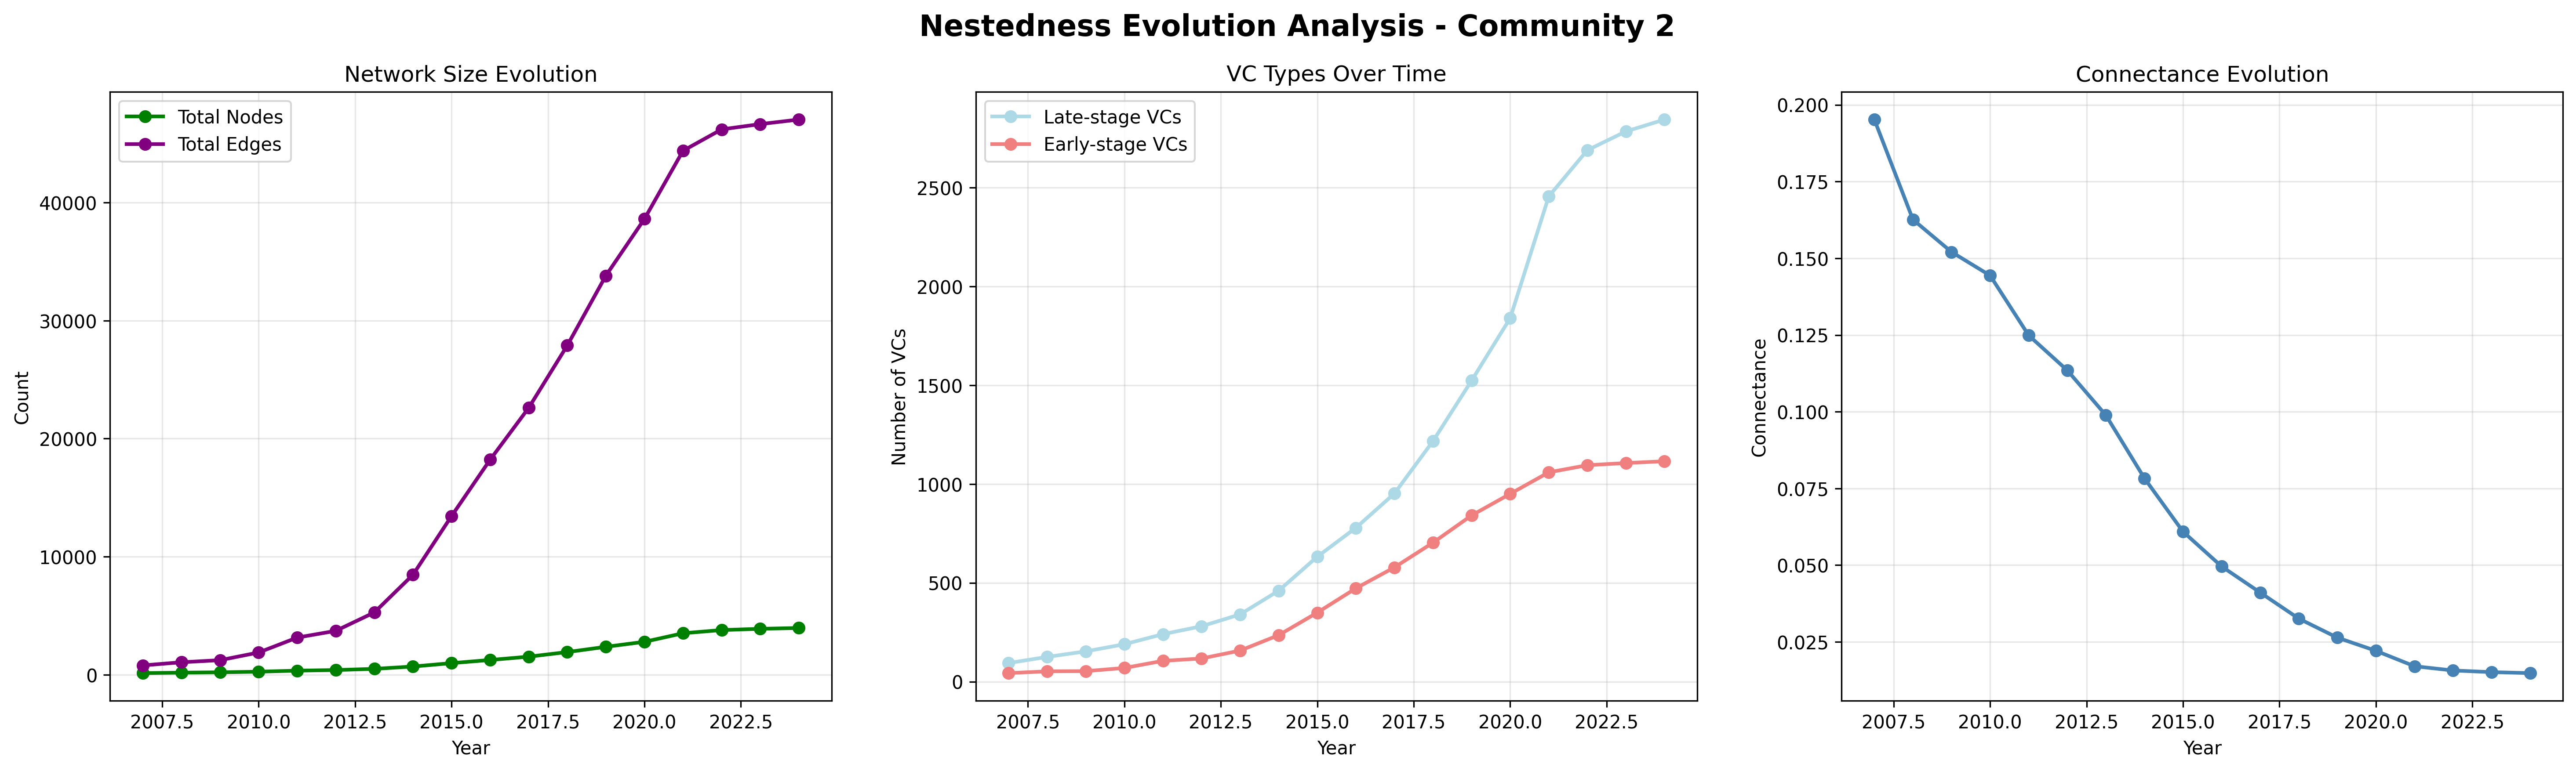
\includegraphics[width=1.2\textwidth]{../figures/us/nestedness_evolution_community_2_pt2.png}
\caption{Connectance and statistical significance evolution in Community 2. The left subplot shows the decreasing trend in connectance (network density) over time, while the right subplot presents the evolution of p-values on a logarithmic scale, indicating the emergence of significantly high nestedness after 2019. The figure demonstrates how the network becomes sparser yet more hierarchically organized, with high nestedness emerging as the network reaches critical size and density thresholds.}
\label{fig:connectance_evolution}
\end{figure}

\begin{figure}[htbp]
\hspace*{-1cm}\centering
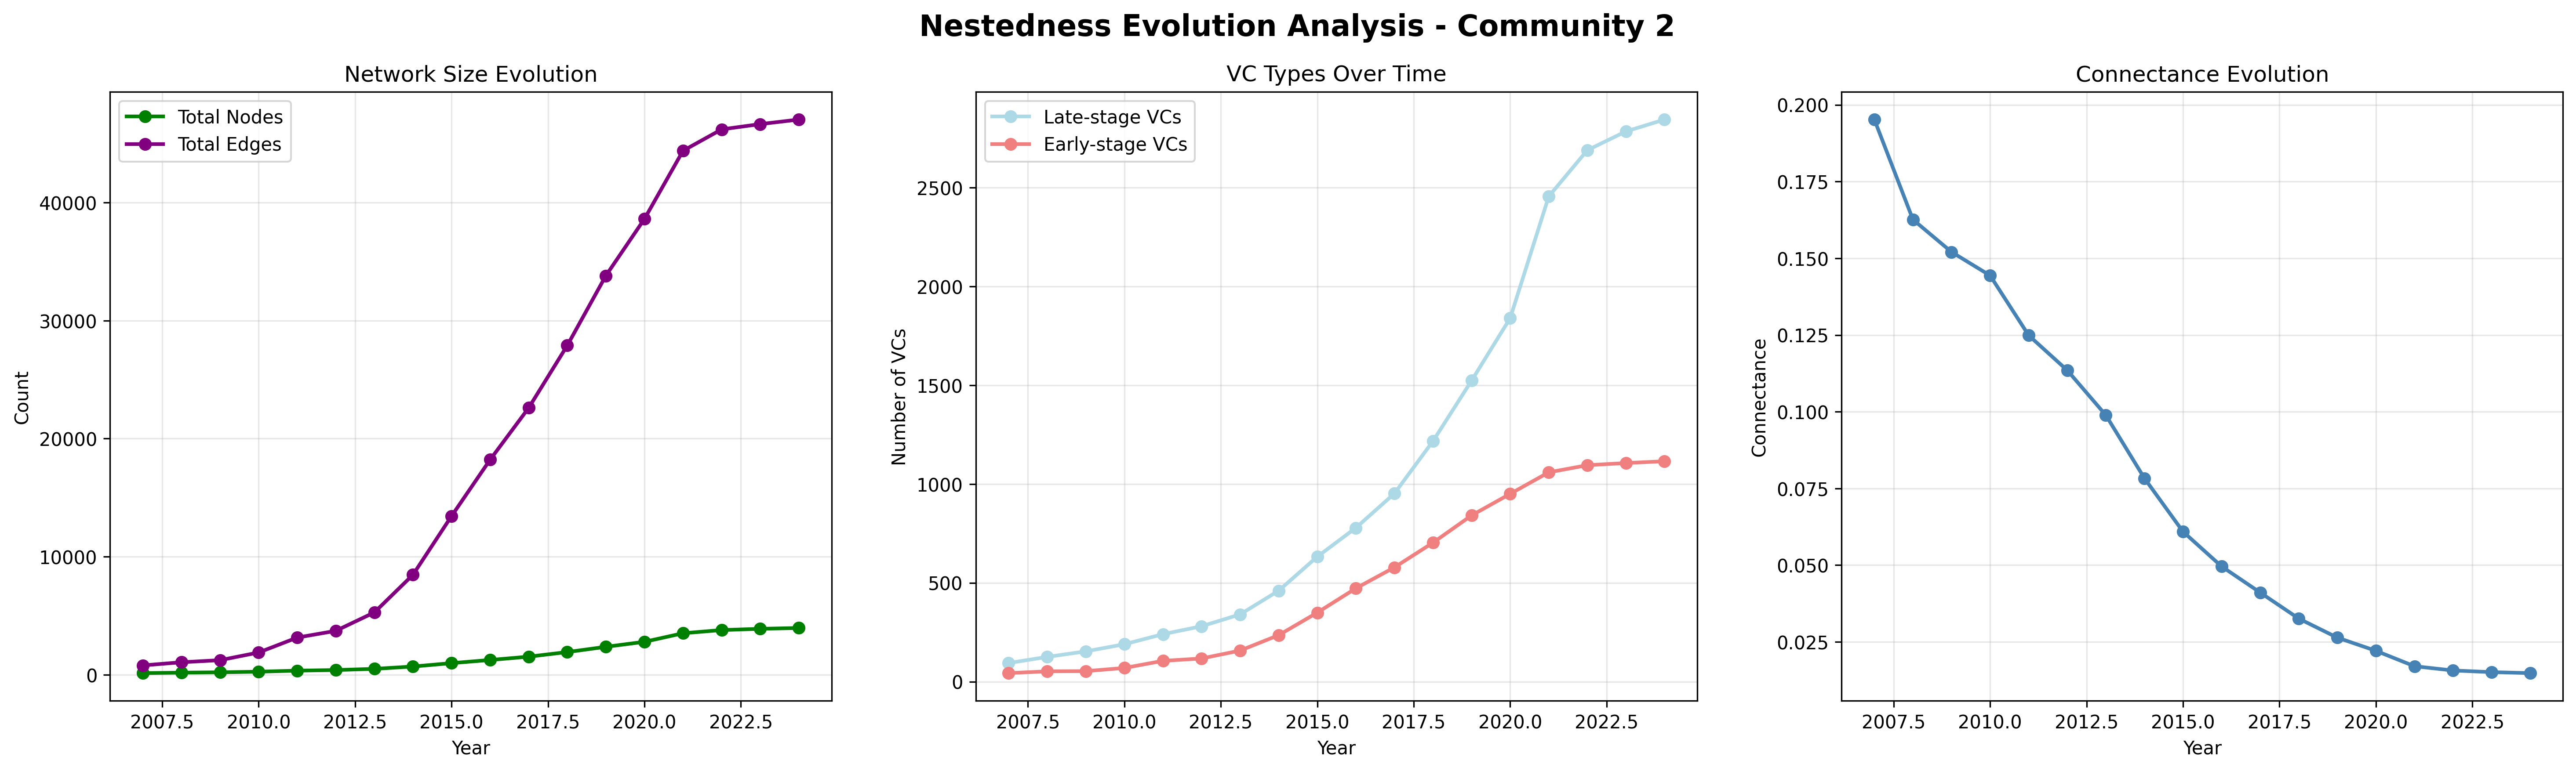
\includegraphics[width=1.2\textwidth]{../figures/us/nestedness_evolution_community_2_pt3.png}
\caption{TBD}
\label{fig:connectance_evolution}
\end{figure}

The analysis reveals several notable patterns in network structure evolution. Late-stage investor participation increased consistently over time, while early-stage investor numbers showed initial growth followed by stabilization after 2020. This asymmetric growth pattern contributed to the development of the nested structure by creating increasingly hierarchical relationships between investor types.

Connectance exhibited a systematic decline from 0.195 in 2007 to 0.015 in 2024, reflecting the network's evolution toward sparser but more strategically organized connections. Despite this decreased density, the emergence of statistical significance suggests that the remaining connections became increasingly hierarchically organized, with less-connected investors maintaining relationships with subsets of the partners of highly-connected investors.

Detailed analysis of the significant periods (2019-2024) reveals consistent patterns in network organization. Each significant year demonstrates similar structural characteristics: large networks (>2,300 nodes), substantial edge counts (>33,000), low connectance (<0.027), and strong statistical significance (Z-scores >2.9). This consistency suggests that the nested structure represents a stable organizational state that persists once established.

\begin{figure}[htbp]
\centering
\includegraphics[width=1\textwidth]{../figures/us/significant_periods_community_2.png}
\caption{Detailed analysis of null model distributions and network structure for key years with significantly high nestedness (2019, 2021, 2024) in Community 2. For each year, the left panel shows the distribution of nestedness scores from degree-preserving null models (blue), with the observed nestedness marked in red. The right panel displays the corresponding network structure, highlighting the number of late-stage and early-stage investors. The figure illustrates the emergence and persistence of significantly high nestedness, as observed values increasingly exceed null model expectations during the high nestedness period.}
\label{fig:null_model_distributions_significant_years}
\end{figure}

The temporal analysis provides evidence that nestedness in venture capital networks emerges through a phase transition process rather than gradual development. The sharp transition from significantly low to significantly high nestedness in 2019, followed by sustained high nestedness, suggests threshold effects in network organization. 

This pattern aligns with theoretical frameworks from complex network theory indicating that certain topological properties emerge discontinuously as networks reach critical size or density parameters \cite{Mariani2019}.

\todo[inline]{Make reflection about possible link with network effects from economics and industrial organization}

The period of nestedness emergence (2019-2024) corresponds with an increase in late-stage investor participation and a relative decrease in early-stage investor numbers within the community. This asymmetric evolution may contribute to the hierarchical structure by creating conditions where early-stage investors increasingly depend on relationships with a subset of the partners associated with highly-connected late-stage investors. 

\todo[inline]{Add reference to figure of nestedness vs null models between 2019 and 2024}

However, whether this temporal correlation reflects causal mechanisms or represents coincidental market dynamics requires further investigation with appropriate theoretical frameworks \cite{Dalle2025}.

\pagebreak